\documentclass[12pt]{report}

% \usepackage{polski}
\usepackage[polish]{babel}
\usepackage[utf8]{inputenc}
\usepackage{mathptmx}
\usepackage{graphicx} % do wstawiania png, pdf
\usepackage{caption} % zmniejszenie rozmiaru podpisów
\usepackage{airtitlepage}
\usepackage{diagbox} % przekątne w komórkach
\usepackage{multirow} 
\usepackage{titlesec} % modyfikacja tytułów
\usepackage{hyperref} % łącza do referencji i w spisach
\usepackage[backend=biber,style=numeric,sorting=none]{biblatex}
\usepackage{rotating} % obracanie
\usepackage{longtable} %tabele na kilku stronach
\usepackage{float}
\usepackage{booktabs} %for \specialrule command
\usepackage{array}
\usepackage{algpseudocode}
\usepackage[shortlabels]{enumitem} % łatwa modyfikacja wyliczenia
\usepackage[titles]{tocloft}
\usepackage[T1]{fontenc} % font times new roman
\usepackage{mathptmx}

%==========Parametry strony tytułowej==========
\uczelniaNazwa{POLITECHNIKA WARSZAWSKA}
\uczelniaLogo{img/pw.pdf}
\wydzial{Wydział Mechatroniki}
\instytut{Instytut Automatyki i Robotyki}
\rok{2017}
\promotor{dr hab. inż. Michał Bartyś}
\temat{Projekt systemu monitorującego zużycie mediów komunalnych}
\autor{Krystian Kałużny}
\miasto{Warszawa}
%==============================================

%====================Wygląd====================
% \setmainfont{Liberation Serif}  %% Najbliższa Times New Roman http://askubuntu.com/questions/346552/closest-alternative-to-times-new-roman
% \setmainfont{Times New Roman}
\linespread{1.3} % odległość między liniami 1.5cm
\setlength{\parindent}{4em} %wielkość wcięcia akapitów

%  Głębokości sekcji
%  \part = -1
%  \chapter = 0
%  \section = 1
%  \subsection = 2
%  \subsubsection = 3
%  \paragraph = 4
%  \subparagraph = 5

\setcounter{secnumdepth}{3} % numeruj do subsubsekcji
\setcounter{tocdepth}{3} % dołącz subsubsekcję do table of content

\titleformat{\chapter}[display]{\normalfont\huge\bfseries}{\chaptertitlename\ \thechapter}{20pt}{\Huge}
\titlespacing*{\chapter}{0pt}{-50pt}{30pt} %{wcięcie poziome}{odstęp od początku strony do "Rozdział X"} {odstęp od tytułu rozdziału do zawartości}
\titleformat{\paragraph}{\normalfont\normalsize\bfseries}{\theparagraph}{1em}{}
\titlespacing*{\paragraph}{0pt}{3.25ex plus 1ex minus .2ex}{1.5ex plus .2ex}

%A4, jednostronny, marginesy
%headsep=1.2cm, headheight=16pt
\usepackage[a4paper, inner=2.5cm, outer=2.0cm, top=2.5cm, bottom=2.5cm]{geometry}
%==============================================
%======================Inne====================
\newcolumntype{C}[1]{>{\centering\let\newline\\\arraybackslash\hspace{0pt}}m{#1}} % definicja typu kolumny: wycentrowanego o określonej szerokości
\newcolumntype{[}[1]{@{\vrule width #1 \hskip\tabcolsep}} % separator kolumn o dowolnej grubości - dla pierwszej kolumny
\newcolumntype{!}[1]{@{\hskip\tabcolsep\vrule width #1 \hskip\tabcolsep}} % separator kolumn o dowolnej grubości - dla środkowych kolumn 
\newcolumntype{]}[1]{@{\hskip\tabcolsep\vrule width #1}}  % separator kolumn o dowolnej grubości - dla ostatniej kolumny
%parametry booktabs
\belowrulesep=0pt
\aboverulesep=0pt

%odstępy w toc
\setlength{\cftbeforechapskip}{.1ex}
\setlength{\cftbeforesecskip}{-.5ex}

% mniejsza czcionka w tabelach
\makeatletter
\renewenvironment{table}{%
	\renewcommand* {\@floatboxreset}{%
		\reset@font\@setminipage}
		\small\@float{table}}
   {\end@float}
\makeatother

% zmniejszenie rozmiaru podpisów
\captionsetup{font=small}
%==============================================

\addbibresource{bibliography.bib}
\begin{document}
	% \nocite{*} %wyświetlenie wszystkich wpisów z bibligrafi (nawet tych nieużywanych)
\pagenumbering{gobble}% Remove page numbers (and reset to 1)

% \thispagestyle{empty}

\vspace*{2cm}

\begin{center}
	\textbf{Życiorys}
\end{center}
\begin{figure}[ht] %pływające otoczenie, h - zacznij tam gdzie zaczyna się tekst, t - umieść na górze strony
	\begin{minipage}[b]{0.35\textwidth} %minipage - niezależny alias strony
		\centering
		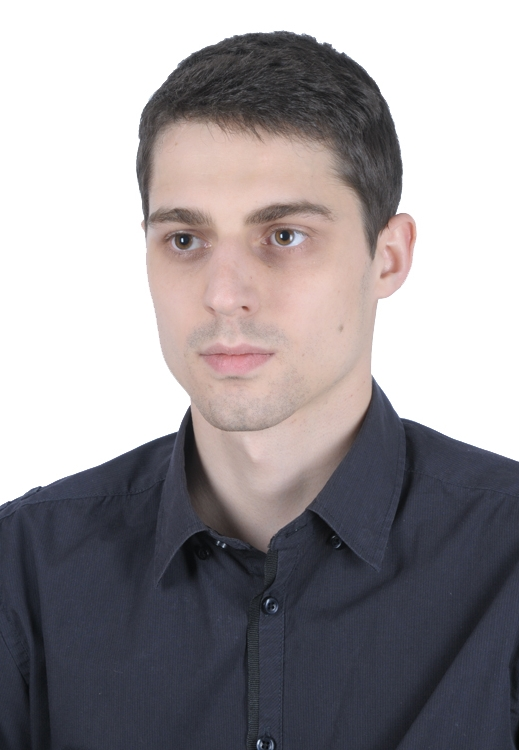
\includegraphics[width=\textwidth]{img/me-cv.jpg}
	\end{minipage}
	\hspace{0.5cm}
	\begin{minipage}[b]{0.6\textwidth}
		\begin{flushleft}
		Ireneusz Szulc
		
		{\it Kierunek:} Automatyka i Robotyka
		
		{\it Specjalność: } Informatyka przemysłowa
		
		{\it Urodzony:} 21. marca 1993~r. w Lublinie.
		
		{\it Numer indeksu:} 251001
		
		\end{flushleft}
	\end{minipage}
\end{figure}

Urodziłem się w Bździszewie.
W 2009 roku ukończyłem Gimnazjum w Woli Uhruskiej.
Następnie uczęszczałem do I Liceum Ogólnokształcącego im. Stefana Czarnieckiego w Chełmie.
W 2012 zdawałem maturę na poziomie rozszerzonym z matematyki i fizyki. 
Po maturze kontynuowałem naukę na Politechnice Warszawskiej na Wydziale Mechatroniki na kierunku Automatyka i Robotyka. 

\vspace{2cm}

\begin{flushright}
%bez wcięcia
	\noindent...................................
\end{flushright}

\stronatytulowa %własna strona tytułowa

% \newgeometry{tmargin=0cm, bmargin=0cm, lmargin=0cm, rmargin=0cm}
\begin{figure}[t]
	\centering
	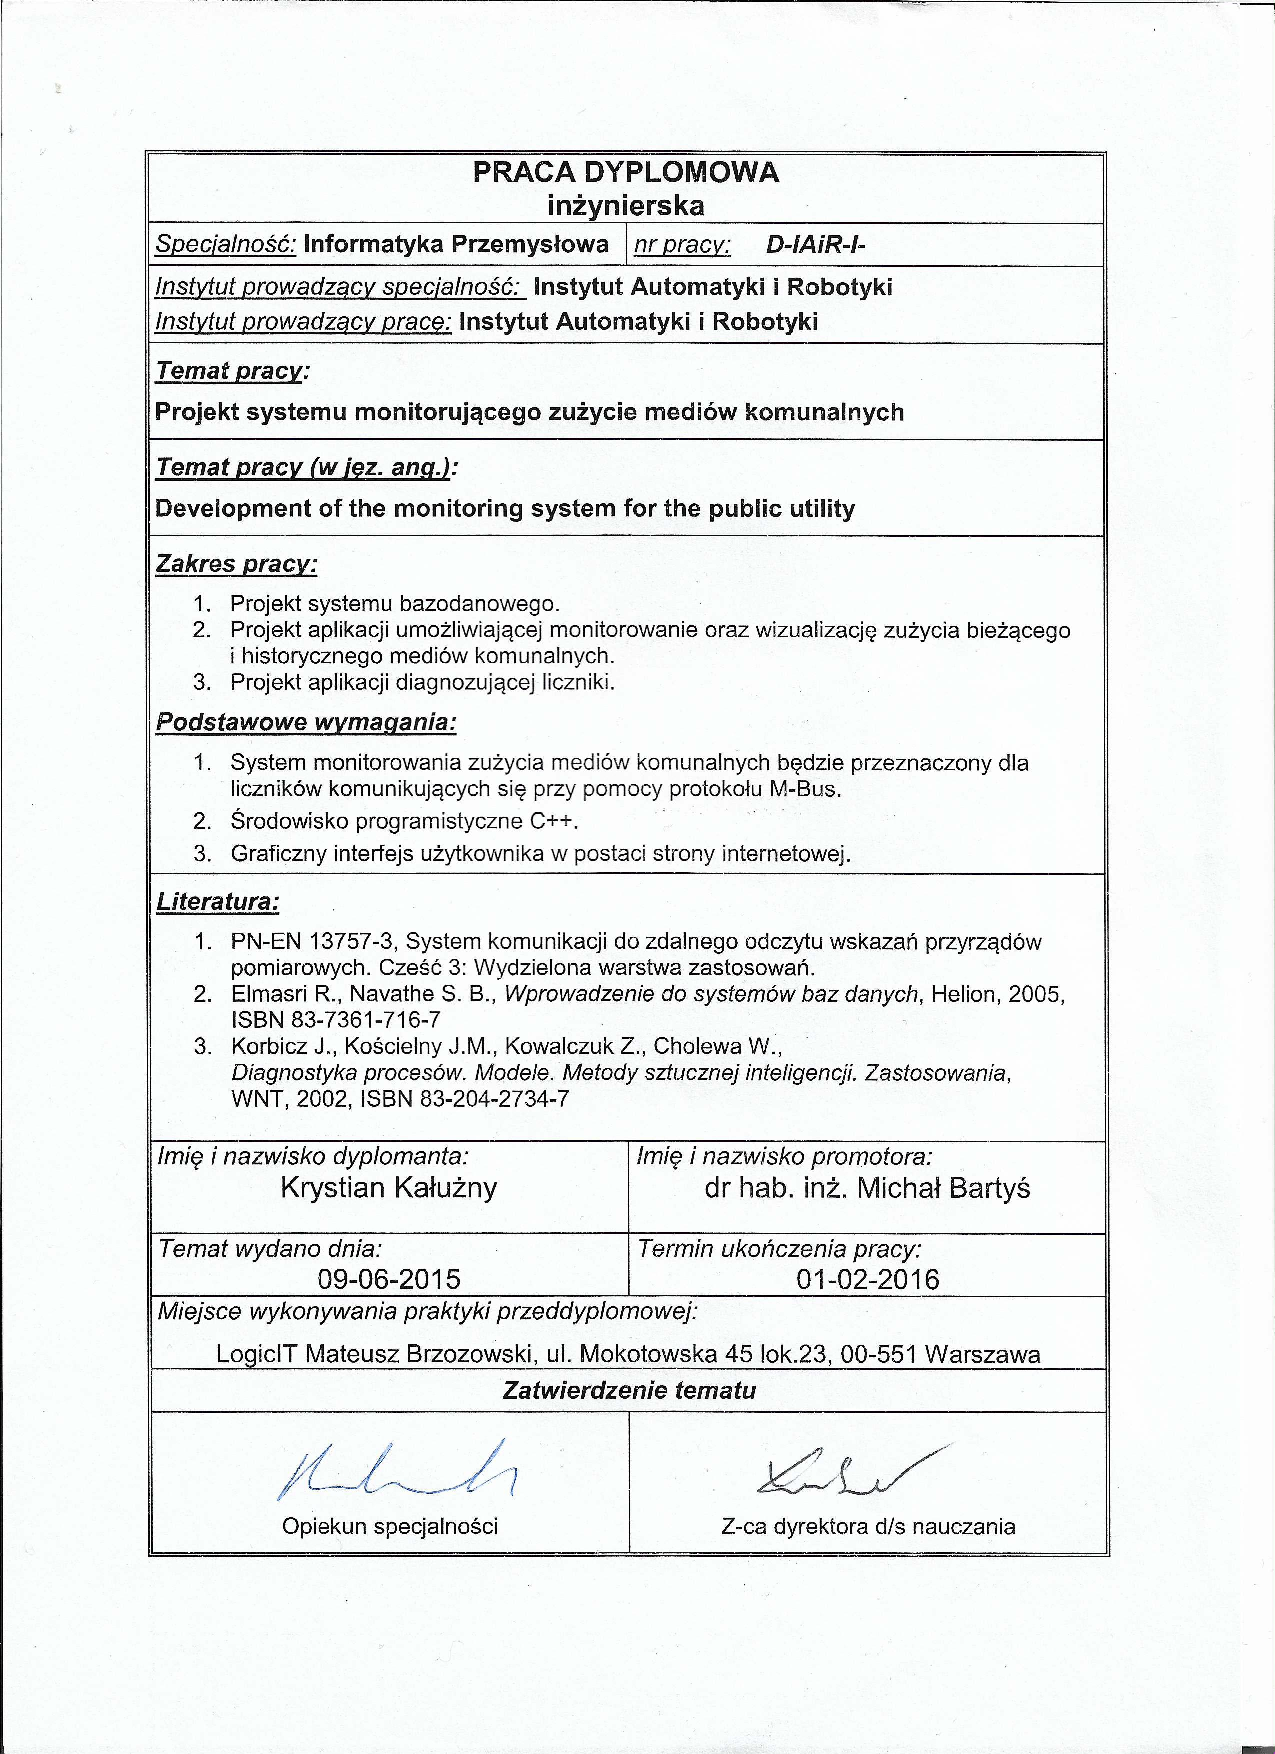
\includegraphics[scale=1.0]{img/karta-tematu.pdf}
	\label{fig:karta_tematu}
\end{figure}
\restoregeometry

% \noindent {\Large\textbf{Streszczenie}}

Niniejsza praca na celu zaprojektowanie oraz stworzenie systemu do monitorowania zużycia mediów komunalnych.
System ma współpracować z licznikami mediów wyposażonymi w interfejs komunikacyjny M-Bus.
System ma przedstawiać aktualne stany liczników oraz wizualizować historyczne zużycie mediów.
Dodatkowym zadaniem systemu jest tworzenie i analiza profili zużycia mediów komunalnych.
Analiza profilu ma na celu określenie czy aktualna wartość zużycia odbiega, w sposób znaczący, od wartości przewidywanej.
System ma informować o zaistniałych odejściach od wartości oczekiwanej oraz innych błędach, które mogą świadczyć o uszkodzeniu liczników lub infrastruktury doprowadzającej media.
Praca skupia się na współpracy systemu z licznikami wody.

Do zadań projektu należało stworzenie oprogramowania zajmującego się odczytem liczników zgodnie z protokołem M-Bus oraz interfejsu użytkownika udostępniającego, w przystępny sposób, zebrane dane.

W pierwszej części pracy został opisany protokół M-Bus z podziałem na warstwę fizyczną, łącza danych, aplikacji oraz zarządzania.
Przedstawione zostały tryby transmisji danych, formaty ramek telekomunikacyjnych, struktury rekordów z danymi oraz sposób zwiększenia obsługiwanej liczby urządzeń w sieci, dzięki rozszerzonemu adresowaniu.
Opis jest zgodny z normą PN-EN 13757-3:2013.

Ponieważ działanie systemu miało zostać przetestowane na licznikach wody, kolejna część pracy zawiera opis najczęściej używanych wodomierzy.
Są to wodomierze wirnikowe oraz komorowe służące często do wzorcowania tych pierwszych.
Przedstawione zostały ich schematy oraz zasady działania.

Dalej znajduje się opis dostępnego rozwiązania o podobnym zastosowaniu ZENNER Bus-System.
Zaprezentowane zostały urządzenia komunikacyjne współpracujące z magistralą M-Bus.

Kolejna część pracy przedstawia zbiór wymagań dotyczących działania systemu oraz sposób ich implementacji w wyniku, której powstały dwa podprojekty odpowiedzialne odpowiednio za odczytywanie danych z liczników oraz wyświetlanie tych danych na stronie WWW.
Wyznaczona zostaje tu wartości interwału odczytów.
Następnie zostaje zaprezentowany główny algorytm  programu odczytującego wraz z opisem klas występujących projekcie.

Ostatnia część zawiera opis testów systemu, mających na celu sprawdzenie zgodności z postawionymi wcześniej wymaganiami.
Testy zostały zrealizowane przy pomocy dostępnych wodomierzy oraz specjalnie do tego stworzonej aplikacji symulującej licznik.

\pagebreak

\noindent {\Large\textbf{Abstract}}


\pagebreak

\tableofcontents

\pagebreak
\pagenumbering{arabic}% Arabic page numbers (and reset to 1)

% \chapter{Wprowadzenie} % (fold)
\label{cha:wprowadzenie}

Celem pracy jest zaprojektowanie i stworzenie systemu do monitorowania zużycia mediów komunalnych takich jak woda czy gaz.
System ten ma być przeznaczony do współpracy z licznikami mediów wyposażonymi w interfejs komunikacyjny M-Bus.
Poza przedstawieniem aktualnych stanów liczników, system powinien pozwalać na wizualizację historycznego zużycia mediów.

Projektowany system ma być przeznaczony do użytku w budynkach mieszkalnych.
Nie można zatem zakładać, że użytkownikami systemu będą osoby znające zagadnienia techniczne związane z protokołem komunikacyjnym M-Bus.
Należy więc stworzyć prosty i intuicyjny interfejs graficzny, na którym będą prezentowane tylko niezbędne informacje.

Dane o zużyciu powinny być dostępne poprzez sieci LAN oraz WiFi, jako że obecnie są one bardzo popularne i używane w wielu domach.
Najprostszym sposobem na osiągnięcie tego celu jest udostępnianie ich za pomocą strony WWW.
Umożliwi to dostęp do danych zarówno z komputerów typu PC, laptopów jaki i tabletów czy smartfonów.

System powinien również wykrywać błędy, mogące pojawić się w trakcie użytkowania, takie jak brak połączenia z podsystemami i urządzeniami składowymi, odłączenia lub uszkodzenia liczników.
Informacje o wykrytych błędach powinny być dostępne z poziomu interfejsu graficznego w postaci strony WWW.

Dodatkową funkcjonalnością jaką powinien zapewniać system jest analiza profilów zużycia mediów dla poszczególnych liczników należących do systemu.
Aby stworzyć profile zużycia wymagane jest możliwie częste odczytywanie liczników i przechowywanie wszystkich historycznych danych.
Profile powinny być ciągle uaktualniane, aby odzwierciedlić jak najlepiej charakter zmian zużycia mediów.
Dzięki wyznaczonemu profilowi możliwe będzie sprawdzenie, czy aktualne zużycie danego medium znaczącą odbiega od przewidywanej wartości lub czy nie.
Przypadki wyraźnej niezgodności z profilami zużycia mediów mogą oznaczać uszkodzenia infrastruktury doprowadzającej lub uszkodzenia liczników i powinny być raportowane podobnie jak błędy.

Projektowany system może być stosowany do celów rozliczeniowych oraz kontrolnych, np. w mieszkaniach wynajmowanych, gdzie właściciel nie mam możliwości bezpośredniego sprawdzenia stanów liczników.

Praca skupia się na badaniu współpracy systemu z licznikami wody.
Jednak system powinien działać poprawnie z 250 licznikami dowolnych mediów komunalnych, niezależnie od ich modelu czy producenta.
% chapter wprowadzenie (end)

	
% \chapter{Implementacja}
\label{cha:implementacja}

\section{Wymagania}

W stosunku do urządzenia typu master w sieci M-Bus, postawiono następujące wymagania funkcjonalne:
\begin{itemize}
	% \itemsep 0em 
	\item przedstawianie ostatnich znanych stanów liczydeł wodomierzy,
	\item możliwie częste odczytywanie stanu wodomierzy,
	\item obsługa do 250 urządzeń typu slave w sieci,
	\item automatyczne wykrywanie nowych urządzeń dołączonych do sieci,
	\item wizualizację zużycia wody z wybranego okresu,
	\item wykrywanie i notyfikacja odłączenia wodomierza od sieci,
	\item wykrywanie i notyfikacja przekroczeń zużycia wody.
	% \item wykrywanie i notyfikacja braków zużycia wody.
\end{itemize}

Program komunikujący się z urządzeniami typu slave w sieci M-Bus miał zostać zaimplementowany w języku programowania C++.
Natomiast wszelkie wizualizacje danych oraz notyfikacje problemów miały być zrealizowane za pomocą strony internetowej.

\section{Stanowisko badawcze}

Stanowisko badawcze składa się mikrokomputera Odroid C1+, konwertera Ethernet/M-Bus ETH2,
wodomierza z modułem komunikacyjnym M-Bus, wodomierza z modułem komunikacji impulsowej oraz modułu zliczającego impulsy firmy ZENNER.
Schemat połączenia elementów na stanowisku badawczym przedstawia rysunek \ref{fig:diagram_of_test_bench}.

\begin{figure}[ht]
	\centering
	\includegraphics[height=6cm]{img/schemat_stanowiska.png}
	\caption[Schemat stanowiska badawczego]{Schemat stanowiska badawczego [źródło własne]}
	\label{fig:diagram_of_test_bench}
\end{figure}

Odroid C1+ wyposażony jest w czterordzeniowy procesor o maksymalnej częstotliwości taktowania $ 1.5\ GHz $ zbudowanego w architekturze ARMv7,
$ 1GB $ pamięci RAM DDR3, gniazdo Ethernet, 4 wyjścia USB 2.0 oraz kartę microSD o pojemności $ 32GB $ \cite{odroid_c1_plus}.
Na karcie microSD został zainstalowany system Ubuntu 16.04.

\begin{figure}[ht]
	\centering
	\includegraphics[height=5.5cm]{img/ODROID_C1_BoardDetail.jpg}
	\caption[Odroid C1+ schemat]{Odroid C1+ schemat \protect\cite{odroid_c1_plus}}
	\label{fig:odroid_c1_plus}
\end{figure}

Konwerter ETH2 służy do konwersji standardu ethernetowego 10Base-T na M-Bus master oraz na RS232.
Umożliwia podłączenia 10 urządzeń typu M-Bus slave.
Eth2 obsługuje protokoły sieciowe TCP/IP, UDP, ICMP, DHCP oraz ARP.
Urządzenie wykorzystuje moduł EM100 firmy Tibbo Technology do komunikacji oraz konfiguracji \cite{eht2}.
Konwerter można konfigurować poprzez łącze RS232, ethernet UDP lub ethernet TCP.
Konfiguracja odbywa się za pomocą dedykowanego oprogramowania Device Server Toolkit dla modułu EM100 lub komend przesyłanych przez ethernet lub port szeregowy \cite{tibbo_commands}.
Eth2 posiada również trzy wejścia stykowe beznapięciowe oraz jedno wyjście dwustanowe.

Wodomierze wchodzące w skład stanowiska to wodomierze jednostrumieniowe firmy Itron (rysunek \ref{fig:single_jet_watermeter}).
Jeden z nich jest wyposażony w moduł M-Bus \cite{itron_produkty} i jest bezpośrednio podłączany do magistrali.
Drugi natomiast posiada moduł impulsowy \cite{itron_produkty}, który jest podłączony do modułu zliczającego impulsy firmy ZENNER.
Stała impulsowania tego modułu wynosi $ 10\ dm^3 / imp $.


\begin{figure}[ht]
	\centering
	\begin{minipage}{0.47\textwidth}
 		\centering
		\includegraphics[height=6cm]{img/ETH2.jpg}
		\caption[Konwerter Eth2]{Konwerter Eth2 \protect\cite{eht2_online}}
		\label{fig:odroid_c1_plus}
	\end{minipage}%
	~
	~
	~
	\begin{minipage}{0.47\textwidth}
 		\centering
		\includegraphics[height=6cm]{img/jednostrumieniowy_itron.jpg}
		\caption[Wodomierz jednostrumieniowy Itron]{Wodomierz jednostrumieniowy Itron [źródło własne]}
		\label{fig:single_jet_watermeter}
	\end{minipage}%
\end{figure}

Moduł zliczający impulsy posiada trzy wejścia impulsowe oraz interfejs M-Bus, obsługujący prędkość transmisji $ 2400\ b/s $.
Moduł zasilany jest bateryjnie.
Maksymalny czas pracy wynosi 6 lat.

\section{Projekt aplikacji UMonit}

W celu realizacji zdefiniowanych wymagań projektowych zrealizowano projekt o nazwie UMonit (UtilityMonit).
Ze względu na specyfikację, projekt UMonit został podzielony na dwa podprojekty UMonitApp oraz UMonitWeb.

\subsection{UMonitApp}

UMonitApp jest programem odczytującym stany liczników za pomocą interfejsu Ethernet konwertera ETH2.
Zadaniem programu ma być odczytywanie do 250 urządzeń w jak najkrótszym czasie, wykrywanie odłączeń i dołączeń urządzeń,
wykrywanie znaczących różnic w stosunku do przewidywanego dobowego zużycia wody oraz udostępnianie zebranych danych aplikacji UMonitWeb.

\paragraph{Wyznaczenie interwału odczytów wodomierzy}

Aby dobrać odpowiedni interwał odczytu wodomierzy należy oszacować przewidywany czas obsługi urządzeń zgodnie z normą \cite{pnen137573}.
Rozważmy dwa przypadki konfiguracji sieci, kiedy nie ma podłączonych urządzeń do magistrali oraz przypadek kiedy jest do niej dołączonych 250 urządzeń.
Do wyliczeń będą potrzebne wartości czasu transmisji jednego bitu oraz bajtu.

Czas transmisji jednego bitu wynosi:
\begin{equation}
	\label{eq:bit_time}
	T_b = \frac{1}{2400} = 0,000417 s
\end{equation}

Czas transmisji jednego bajtu uwzględniając bit startu, parzystości i stopu wynosi:
\begin{equation}
	\label{eq:byte_time}
	T_B = T_b \cdot 11 = 0,004583 s
\end{equation}

Przy braku odpowiedzi urządzenia o zadanym adresie master po czasie równym czasowi transmisji $ 330 $ bitów plus $ 50\ ms $ ponawia żądanie.
Master może wysłać dane żądanie trzykrotnie zanim przejdzie do komunikacji z kolejnym urządzeniem.
Przed wysłaniem kolejnego żądania należy wprowadzić czas bezczynności równy czasowi transmisji $ 33 $ bitów.
Dla braku wszystkich 250 urządzeń otrzymujemy:
\begin{equation}
	\label{eq:no_devices_time}
	T_1 = \big((330 \cdot T_b + 0,05) \cdot 3 + 33 \cdot T_b \big) \cdot 250 = 0,576591 \cdot 250 = 144,147750 s
\end{equation}

Kiedy 250 urządzeń typu slave jest podłączonych do magistrali oraz każde odpowiada ramką danych o maksymalnej długości $ 261 $ to czas odpowiedzi wszystkich urządzeń wynosi:
\begin{equation}
	\label{eq:all_devices_time}
	T_2 = (T_B \cdot 261) \cdot 250 = 1,196163 \cdot 250 = 299,040750 s
\end{equation}

Aby oszacować całkowity czas komunikacji pomiędzy jednostkami master i slave, należy do $ T_1 $ oraz $ T_2 $ dodać czas transmisji żądań mastera.
Master wysyła żądania REQ\_UD2 w postacie krótkiej ramki, która składa się z 5 bajtów.
\begin{equation}
	\label{eq:req_time}
	T_{req} = (T_B \cdot 5) \cdot 250 = 0,022915 \cdot 250 = 5,728750 s
\end{equation}

Zatem całkowity czas obsługi magistrali bez urządzeń oraz magistrali z 250-oma urządzeniami wynosi odpowiednio $ T_{c1} $ i $ T_{c2} $:
\begin{equation}
	\label{eq:no_device_total_time}
	T_{c1} = T_1 + T_{req} = 149,8765 s \approx 2,5 min
\end{equation}
\begin{equation}
	\label{eq:all_device_total_time}
	T_{c2} = T_2 + T_{req} = 304,7695 s \approx 5,1 min
\end{equation}

Należy pamiętać o możliwości występowania innych opóźnień, takich jak na przykład oczekiwanie na połączenia TCP z urządzeniem ETH2.
Można zatem, z pewnym nadmiarem, przyjąć wartość interwału odczytów równą $ 6\ min $.

\paragraph{Schemat aplikacji UMonitApp}

Podprojekt UMonitApp został napisany z użyciem biblioteki Qt w wersji 5.5.
Qt jest międzyplatformowym narzędziem do tworzenia aplikacji okienkowych, konsolowych i wbudowanych \cite{qt}.
Biblioteka ta pozwala na prostą i bezpieczną komunikację między różnymi komponentami aplikacji,
które w szczególności mogą znajdować się w różnych wątkach, za pomocą mechanizmu sygnałów i slotów.
Qt udostępnia między innymi moduł do obsługi baz danych SQL oraz moduł do komunikacji sieciowej.
Aplikacja używa bazy SQLite.
UMonitApp korzysta również z biblioteki inteligentnych wskaźników zawartych w zbiorze bibliotek C++ boost.
Inteligentne wskaźniki pozwalają na automatyczne zwalnianie zaalokowanej pamięci, kiedy ta przestanie być już używana \cite{smart_ptr}.

Do udostępniania danych o licznikach, zużyciu oraz alarmach dla aplikacji UMonitWeb wykorzystano bibliotekę \textit{QttpServer}.
Biblioteka ta pozwala w prosty sposób stworzyć serwer z HTTP API, a w szczególności RESTful serwer.
QttpServer wykorzystuje  bibliotekę \textit{node.native} do uruchomienia serwera http.
Z kolei node.native bazuje na \textit{libuv}; bibliotece, która służy do obsługi asynchronicznych zadań wejściowo - wyjściowych, między innymi zajmuje się asynchronicznymi socketami TCP, UDP i dostępem do systemu plików.
Zdarzenia generowane przez libuv przenoszone są do pętli zdarzeń qt aplikacji zawierającej QttpServer (rysunek \ref{fig:qttpserver_eventloop}).
Jej zaletą jest łatwa integracja z aplikacjami pisanymi z użyciem biblioteki Qt \cite{qttpserver}.

\begin{figure}[ht]
	\centering
	\includegraphics[height=7cm]{img/qttp_eventloops.png}
	\caption[Schemat przepływu zdarzeń w QttpServer]{Schemat przepływu zdarzeń w QttpServer \protect\cite{qttpserver}}
	\label{fig:qttpserver_eventloop}
\end{figure}

Aplikacja UMonitApp została podzielona na dwie części, które uruchomione są w dwóch różnych wątkach.
Pierwsza cześć zajmuje się dokonywaniem odczytów liczników oraz zapisywaniem wybranych parametrów do bazy danych.
Druga natomiast udostępnianiem tych danych poprzez zapytania HTTP.

Na rysunku \ref{fig:flowchart} przedstawiono główny algorytm działania pierwszej części aplikacji UMonitApp w postaci schematu blokowego.

W pierwszej kolejności z bazy danych SQLite wczytywana jest lista wszystkich liczników.
Operacja ta wykonywana jest na wypadek konieczności ponownego uruchomieniu aplikacji po awarii systemu lub po aktualizacji oprogramowania.
Pozwala to kontynuowanie zbierania danych z już istniejących liczników w systemie.
Dodatkową czynnością, nie ujętą na schemacie blokowym, jest inicjalizacja timerów w bibliotece Qt.
Timery zajmują się wyznaczeniem timeout'ów oraz interwałów między kolejnymi procesami odczytów.
Inicjalizacja jest procesem specyficznym dla biblioteki Qt i obejmuje ustawienie wartości timerów oraz łączenie sygnałów od timerów z odpowiednimi slotami w programie.
Sygnał timera jest funkcją wykonywaną po minięciu czasu przypisanego do timera po jego wystartowaniu.
Zadaniem sygnału w bibliotece Qt jest wywołanie slotów z nimi połączonych.
Jeden sygnał może mieć wiele slotów.
Sloty mogą należeć do różnych obiektów, zarówno tej samej jak i innych klas.

\begin{figure}[H]
	\centering
	\includegraphics[width=\textwidth]{img/schemat_blokowy.png}
	\caption[Schemat blokowy procesu odczytów liczników]{Schemat blokowy procesu odczytów liczników [źródło własne]}
	\label{fig:flowchart}
\end{figure}

Następnie uruchamiany jest timer, który połączony jest z funkcją rozpoczynająca proces odczytu \textit{ReadoutProcess::startReadingMeters()}.
Timer jest ustawiany tak, aby każdy nowy proces odczytu liczników rozpoczynał się w minucie, której wartość liczbowa jest wielokrotnością wartości interwału, czyli $ 6$.
Zatem jeżeli aplikacja UMonitApp zostanie uruchomiona na przykład o 16:04, to pierwszy odczyt rozpocznie się o 16:06, a kolejny o 16:12 itd.

Kolejnym zadaniem jest połączenie się z urządzeniem ETH2.
Konwerter ETH2 wyposażony jest w moduł komunikacyjny EM100 firmy Tibbo Technology pozwalający na komunikacje za pomocą protokołów TCP oraz UDP.
Urządzenie ETH2 konwertuje dane zawarte w pakietach TCP na dane w standardzie M-Bus master, gdzie bity kodowane są zmianami napięcia na liniach transmisyjnych.
Połączenie TCP można uzyskać znając adres IP urządzenia oraz port, na którym nasłuchuje.
Parametry te można z góry określić w programie UMonitApp, jednak takie rozwiązanie nie jest odporne na przypadki zmiany konfiguracji konwertera i może doprowadzić do niepoprawnego działania systemu.
Aktualne parametry konwertera można uzyskać za pomocą komend \textit{echo} (X) \cite{tibbo_x} oraz \textit{status} (U) \cite{tibbo_u}.
Obie komendy można wysłać w trybie rozgłaszania w sieci za pomocą protokołu UDP.
Każda z komend składa się z jednego znaku odpowiednio 'X' i 'U'.
Odpowiedź na komendę \textit{echo} zawiera m.in adres MAC, numer portu komunikacyjnego, status błędów.
Odpowiedź na komendę \textit{status} zawiera natomiast adres IP oraz rozmiary buforów wewnętrznych.
Jeśli odpowiedź na komendy nie nadejdzie w określonym czasie zostaje zanotyfikowany brak urządzenia ETH2.
Jeżeli informacje o adresie IP i porcie zostały uzyskane prawidłowo następuje próba połączenia TCP.
Problemy ze skomunikowaniem się z ETH2 powodują przerwanie aktualnego procesu odczytowego i oczekiwanie na kolejny cykl.

Po nawiązaniu udanego połączenie TCP następuje próba wysłania ramki z żądaniem danych do urządzenia o adresie $ 1 $.
Jeśli po trzykrotnym wysłaniu ramki na dany adres urządzenie nie odpowie, następuje wysłanie żądania danych do urządzenia o kolejnym adresie w sieci M-Bus.
Jeżeli ponadto dany adres należał do urządzenia, które wcześniej odpowiadało na komendy i znajdowało się na liście działających liczników, zgłaszany jest błąd braku urządzenia.
W przypadku powodzenia odczytu licznika, którego nie było na liście wszystkich urządzeń, jest on do niej dodawany oraz zapisywany w bazie danych.

Urządzenie typu slave w sieci M-Bus może, w odpowiedzi na żądanie, przesłać wiele rekordów danych, zwanych parametrami.
Zbiór wartości pojedynczego parametru liczbowego, uzyskanych w kolejnych odczytach nazywany jest grupą.
Grupa reprezentuje zatem historię zmian danego parametru.
Grupa może być aktywa lub nieaktywna.
Stan aktywny oznacza, że kolejne wartości parametrów z kolejnych odczytów będą do niej dopisywane.
Aktywować lub dezaktywować grupę można z poziomu aplikacji UMonitWeb.
Domyślnie wszystkie grupy są aktywne.
Jeżeli odczyt licznika, który już jest na liście wszystkich urządzeń, powiedzie się, to do aktywnych grup należących do tego licznika zostaną zapisane odpowiednie parametry.

Z każdą grupą związany jest profil dziennej zmiany danego parametru.
W wypadku wodomierzy jest to profil zużycia wody.
Profil dzienny nazywany jest modelem danej grupy.
Model jest zbiorem wartości określających zmienność danego parametru w różnych punktach doby.
Zmienność w każdym punkcie doby określona jest wartością oczekiwaną oraz graniczną minimalną i maksymalną.
Wartość zmiany parametru jest równa różnicy między aktualnym stanem parametru a poprzednim.
Sposób wyznaczania kolejnych wartości modelu przedstawia pseudokod:

\begin{algorithmic}
	\State $modelPointList \gets$ Model dla danego parametru, jako lista wartości dla każdego punktu odczytowego
	\State $i \gets$ Numer odczytu w dobie
	\State $modelPoint \gets modelPointList[i]$
	\State $v \gets $ Wartość parametru dla $i$-tego punktu odczytowego
	\State $pv \gets $ Wartość parametru dla $i-1$-go punktu odczytowego
	\State $d \gets v - pv$
	\If {$d < modelPoint[min]$ \textbf{or} $d > modelPoint[max] $}
		\State Notyfikacja odejścia od modelu
	\EndIf
	\State $modelPoint[value] \gets 0.4 \cdot modelPoint[value] + 0.6 \cdot d$
	\If {$d < modelPoint[min] $}
	    \State $modelPoint[min] \gets 0.4 \cdot modelPoint[min] + 0.6 \cdot d$
	\ElsIf {$d > modelPoint[max] $}
		\State $modelPoint[max] \gets 0.4 \cdot modelPoint[max] + 0.6 \cdot d$
	\Else
		\State $modelPoint[min] \gets 0.4 \cdot modelPoint[min] + 0.6 \cdot d$
		\State $modelPoint[max] \gets 0.4 \cdot modelPoint[max] + 0.6 \cdot d$
	\EndIf
	\State Zapis $modelPoint$
\end{algorithmic}

Powyższy algorytm jest wykonywany dla każdego parametru co $ 6\ min$ .

Po zakończeniu procesu pozyskiwania danych z urządzenia o zadanym adresie, niezależnie od jego wyniku, następuje zwiększenie adresu o jeden.
Jeśli nowy adres jest większy niż $ 250 $, to operacja odczytu liczników w danym punkcie czasu jest kończona i następuje oczekiwanie na nadejście kolejnej minuty, której wartość jest wielokrotnością wartości interwału.
W przeciwnym wypadku wysyłana jest ramka z żądaniem danych do urządzenia o nowym adresie, a opisywany wcześniej proces oczekiwania i przetwarzania danych jest powtarzany.

Aplikacja korzysta z bazy danych, której schemat przedstawia rysunek \ref{fig:database_schema}.
Schemat zawiera nazwy tabel występujących w bazie, nazwy, typy i własności kolumn w oraz relacje między poszczególnymi tabelami.
Symbol PK przy kolumnie oznacza, że kolumna jest kluczem głównym w tabeli (ang. Primary Key), FK, że kolumna zawiera klucz obcy (ang. Foreign Key), NN, że kolumna nie może mieć pustych wartości (ang. Not Null).

\begin{figure}[ht]
	\centering
	\includegraphics[height=6.5cm]{img/database_schema.png}
	\caption[Schemat bazy danych UMonit]{Schemat bazy danych UMonit [źródło własne]}
	\label{fig:database_schema}
\end{figure}

Tabela \textit{meter} zawiera podstawowe informacje o liczniku, takie jak jego M-Bus adres, czas ostatniego odczytu (\textit{last\_time}) oraz ostatnio otrzymaną ramkę danych (\textit{last\_readout}).
Do licznika może należeć wiele grup (\textit{readout\_group}).
Każda grupa posiada identyfikator licznika (\textit{id\_meter}), do którego należy, który jest kluczem obcym, jednostkę (\textit{unit}), opis parametru reprezentowanego przez grupę (\textit{description}), pozycję parametru w ramce danych (\textit{data\_index}) oraz aktualny stan (\textit{state}), określający czy do grupy można dodawać kolejne wartości czy nie.
Kolejne wartości parametrów należących od grup reprezentuje tabela \textit{readout}.
Tabela ta składa się z identyfikatora grupy (\textit{id\_readout\_group}), wartości parametru (\textit{data}), czasu rozpoczęcia odczytów, który jest wielokrotnością $ 6 $ minut (\textit{time}), oraz czasu zapisu wartości w bazie danych (\textit{save\_time}).
Z grupą powiązany jest jej model reprezentowany przez tabelę \textit{readout\_group\_model}.
Każdy model składa się z maksymalnie $ 24 \cdot 60 / 6 = 240 $ punktów.
Punkt składa się z liczby sekund od północy (\textit{day\_time}), wartości oczekiwanej zużycia (\textit{value}) w tym punkcie doby oraz akceptowalnych wartościach granicznych (\textit{min\_value}, \textit{max\_value}).
Tabelą niezwiązaną z pozostałymi jest tabela \textit{notification}, zawierająca informacje o niepożądanych zdarzeniach w aplikacji, takich jak brak odpowiedzi ETH2, odejścia od modelu, brak liczników.
Każda notyfikacja składa się przedmiotu na rzecz, którego została stworzona, reprezentowanego przez \textit{subject\_id}, \textit{subject\_name}, wiadomości opisującej zdarzenie (\textit{message}), czasu pojawienia się tego zdarzenia (\textit{time}) oraz informacji czy dana notyfikacja jest aktywna (\textit{active}).
Jedynie aktywne notyfikacje wyświetlane są w aplikacji UMonitWeb.

Na rysunkach \ref{fig:class_diagram_umonitapp_readouts} oraz \ref{fig:class_diagram_umonitapp_server} przedstawiono diagramy klas części aplikacji UMonit zajmującej się procesem odczytów liczników oraz części aplikacji odpowiadającej za dostęp do danych poprzez protokół HTTP.
Poszczególne klasy przyjmują następujące odpowiedzialności:

\begin{description}

	\item[UtilitiMonitor] -- Odpowiada za stworzenie instancji klas \textit{ReadoutProcess} i \textit{ServerProcess} oraz za przeniesienie ich do oddzielnych wątków.
	Metoda \textit{start()} tej klasy wywoływana jest na początku funkcji \textit{main()}.

	\item[ReadoutProcess] -- Klasa odpowiedzialna za wykonywanie cyklicznych odczytów kolejnych urządzeń w sieci M-Bus oraz za zapisywanie wybranych parametrów wodomierzy do bazy danych.

		\begin{description}
			\item[Eth2Info] -- Klasa przechowująca aktualny adres IP oraz numer portu urządzenia ETH2.

			\item[Eth2BroadcastManager] -- Klasa zajmująca się uzyskaniem adresu IP oraz numeru portu konwertera ETH2 za pomocą komend X \cite{tibbo_x} i U \cite{tibbo_u} wysyłanych broadcastem.
			Po uzyskaniu wszystkich danych klasa przekazuje obiekt typu \textit{Eth2Info} do klasy \textit{ReadoutProcess}.
			
			\item[TcpNetworkClient] -- Umożliwia transfer danych za pomocą protokołu TCP między aplikacją a zadanym adresem IP oraz portem.
			Odebrane dane przekazywane są do klasy \textit{ReadoutProcess}.

			\item[ShortFrameBuilder] -- Budowniczy pozwalający na budowanie krótkich ramek M-Bus zawierających adres, informację o kierunek transmisji oraz żądanie odpowiedniej klasy danych.
			Zbudowana ramka jest wysyłana poprzez \textit{TcpNetworkClient}.

			\item[PacketConateiner] -- Zajmuje się składaniem bajtów przychodzących po TCP przekierowanych przez \textit{ReadoutProcess} w ramki reprezentowane przez \textit{MeterFrameResponse}.
			Klasa dokonuje walidacji prawidłowego położenia bajtów startu, stopu oraz pól długości.

			\item[MeterFrameResponse] -- Klasa odpowiedzialna za sprawdzenie poprawności CRC ramki oraz za sparsowanie danych.
			MeterFrameResponse składa się ze struktury reprezentującej nagłówek ramki \textit{DataHeder} oraz listy parametrów pomiarowych \textit{ReadoutData} odpowiadającej rekordom danych M-Bus.
			\textit{ReadoutData} zawiera wartość słowną parametru i jeśli to możliwe wartość liczbową oraz struktury DIB i VID.

			\item[ReadoutModelManager] -- Sprawdza czy zużycie odpowiadające zapisywanemu parametrowi nie przekracza wartości granicznych wyznaczanych przez model dla tego parametru.
			Z każdym odczytem wprowadzana jest poprawka do modelu dla danego punktu odczytowego w dniu.

			\item[Notification] -- Klasa enkapsuluje sposób i format zapisu zdarzeń do bazie danych.

		\end{description}

	\item[ServerProcess] -- Odpowiada za uruchomienie serwera HTTP dostępnego w bibliotece QttpServer oraz za rejestrację akcji wykonywanych po odpowiednich zapytaniach aplikacji UMonitWeb.
	Nazwy akcji rozpoczynają się nazwami, używanych w zapytaniach, metod HTTP.

		\begin{description}
			\item[GetMetersAction] -- Akcja zwracająca listę wszystkich znanych liczników oraz ich ostatnie znane stany.

			\item[PostReadoutGroupAction] -- Akcja modyfikująca listę zapisywanych parametrów dla danego wodomierza.

			\item[GetReadoutAction] -- Akcja zwracająca listę wszystkich znanych wartości dla danego parametru.

			\item[GetNotificationsAction] -- Akcja zwracająca listę wszystkich aktywnych (niewyłączonych) notyfikacji.

			\item[PutDisableNotificationAction] -- Akcja dezaktywująca wybraną notyfikacją, aby nie pojawiała się więcej w aplikacji UMonitWeb.

		\end{description}

	\item[DatabaseManager] -- Odpowiada za generację odpowiednich zapytań SQL na podstawie klasy \textit{DataModel} niezależnie od konkretnego modelu danych (tabeli lub widoku w bazie SQLite).

		\begin{description}
					\item[DataModel] -- Klasa bazowa do reprezentacji rekordów tabel, widoków lub ich fragmentów w postacie obiektów.
					Zawiera listę pól (\textit{Field}).

					\item[Field] -- Reprezentuje pole (kolumnę) pojedynczego rekordu tabeli.
					Zawiera listę ograniczeń (klauzulę) narzuconych na daną kolumnę uwzględnianych przy zapytaniach SELECT, UPDATE, DELETE do bazy danych.

					\item[MeterDataModel] -- Klasa reprezentująca urządzenia zapisane w tabeli \textit{meter}.
					Za pomocą tej klasy można odczytywać i modyfikować M-Bus adres urządzenia, wartość i czas ostatniego odczytu w bazie SQLite.

					\item[ReadoutGroupDataModel] -- Zapewnia dostęp do danych z tabeli \textit{readout{\_}group} zawierającej jednostkę, opis, status oraz pozycję wybranego parametru (rekordu danych M-Bus) podawanego przez wodomierz.
					Status grupy mówi czy kolejne odczyty mogą być do niej dodane lub czy dane należące do grupy mogą być wyświetlone.

					\item[ReadoutDataModel] -- Klasa reprezentuje wartość parametru, którego odczyt został dokonany o zadanym czasie.
					Odczyt należy do grupy opisującej ten parametr.

					\item[SimpleReadoutGroupDataModel] -- Zapewnia dostęp do statusu oraz pozycji wybranego parametru zawartych w tabeli \textit{readout{\_}group}.
					Klasa, w przeciwieństwie do \textit{ReadoutGroupDataModel}, pozwala na nie wczytywanie danych nie istotnych w procesie przetwarzania odczytów.

					\item[NotificationDataModel] -- Klasa reprezentuje informację o pojedynczym niepożądanym zdarzeniu w aplikacji, takim jak brak odpowiedzi licznika.
					Każda notyfikacja zawiera powód/źródło zdarzenia, czas oraz opis zdarzenia.
		\end{description}	

\end{description}

\begin{figure}[H]
	\centering
	\includegraphics[angle=90, width=\textwidth]{img/diagram_klas_readout.png}
	\caption[Diagram klas UMonitApp; część zajmująca się odczytami]{Diagram klas UMonitApp; część zajmująca się odczytami [źródło własne]}
	\label{fig:class_diagram_umonitapp_readouts}
\end{figure}

\begin{figure}[H]
	\centering
	\includegraphics[angle=0, width=0.9\textwidth]{img/diagram_klas_server.png}
	\caption[Diagram klas UMonitApp; część zajmująca się serwerem HTTP]{Diagram klas UMonitApp; część zajmująca się serwerem HTTP [źródło własne]}
	\label{fig:class_diagram_umonitapp_server}
\end{figure}

Druga część aplikacji UMonitApp uruchamia serwer HTTP na porcie 7971 i obsługuje następujące zapytania połączone z opisywanymi wcześniej akcjami:
\begin{itemize}
	\itemsep 0em
	\item GET /meters,
	\item POST /readout/group,
	\item GET /readout/data,
	\item GET /notification,
	\item PUT /notification/disable.
\end{itemize}

\subsection{UMonitWeb} % (fold)
\label{sub:umonitweb}

Do budowy aplikacji UMonitWeb wykorzystano framework AngularJS, napisany w JavaScript, który służy do budowania dynamicznych aplikacje internetowych.
AngularJS pozwala wykorzystywać HTML do tworzenia szablonów fragmentów aplikacji, jednocześnie rozszerzając składnię HTML dla łatwego i przejrzystego łączenia danych z tymi szablonami.
AngularJS zarządza wiązaniem danych z widokami oraz ułatwia wstrzykiwanie zależności do komponentów aplikacji, przez co redukuje wielkość dodatkowo kodu.
Wszystko to odbywa się po stronie przeglądarki internetowej przez co zmniejszane jest obciążenie serwerów aplikacyjnych \cite{what_is_angular}.

Aplikacja podzielona jest na trzy komponenty, zawierające informacje licznikach, notyfikacje i wykresy.
Każdemu komponentowi przypisany jest serwis, kontroler oraz szablon HTML.

Serwis w ogólności jest obiektem pozwalającym na manipulacje i dostęp do danych zgodnie z założeniami aplikacji.
Jest implementacją tych założeń.
W przypadku aplikacji UMonitWeb i UMonitApp założeniem jest wykorzystanie protokołu HTTP do komunikacji między nimi w celu pozyskania i modyfikacji danych.
Serwisy w UMonitWeb wysyłają odpowiednie żądania HTTP to serwera QttpServer uruchamiając sparowane z nimi akcje.

Kontroler jest obiektem odpowiedzialnym za przygotowanie danych do prezentacji w aplikacji oraz za obsługę interakcji z użytkownikiem.
Kontrolery zależne są od serwisów, z pomocą, których pobierają lub modyfikują dane w innych części systemu.
Mogą one również wywoływać zmiany w zachowaniu całego systemu.
W aplikacji UMonitWeb każdy kontroler zależy od dwóch serwisów: serwisu odpowiedniego dla komponentu (np kontroler wykresów od serwisu wykresów) oraz serwisu do zapisywania błędów (loggera).

Aby kontrolery mogły prawidłowo wykorzystywać serwisy, od których zależą, serwisy te muszą być w odpowiedni sposób zarejestrowane w AngularJS.
Podobnie kontrolery również są rejestrowane we frameworku, aby mogły być automatycznie użyte do wypełniania szablonów HTML.

Żeby dać możliwość dostępu do aplikacji UMonitWeb, z dowolnego urządzenia, mającego dostęp do sieci, w której znajduje się minikomputer Odroid C1+, należy udostępniać tę aplikację za pomocą serwera www.
Do tego zadania wybrany został NGINX.
Serwer ten jest bardzo wydajny pod względem zużycia zasobów oraz szybkości działania, ponadto jest prosty w konfiguracji \cite{nginx}.
Aplikacja UMonitWeb została udostępniona na porcie 9090.

NGINX posłużył również to przekierowania żądań HTTP do aplikacji UMonitApp.
Aby aplikacja mogła działać prawidłowo zapytania, które mają być przekierowane muszą być rozróżnialne wśród innych zapytań.
Zostało to uzyskane przez dodanie przedrostka \textit{/res}:
\begin{itemize}
	\itemsep 0em
	\item GET /res/meters,
	\item POST /res/readout/group,
	\item GET /res/readout/data,
	\item GET /res/notification,
	\item PUT /res/notification/disable.
\end{itemize}

Wykonanie zapytania zostanie skierowane w pierwszej kolejności do serwera NGINX, który przekieruje to do aplikacji UMonitApp.
Aplikacja odeśle odpowiedź do serwera NGINX a ten do aplikacji UMonitWeb uruchomionej w przeglądarce użytkownika. Dla zapytania pobierającego dane o licznikach zamiana ścieżek HTTP wygląda to następująco:

\noindent $ GET /res/meters \iff http://192.168.0.18:9090/res/meters \newline \iff http://127.0.0.1:7971/meters $

\noindent gdzie $192.168.0.18$ jest przykładowym adresem IP Odroida C1+ w sieci lokalnej.
% subsection umonitweb (end)


% \chapter{Badania eksperymentalne} 
\label{ch:testy}



\section{Wykorzystane narzędzia}
Do rozwoju i testowania oprogramowania wykorzystano przede wszystkim narzędzia dostępne w systemie ROS. Przygotowano jednak także kilka dodatkowych narzędzi.

\subsubsection{RViz}
Program RViz (\textit{ROS Visualization}) jest należącym do systemu ROS narzędziem wizualizacji danych. Posiada szereg integracji, pozwalających m. in. na:
\begin{itemize}
 \item wyświetlanie mapy pomieszczenia wyznaczonej metodą SLAM lub inną,
 \item wyświetlanie układów współrzędnych i ich wzajemnych relacji (integracja z biblioteką \textit{tf}),
 \item subskrypcję i wizualizację niektórych typów wiadomośći dotyczących geometrii robota, m. in. \textit{Pose}, \textit{PoseWithCovariance},
 \item wizualizację danych ze skanera laserowego,
 \item interakcję z robotem np. poprzez zadawanie celu nawigacji.
\end{itemize}

\begin{figure}[H]
\centering
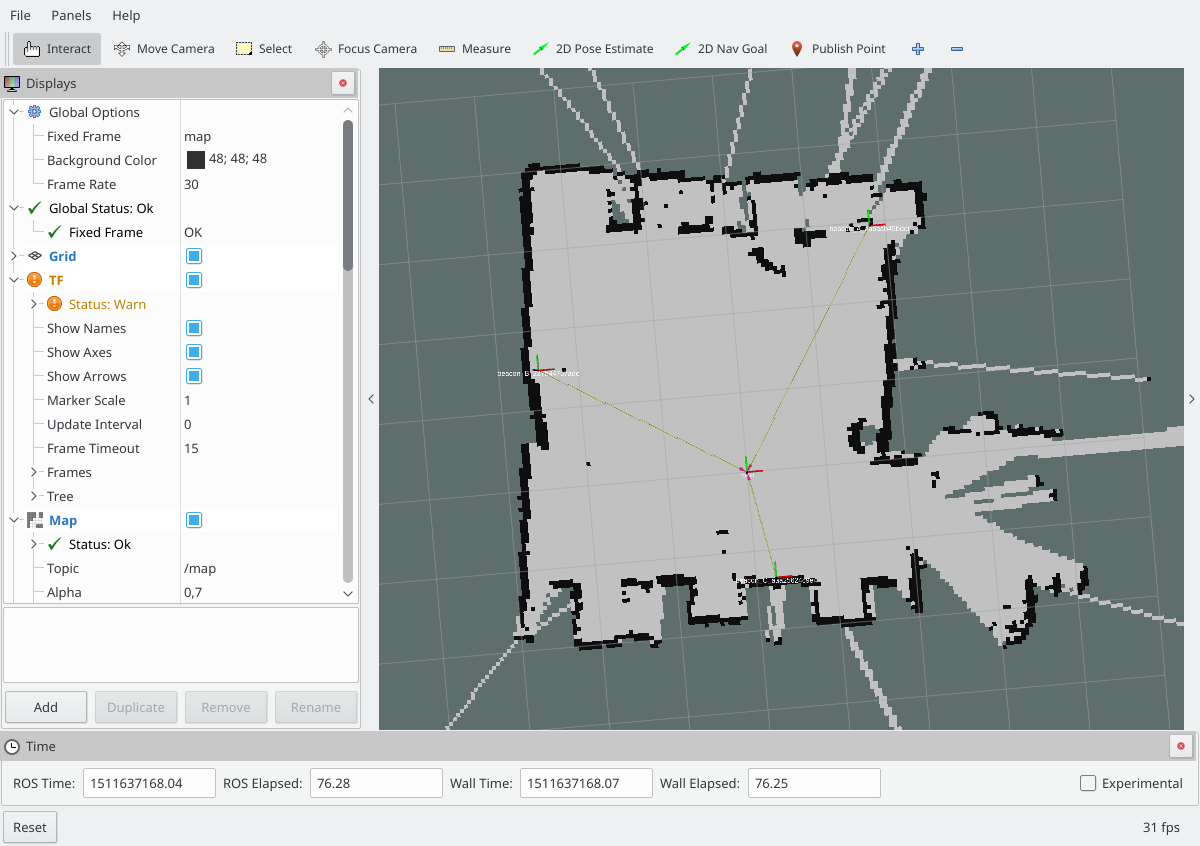
\includegraphics[width=0.8\textwidth]{img/rviz.png}
\caption{Okno programu RViz}
\label{fig:rviz}
\end{figure}

\subsubsection{Gmapping}
Gmapping jest narzędziem należącym do pakietu OpenSLAM, służącym do budowania dwuwymiarowych map pomieszczeń za pomocą SLAM (Simultaneous Localization And Mapping, ang. \textit{Jednoczesna Lokalizacja i Mapowanie}). Program wykorzystuje pomiar ze skanera laserowego oraz odometrię. 

\subsubsection{Rosbag}
Program Rosbag pozwala na zapisywanie do pliku danych publikowanych w wybranych tematach wraz z ich znacznikami czasowymi, celem późniejszego odtworzenia. Narzędzie to pozwoliło na nagranie szeregu testowych przejazdów robota, celem późniejszego zbudowania mapy pomieszczenia i wykonania pomiarów. Zaawansowane funkcjonalności manipulowania zegarem systemu ROS pozwalają na integrowanie danych odtwarzanych za pomocą Rosbag z danymi generowanymi w czasie rzeczywistym.

\subsubsection{Dodatkowe skrypty}
W ramach testów systemu przygotowano także szereg dodatkowych skryptów w języku Python:
\begin{itemize}
 \item skrypt do zbierania danych RSSI do pliku tekstowego, celem dalszej obróbki,
 \item skrypt do dopasowania modelu \ref{eq:logfit_d} do danych pomiarowych.
\end{itemize}


\section{Zmienność wartości siły sygnału RSSI}
\label{sec:zmiennosc}
\subsection{Metodyka badań}
Przedmiotem niniejszego eksperymentu było zbadanie przebiegu wartości RSSI w czasie dla sytuacji, w której nadajnik i odbiornik są nieruchome. Dodatkowo, wyznaczono histogramy wartości RSSI celem aproksymowania dystrybucji prawdopobieństwa wartości RSSI. 

Wykorzystano znacznik opisany w rozdziale \ref{subsec:znacznik} oraz odbiornik Wi-Fi/Bluetooth Intel 7260, zamontowany w laptopie Lenovo Y50 działającego pod kontrolą systemu Linux Mint 18. 

Testy przeprowadzono w pomieszczeniu o wymiarach 1.5 x 20 m (korytarz).Pomieszczenie to charakteryzował wysoki poziom zakłóceń radiowych w paśmie ISM (liczne punkty dostępowe Wi-Fi i odbiorniki elektryczne). Znacznik radiowy i odbiornik znajdowały się na wysokości 70 cm nad podłogą. Przeprowadzono pomiar dla odległości 1 m i 5 m. Pomiar polegał na zebraniu 100 wartości siły sygnału RSSI. Tak zebrane dane obrazowano w postaci wykresu czasowego i histogramu. 

\subsection{Wyniki}

Z wykresów \ref{fig:rssi-1m} i \ref{fig:rssi-5m} widać, że siła sygnału RSSI waha się znacznie nawet dla stanu ustalonego. Amplituda wahań dla odległości 1 m jest średnio rzędu 7 dBm. Dla odległości 5 m jest znacznie większa, rzędu 7 m. Stanowi to poważną przeszkodę dla pomiaru odległości za pomocą RSSI - kumulują się bowiem dwa negatywne czynniki: po pierwsze zależność RSSI od odległości jest w zakresie powyżej 2 m niemal płaska, po drugie - występują duże wahania wartości RSSI, które w tym zakresie będą się przekładać na znaczne wahania odległości. 

Wykresy \ref{fig:rssi-1m-hist} i \ref{fig:rssi-5m-hist} zawierają histogramy wygenerowane z danych pomiarowych. Dla odległości 1 m rozkład wyników pomiarów jest zbliżony do Gaussowskiego, jednak dla 5 m obserwujemy wyraźną asymetrię w kierunku niższych wartości siły sygnału. Jest to wynik wymienionych w rozdziale \ref{ch:radio} zakłóceń, szczególnie wielokrotnych odbić od ścian pomieszczenia. Także szerokość rozkładu jest większa niż w wypadku odległości 1 m. 

\begin{figure}[H]
\centering
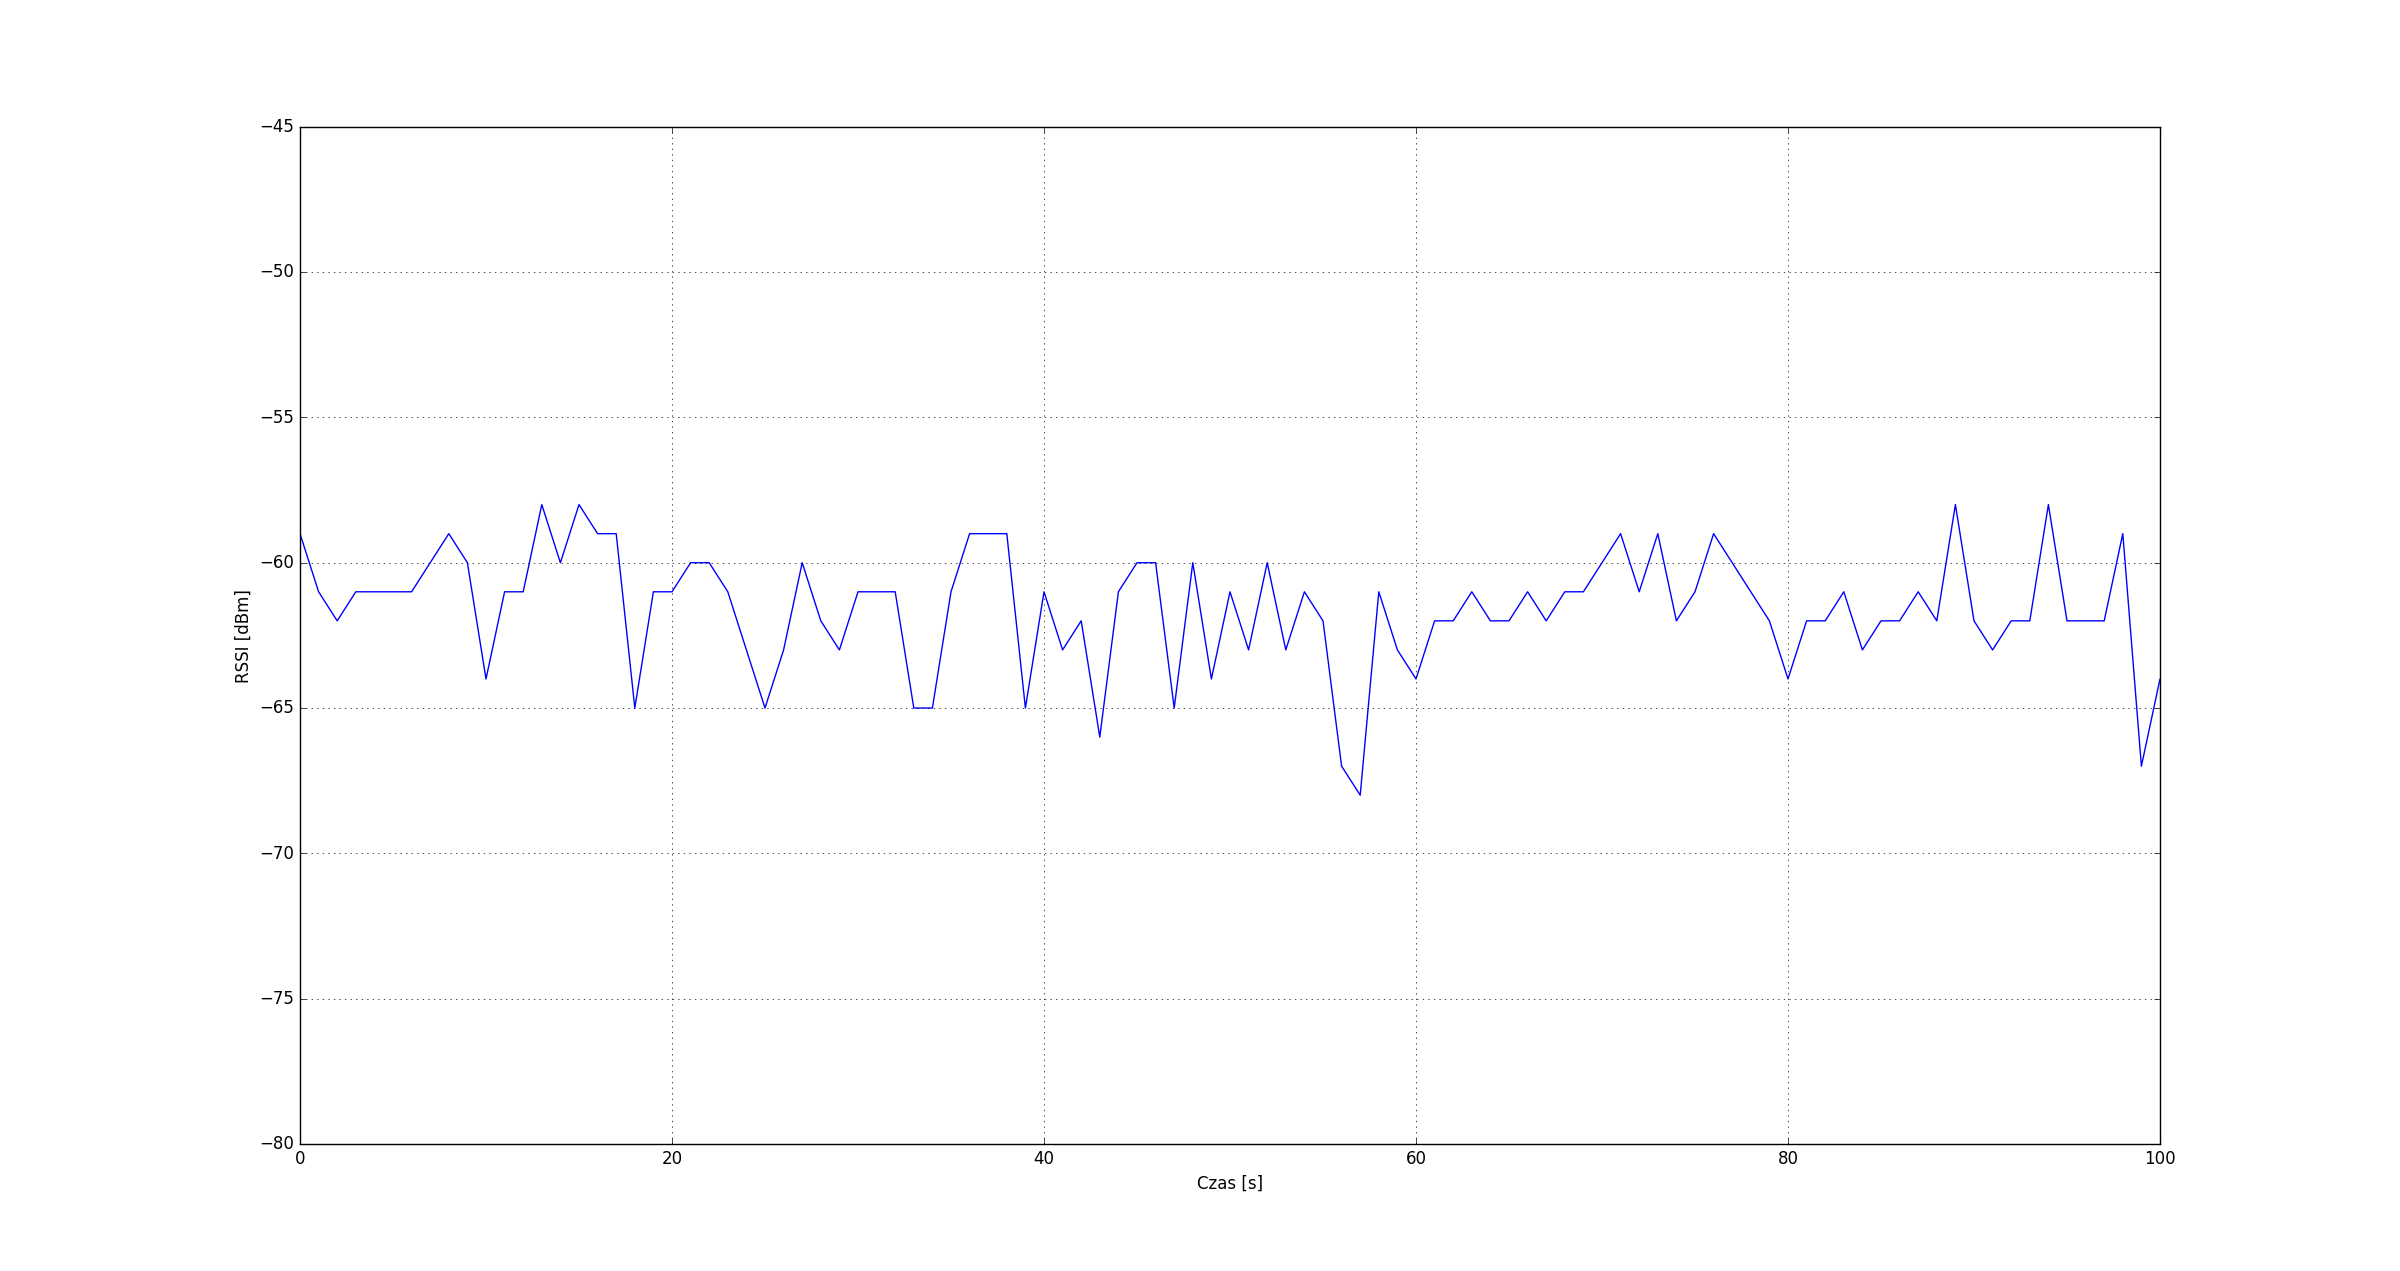
\includegraphics[width=1\textwidth]{img/1m.png}
\caption{Przebieg wartości siły sygnału RSSI w czasie dla odległości odbiornika od nadajnika równej 1 m}
\label{fig:rssi-1m}
\end{figure}

\begin{figure}[H]
\centering
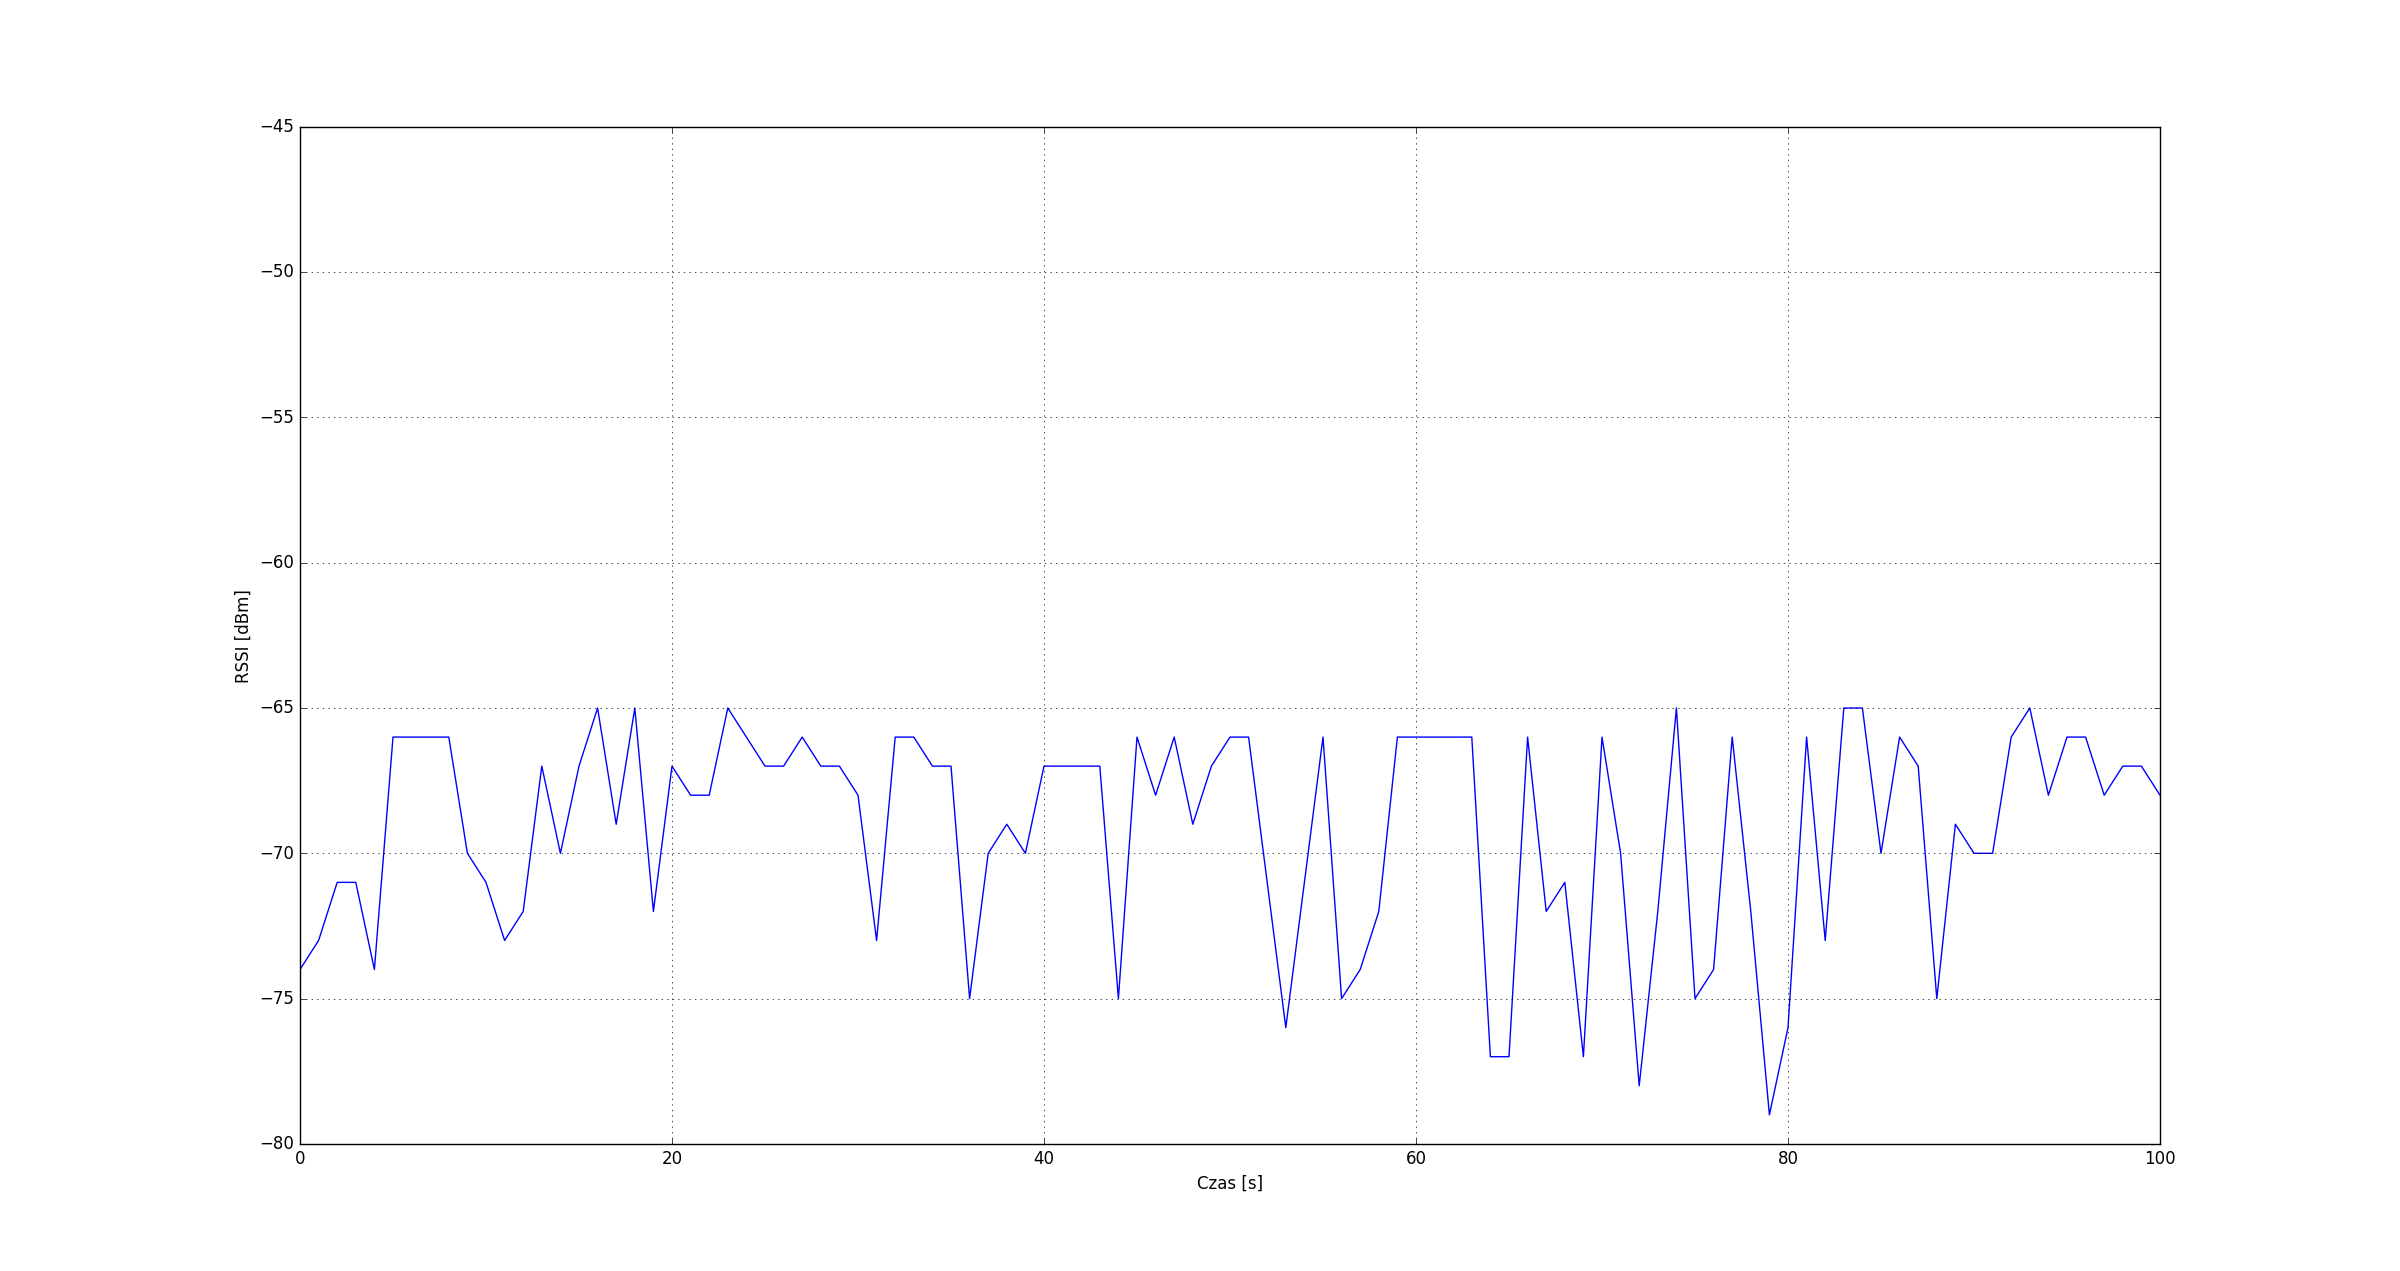
\includegraphics[width=1\textwidth]{img/5m.png}
\caption{Przebieg wartości siły sygnału RSSI w czasie dla odległości odbiornika od nadajnika równej 1 m}
\label{fig:rssi-5m}
\end{figure}

\begin{figure}[H]
\centering
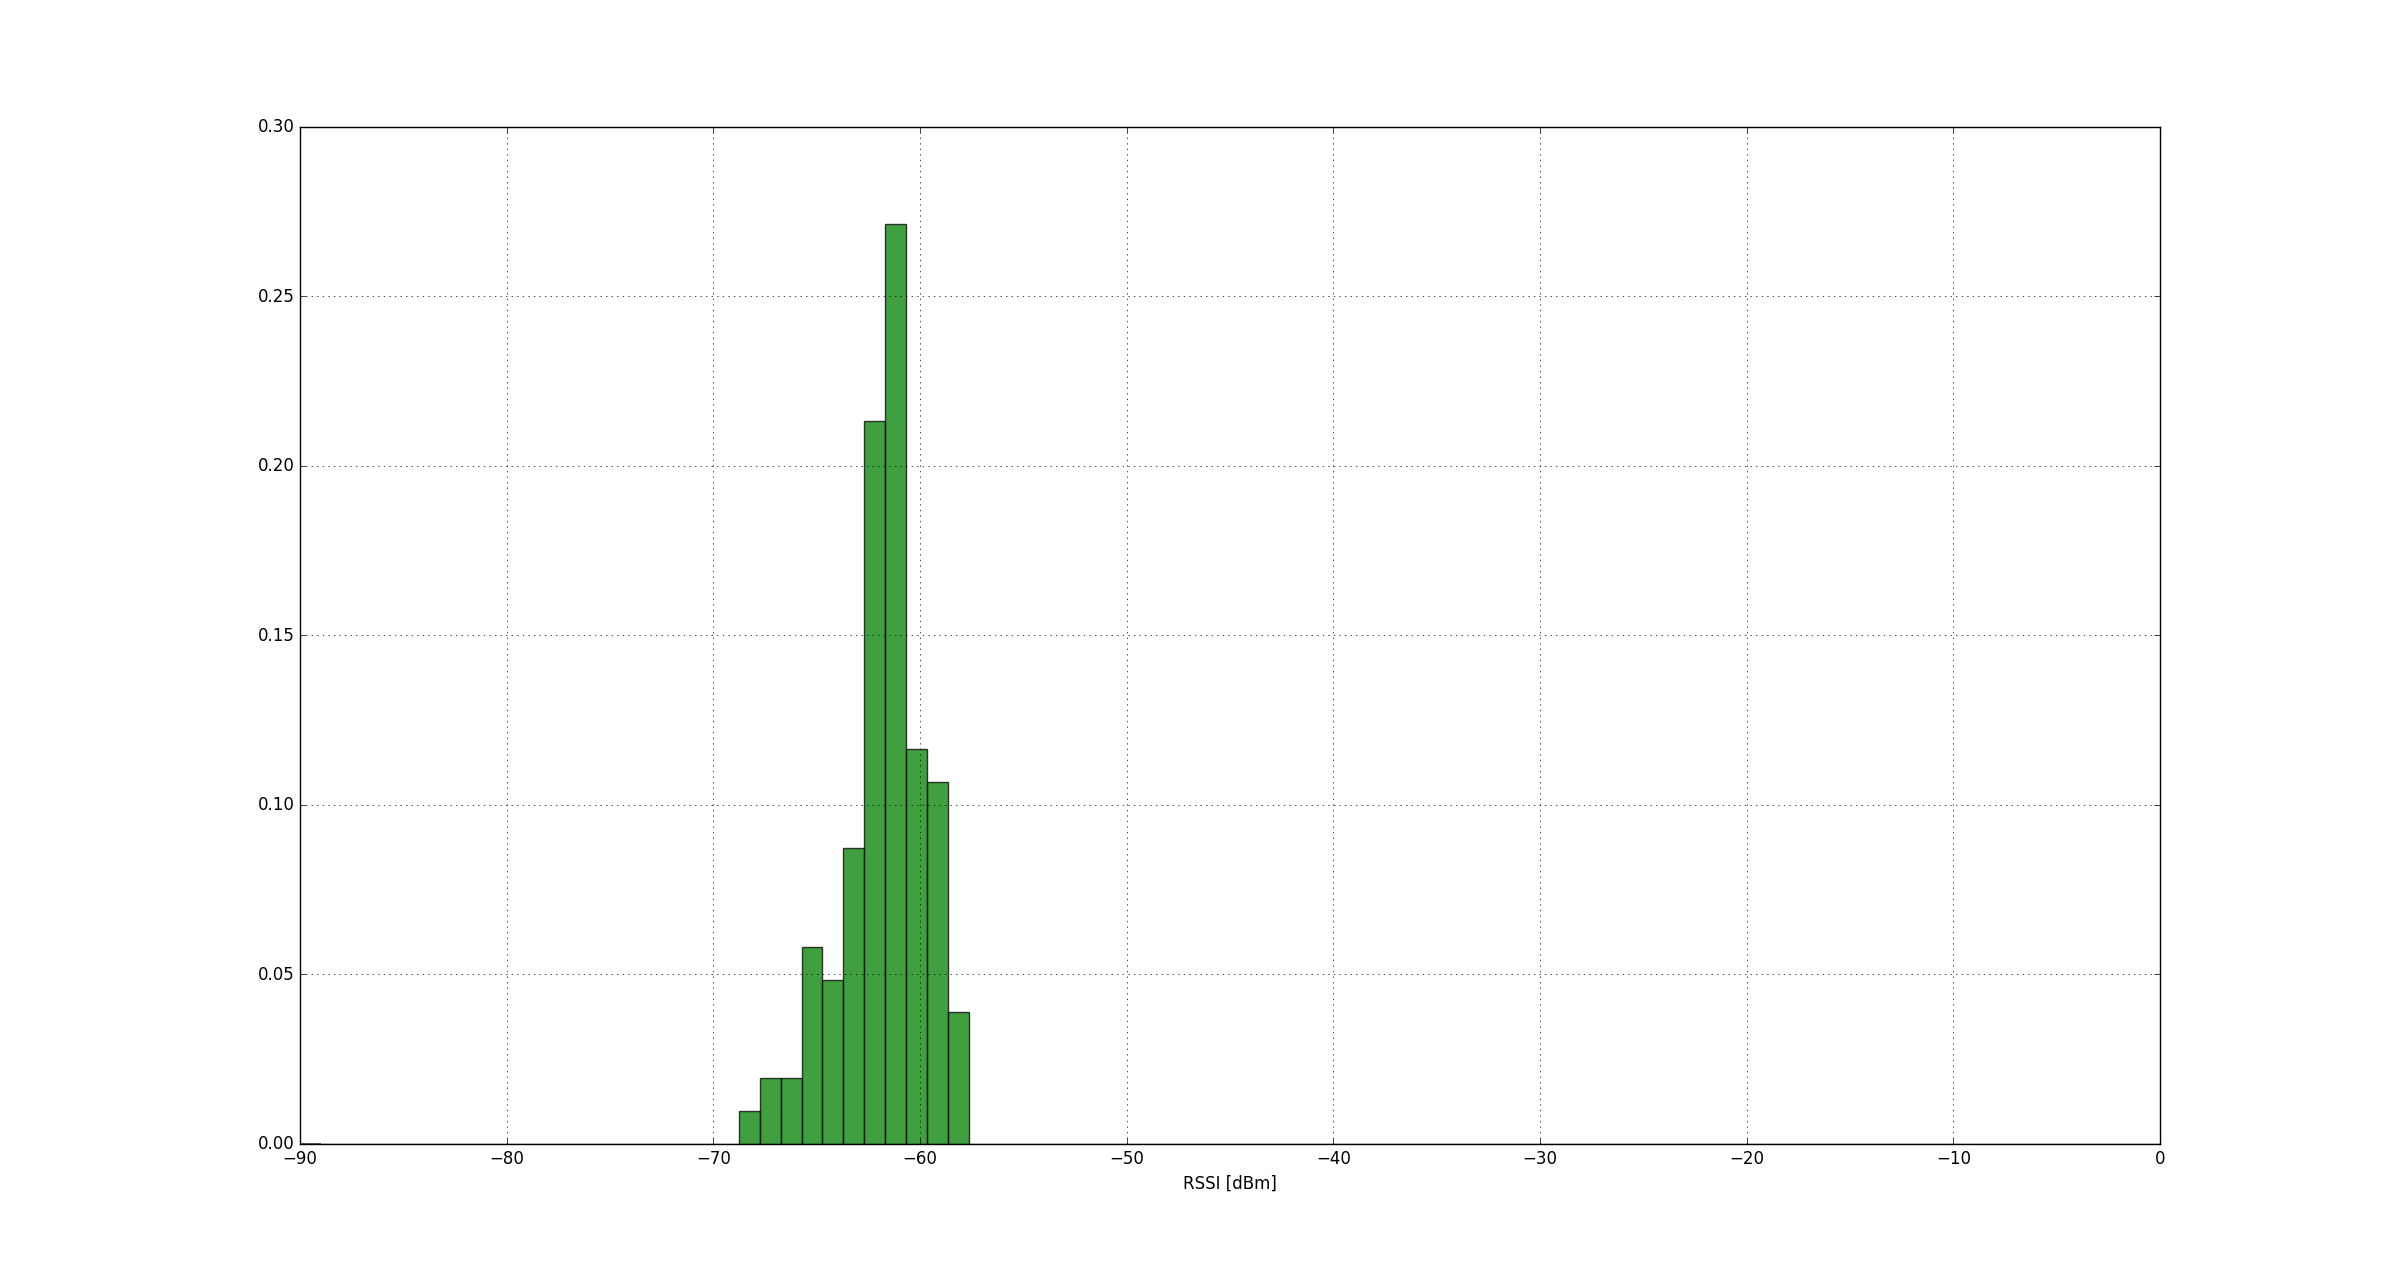
\includegraphics[width=1\textwidth]{img/1m-hist.png}
\caption{Histogram siły sygnału RSSI w czasie dla odległości odbiornika od nadajnika równej 1 m}
\label{fig:rssi-1m-hist}
\end{figure}

\begin{figure}[H]
\centering
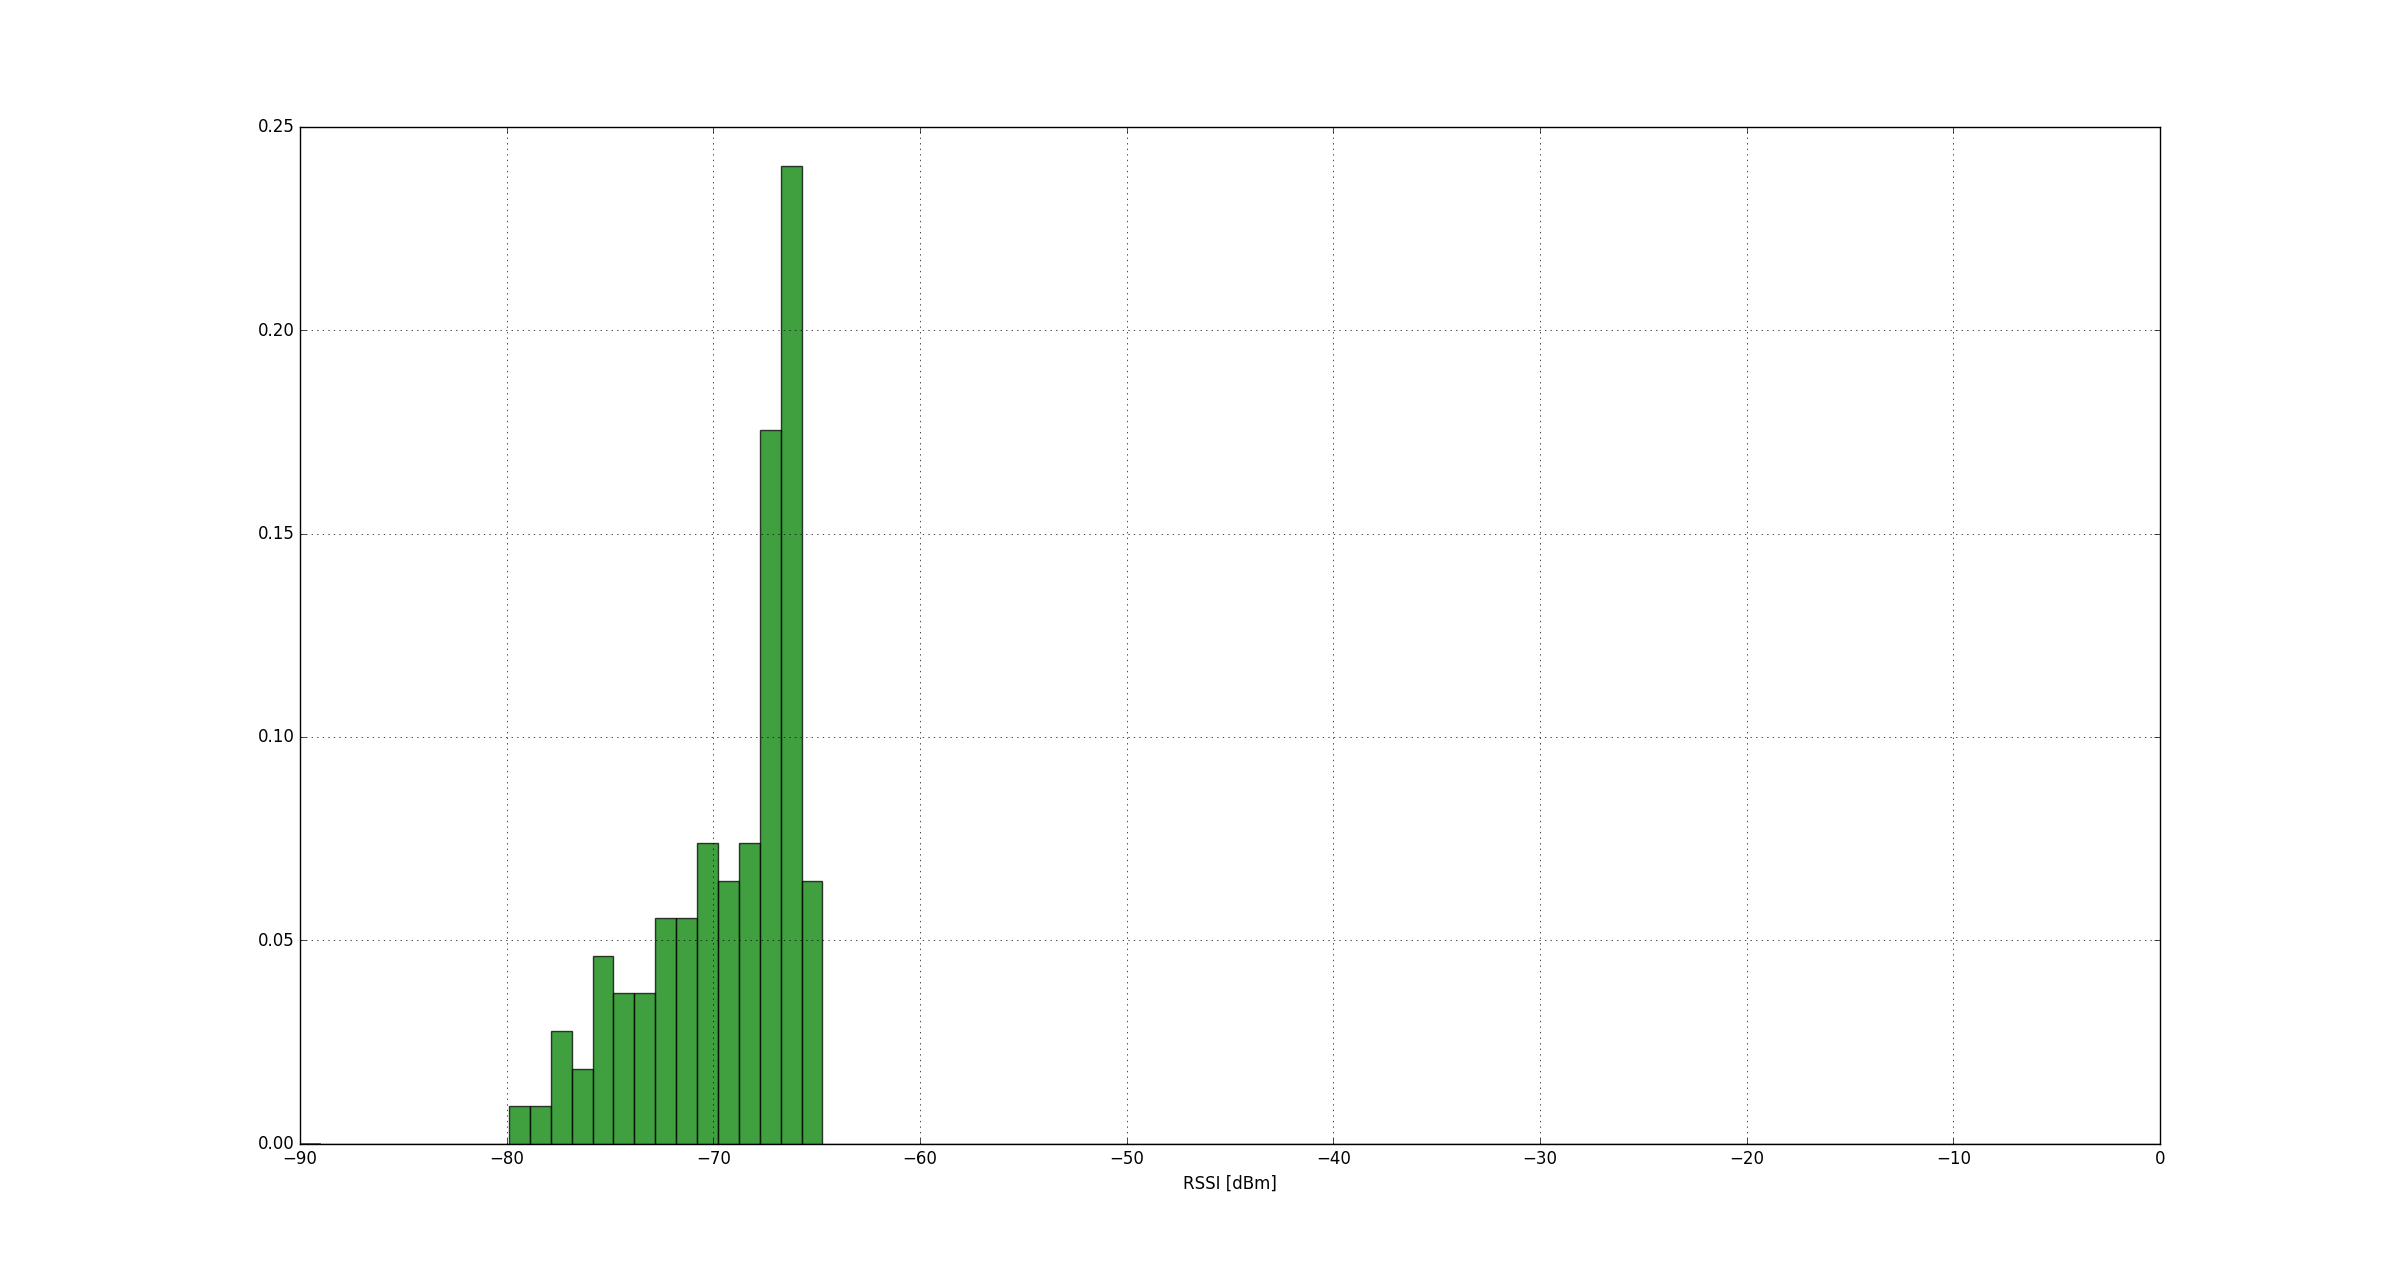
\includegraphics[width=1\textwidth]{img/5m-hist.png}
\caption{Histogram siły sygnału RSSI w czasie dla odległości odbiornika od nadajnika równej 1 m}
\label{fig:rssi-5m-hist}
\end{figure}


\section{Zależność siły sygnału RSSI od odległości}

\subsection{Metodyka badań}
Celem niniejszego eksperymentu jest zweryfikowanie modelu przedstawionego w rozdziale \ref{ch:radio}. Środowisko testowe było identyczne jak w punkcie \ref{sec:zmiennosc}. W każdym punkcie pomiarowym zebrano 30 próbek RSSI, które następnie uśredniono i wyznaczono odchylenie standardowe. Następnie wykonano dopasowanie krzywych logarytmicznych według metody interpolacji oraz dopasowania krzywej (por. rozdział \ref{sec:rssi-odleglosc}).

\subsection{Wyniki}

Na wykresie \ref{fig:odleglosc-rssi} widać logarytmiczną zależność pomiędzy odległością, a wartością siły sygnału RSSI, zgodną z oczekiwaniami teoretycznymi opisanymi w \ref{eq:model_propag}. Jednocześnie wraz ze wzrostem odległości od nadajnika, wzrasta odchylenie standardowe pomiarów, co oznacza że wahania wartości RSSI były większe. 

W odległości 3.5m oraz 5 m obserwujemy niewielki wzrost siły sygnału RSSI, co może wskazywać, że w tych miejscach środowiska testowego zachodziły warunki powodujące lokalne wzmocnienie fali. 
Należy zwrócić uwagę, iż w zakresie odległości powyżej 2 m wartość RSSI pozostaje na stałym poziomie, wahając się w granicach 10 dBm. Z tego powodu jakość pomiaru odległości za pomocą RSSI w tym zakresie będzie bardzo słaba. 

Wykres \ref{fig:odleglosc-rssi-fit} ukazuje dopasowane do wyników pomiaru krzywe: metodą interpolacji (\ref{eq:interpol}) i poprzez dopasowanie krzywej \ref{eq:logfit_d} za pomocą funkcji \textit{curve{\_}fit} z bilbioteki \textit{scipy} dla języka Python. Należy zwrócić uwage, iż w porównaniu z wykresem \ref{fig:odleglosc-rssi} zamienione zostały osie układu współrzędnych, tj. wykres \ref{fig:odleglosc-rssi-fit} przedstawia problem z perspektywy przeliczania RSSI na odleglość. 

Funkcja \textit{curve{\_}fit} uwzględnia wszystkie punkty pomiarowe wraz z ich niepewnościami, dlatego zapewnia lepsze dopasowanie od interpolacji, biorącej pod uwagę tylko dwa punkty pomiarowe. Jednakże, aby osiągnąć zadowalające dopasowanie, trzeba albo ręcznie wybrać dwa optymalne punkty do dopasowania interpolacyjnego, albo usunąć punkty zbyt odstające od pozostałych dla metody dopasowania krzywej. 

\begin{figure}[ht]
\centering
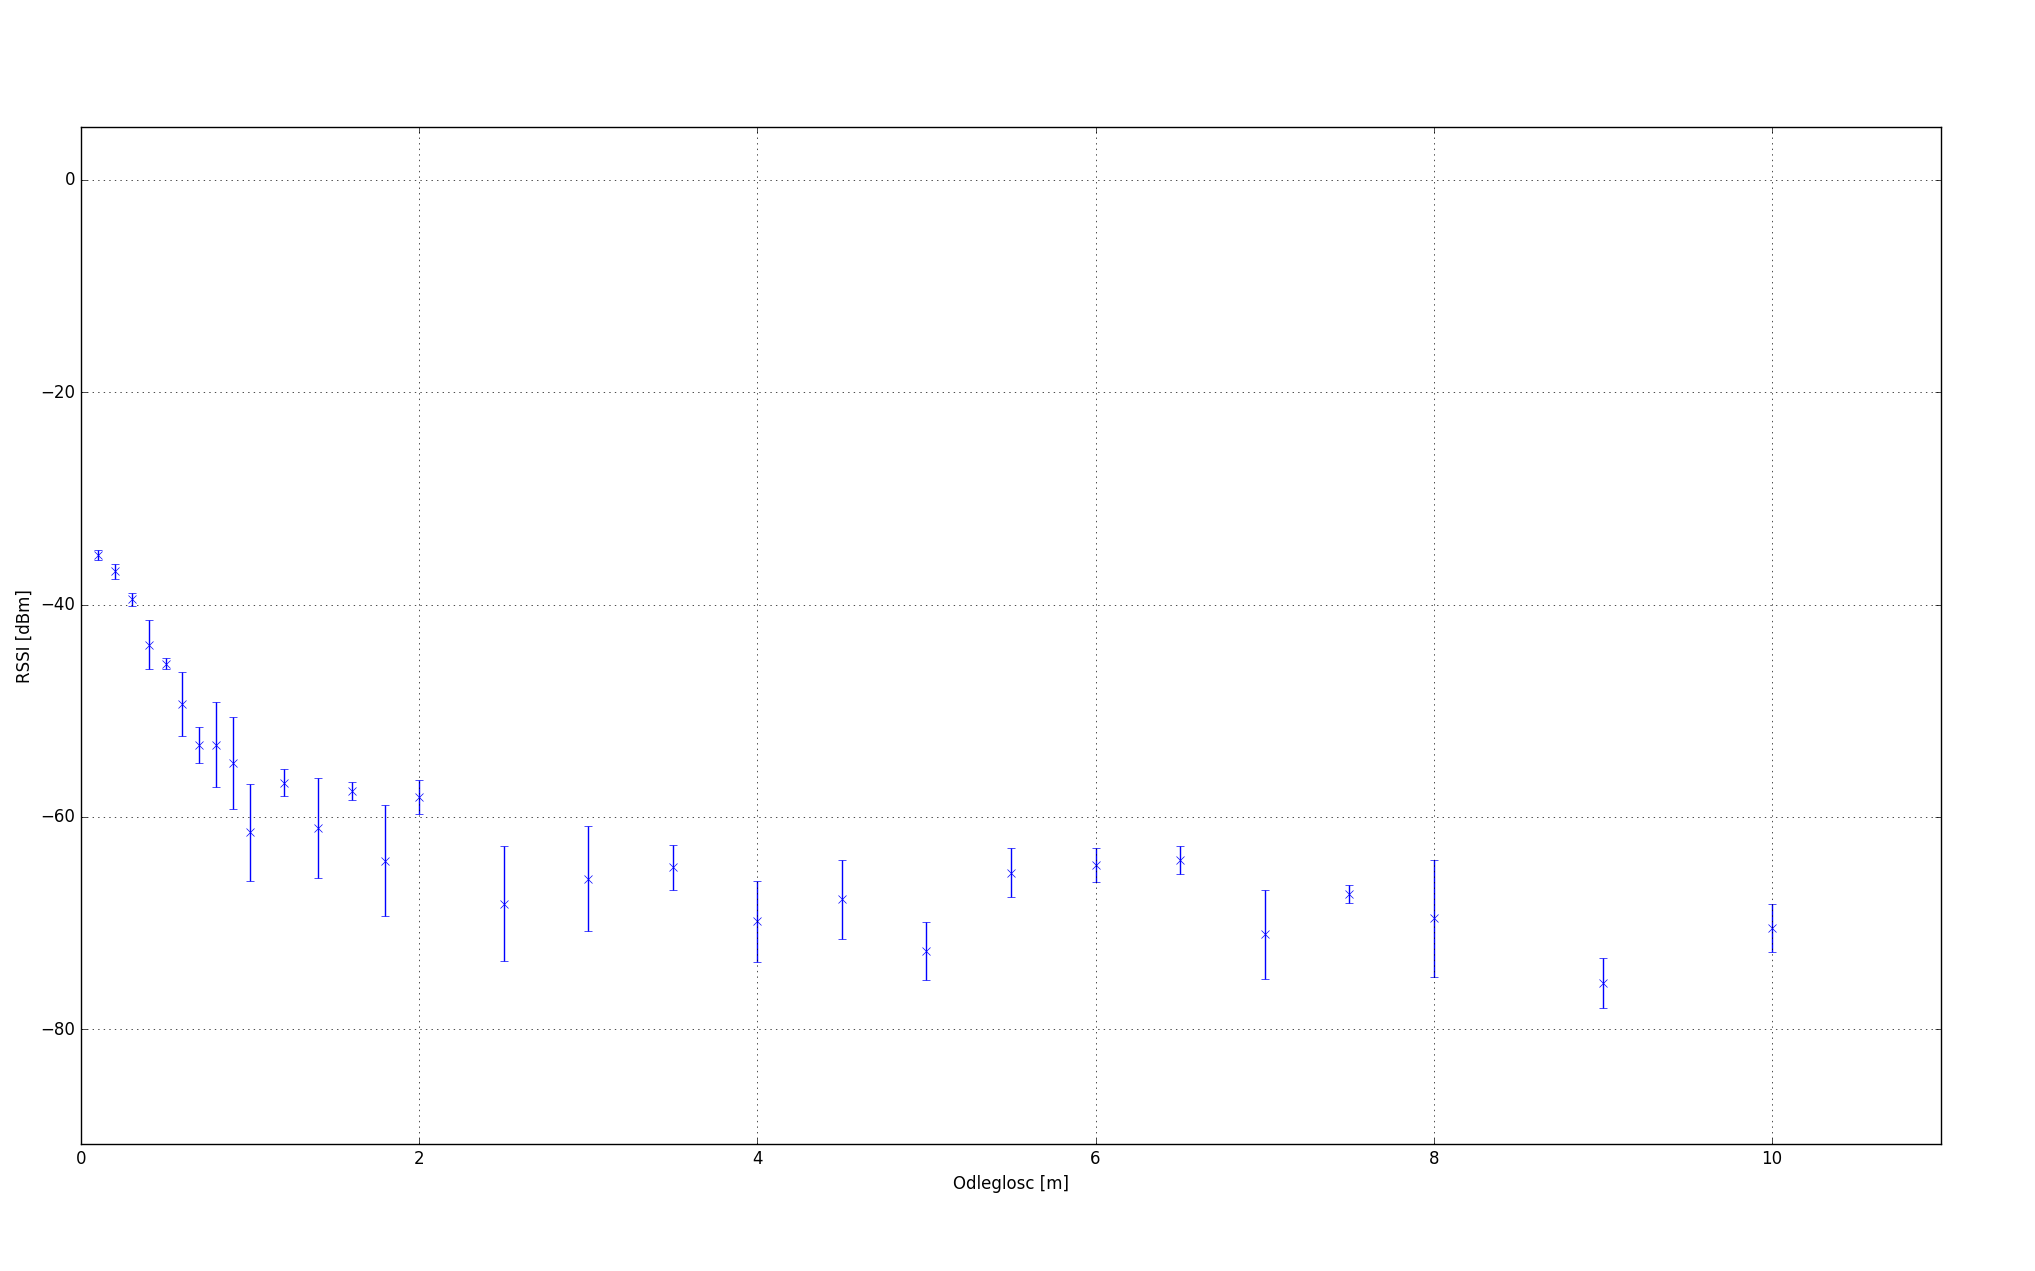
\includegraphics[width=1\textwidth]{img/odleglosc-rssi.png}
\caption{Wykres wartości siły sygnału RSSI w zależności odległości}
\label{fig:odleglosc-rssi}
\end{figure}


\begin{figure}[ht]
\centering
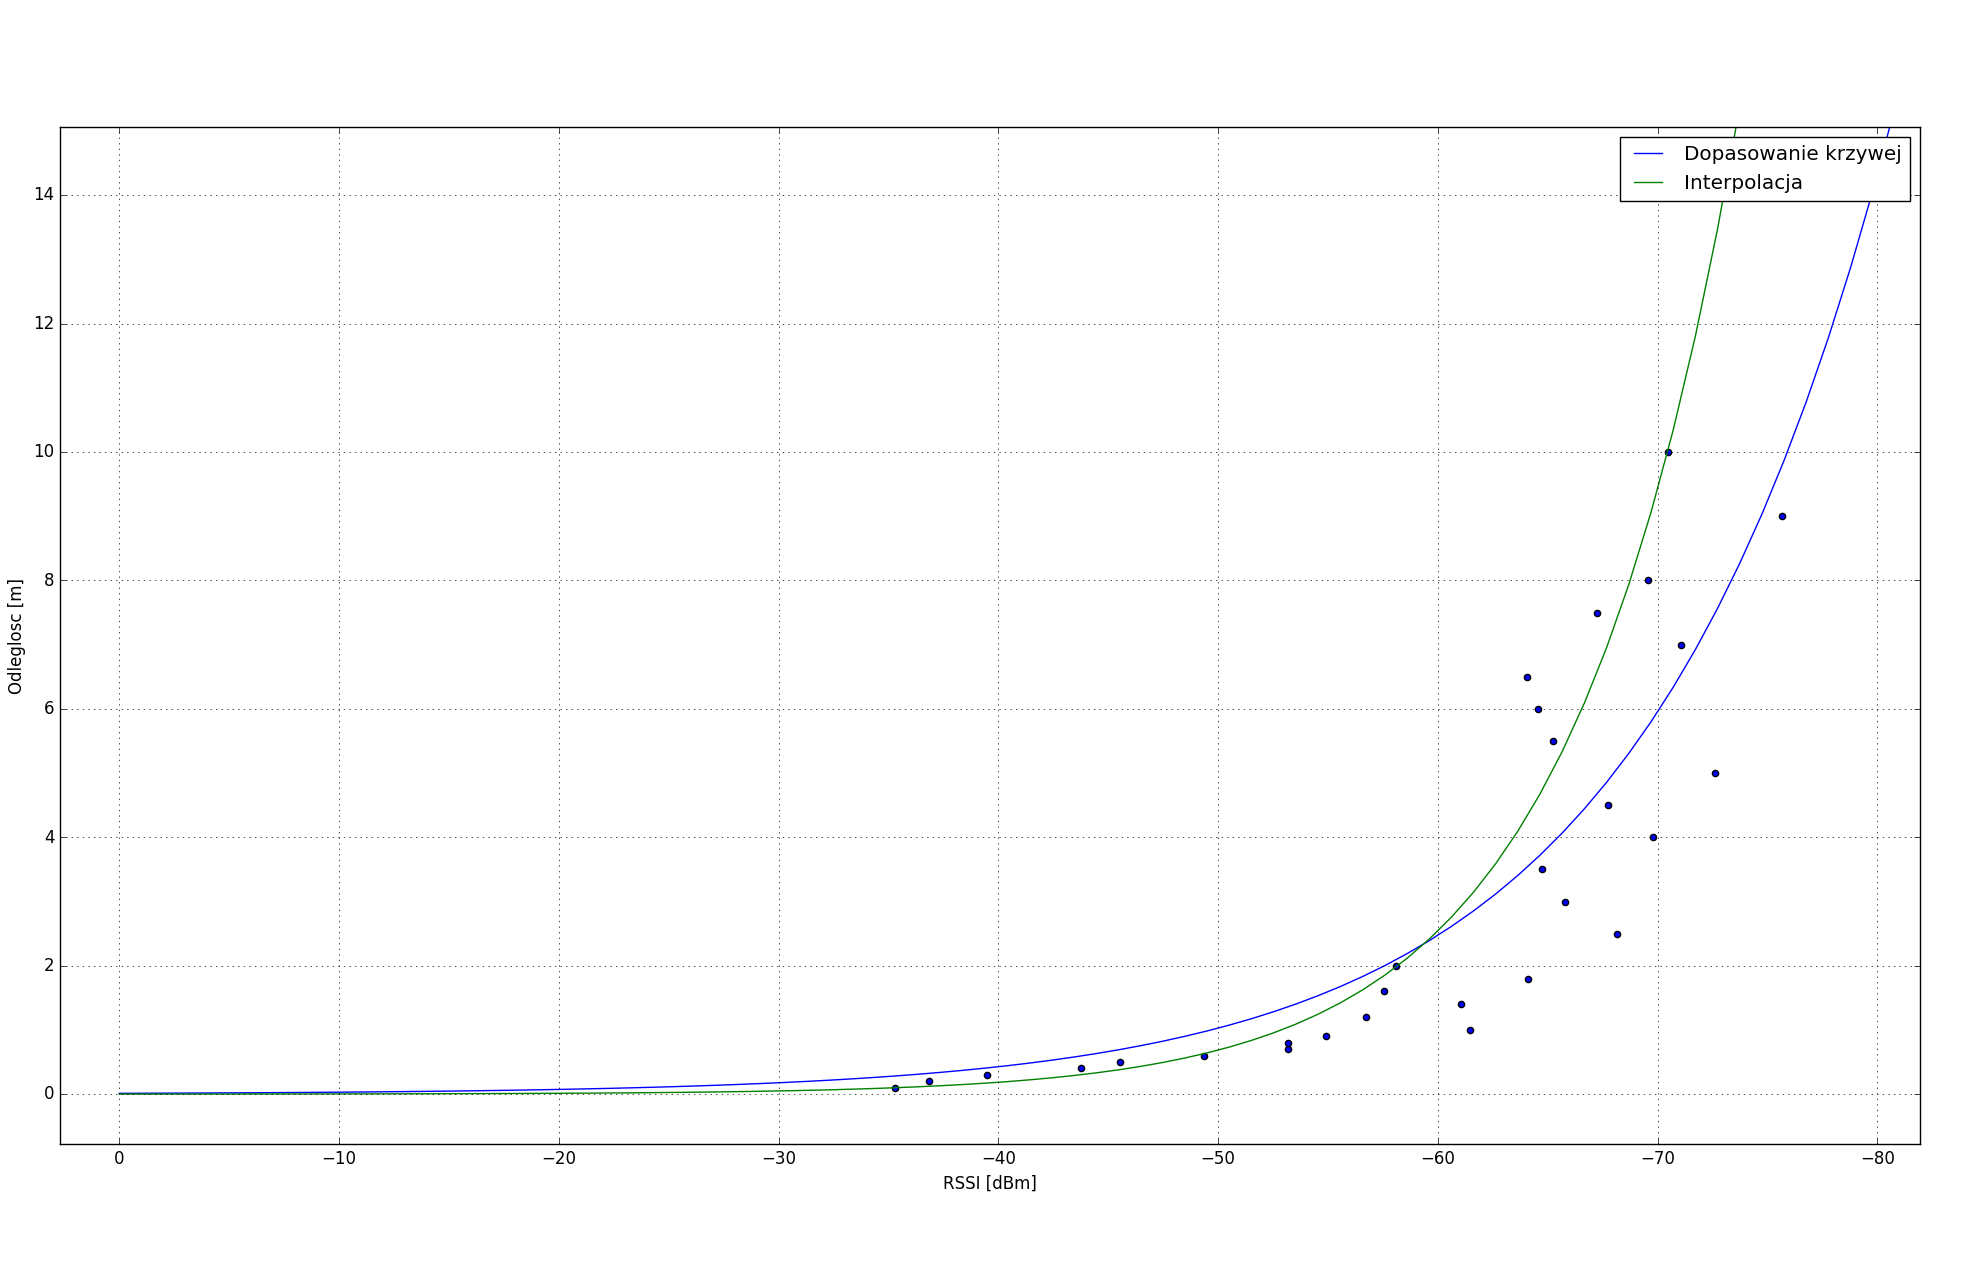
\includegraphics[width=1\textwidth]{img/rssi-odleglosc.png}
\caption{Wykres dopasowania krzywych potęgowych do wyników pomiaru}
\label{fig:odleglosc-rssi-fit}
\end{figure}

\section{Porównanie metod filtracji siły sygnału RSSI}
\label{sec:testy-filtracja}
\subsection{Metodyka badań}
Eksperyment miał na celu porównanie skuteczności metod filtracji sygnału RSSI opisanych w \ref{sec:rssi-odleglosc}. Pożądanym wynikiem jest dobre wygładzenie stacjonarnych wahań RSSI przy zachowaniu małej bezwładności, tj. szybkiej reakcji na rzeczywistą zmianę siły sygnału RSSI, wynikłą ze zmiany odległości od znacznika. 

W ramach eksperymentu posłużono się zbiorem danych nagranym za pomocą programu rosbag. Obejmował on pomiary RSSI zbierane z interwałem 1 sekundy, dla następującej sekwencji: przez 40 sekund znacznik pozostaje w odległości 1 m od odbiornika, następnie zostaje przeniesiony na odległość 2 m, po kolejnych 20 sekundach zostaje przeniesiony z powrotem na odległość 1 m gdzie pozostaje przez 40 sekund. 

\subsection{Wyniki}
Filtr średniej ruchomej (por. \ref{subsec:filtracja_rssi}) wprowadza znaczną bezwładność do układu (por. rys \ref{fig:filtry-avg}), przy czym dla większej liczby kroków średniej $N = 10$ bezwładność nie jest znacząco większa. Filtr zapewnia dobre wygładzenie dla nieruchomego odbiornika. W wypadku zmiany odgległości, filtr potrzebuje 10 sekund aby dość do stanu ustalonego, co dyskwalifikuje jego zastosowanie w lokalizacji dynamicznej. 

\begin{figure}[ht]
\centering
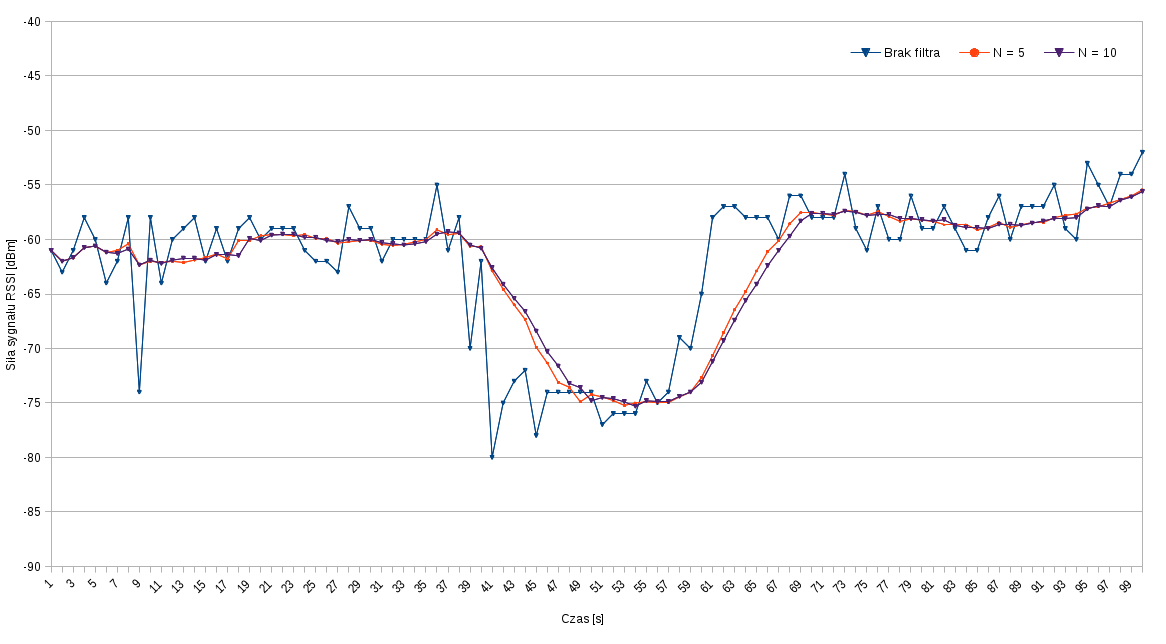
\includegraphics[width=0.9\textwidth]{img/filtr-avb.png}
\caption{Filtr średniej ruchomej}
\label{fig:filtry-avg}
\end{figure}

Filtr probablistyczny jest strojony za pomocą dwóch parametrów: $a$ - opisujący jak istotna jest wartość poprzedniego pomiaru w estymacji bieżącego, oraz $b$ - opisujący jak istotny jest przyrost wartości RSSI. Innymi słowy, parametr $a$ opisuje wygładzanie filtra, zaś $b$ opisuje czułość na zmiany RSSI. Zbyt niska wartość $a$ powoduje dużą bezwładność filtra, z kolei wartość $a=1$ powoduje że wartość estymowana jest wartości zmierzonej. Zbyt duża wartość $b$ spowoduje oscylacje, a nawet utratę stabilności filtra. 

W eksperymencie porównano dwa zestawy nastaw filtra (rys. \ref{fig:filtry-probab}):
\begin{itemize}
 \item \textbf{Nastawy 1} $a=0.35$ $b=0.02$
 \item \textbf{Nastawy 2} $a=0.15$ $b=0.005$
\end{itemize}

Nastawy 2 zapewniają dobre wygładzenie w stanie ustalonym oraz bardzo dużą bezwładność. Zwiększanie parametru $b$ spowoduje jedynie zaistnienie oscylacji, bez poprawy reakcji filtra. 

Z kolei nastawy 1 stanowią dobry kompromis pomiędzy wygładzeniem a reakcją na zmiany RSSI. Filtr reaguje na zmianę odległości w ciągu około 4 sekund, zaś amplituda wahań wartości w stanie ustalonym jest rzędu 3 dBm. 
\begin{figure}[ht]
\centering
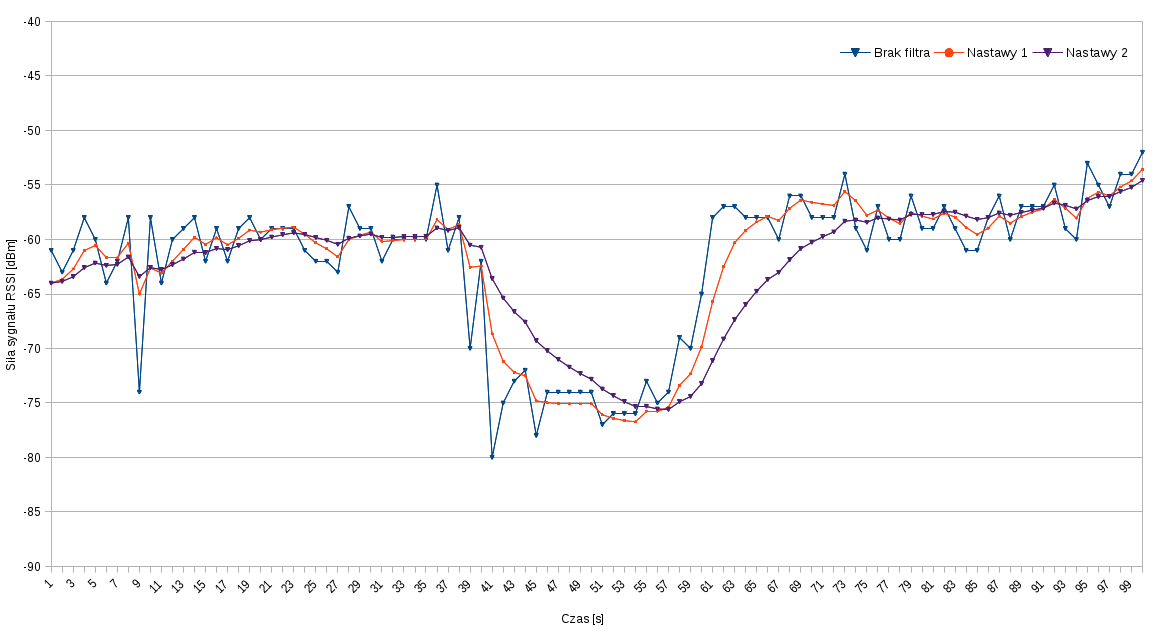
\includegraphics[width=0.9\textwidth]{img/filtr-propab.png}
\caption{Filtr probabilistyczny}
\label{fig:filtry-probab}
\end{figure}
Na wykresie \ref{fig:filtry-wszystkie} przedstawiono przebieg RSSI bez filtracji, z filtracją średnią ruchomą dla $N=5$ oraz filtracją probabilistyczną wg. nastaw 1. Filtr średniej ruchomej ma znacznie większą bezwładność od filtra probabilistycznego. Dlatego do testowania lokalizacji robota wykorzystano właśnie filtr probabilistyczny, jako lepiej radzący sobie w sytuacjach dynamiczych. 
\begin{figure}[H]
\centering
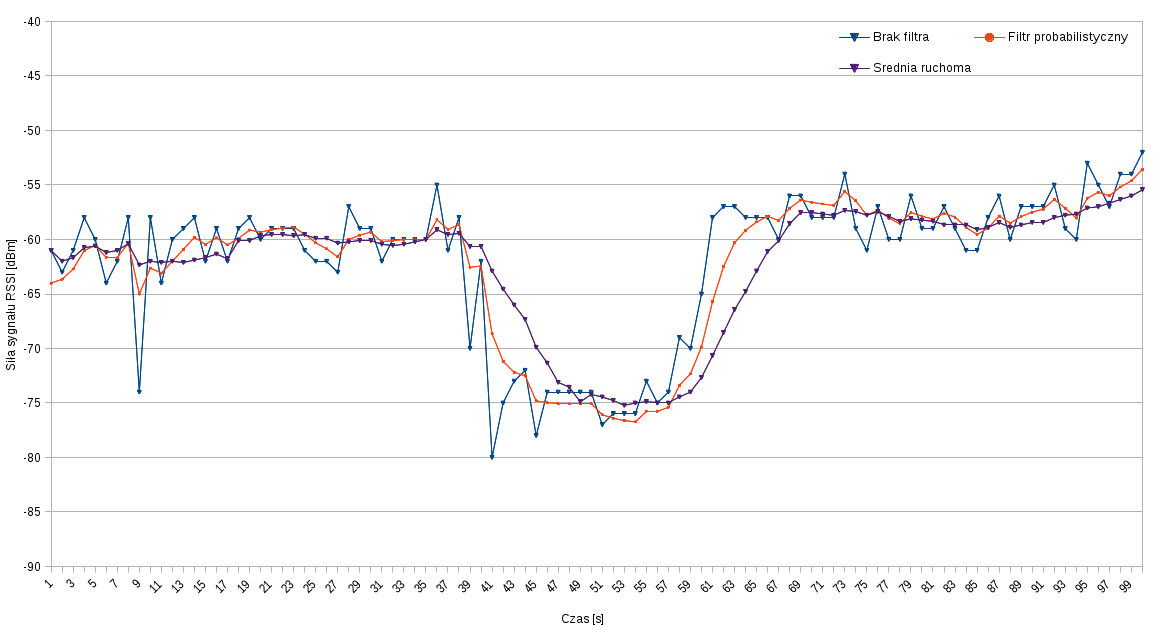
\includegraphics[width=0.9\textwidth]{img/filtry-porownanie.png}
\caption{Porównanie metod filtracji}
\label{fig:filtry-wszystkie}
\end{figure}

\section{Porównanie metod lokalizacji}
W niniejszej sekcji opisano przebieg i wyniki badania zasadniczej części niniejszej pracy - algorytmu lokalizacji. W celu wykonania badań, konieczne było zbudowanie mapy środowiska pracy robota oraz skalibrowanie znaczników, tj. wyznaczenie parametrów modelu \ref{eq:logfit_d}. 
\subsection{Metodyka badań}
Badania metod lokalizacji przeprowadzono na opisanym w rozdziale \ref{sec:hardware} robocie Pioneer 3-AT, w pomieszczeniu Laboratorium Robotyki Mobilnej Wydziału Mechatroniki PW. Do zbudowania mapy pomieszczenia, potrzebnej do pomiarów, wykorzystano program Gmapping. Budowanie mapy polegało na wykonaniu 3 przejazdów dookoła pomieszczenia. W trakcie przejazdów unikano gwałtownych przyspieszeń, hamowań i skrętów robota, w celu ograniczenia uślizgu kół, który wprowadza błąd do mapowania SLAM. 
Tak wyznaczoną mapę zapisano w pliku graficznym PNG. Jeden piksel obrazka reprezentował 5 cm przestrzeni. Następnie zlokalizowano na mapie umiejscowienie znaczników, korzystając z punktów charakterystycznych. 

W celu skalibrowania znaczników zebrano szereg punktów pomiarowych w różnych odległościach od znacznika. Aby wyeliminować wpływ wahań RSSI na wyznaczony model, każdy pomiar składał się z 20 uśrednionionych wartości RSSI.  Następnie wyznaczono model w oparciu o interpolację i dopasowanie funkcji wykładniczej. 

Do badania metod lokalizacji jako odniesienie wykorzystano lokalizację AMCL. Po wykonaniu kilku przejazdów robota po pomieszczeniu oparta o filtr cząsteczkowy lokalizacja AMCL zapewnia dokładność zbliżoną do rozdzielczości mapy, co najmniej o rząd wielkości lepszą niż dokładność lokalizacji w oparciu o znaczniki. Aby zapewnić rzetelne porównanie metod lokalizacji, posłużono się danymi nagranymi programem Rosbag, zatem obydwie metody zostały użyte na identycznych danych testowych. 

W obydwu metodach porównano wyniki lokalizacji obliczone z odległości przefiltrowanych przez poszczególne filtry (por. \ref{sec:testy-filtracja}).
\subsection{Wyniki}

\subsubsection{Mapa środowiska}
Rysunek \ref{fig:mapa} przedstawia wyznaczoną metodą SLAM mapę laboratorium. Punkty w kolorze szarym oznaczają obszar wolny, zaś w kolorze czarnym - zajęty. Pojedyncze czarne punkty i szare linie stanowią wynik zakłóceń SLAM i nie mają negatywnego wpływu na lokalizację. Obszar w prawym dolnym rogu mapy obrazuje otwarte drzwi do sąsiedniego pomieszczenia, które nie było objęte mapowaniem. Na mapie zobrazowane są pozycje początków układów współrzędnych: mapy oraz 3 znaczników. 
\begin{figure}[H]
\centering
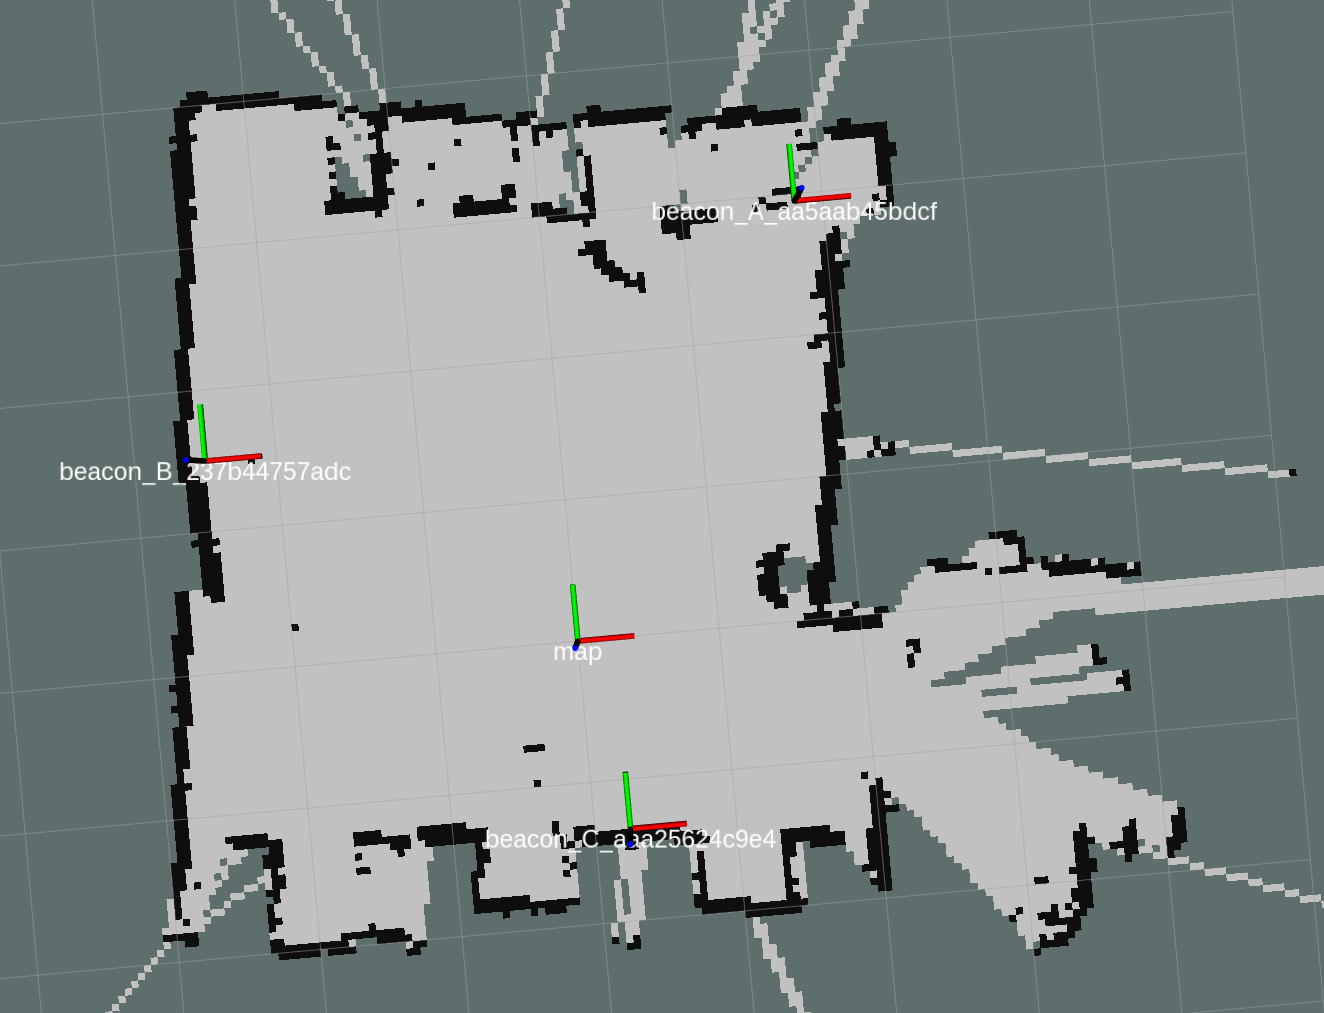
\includegraphics[width=0.9\textwidth]{img/mapa2.png}
\caption{Mapa środowiska wyznaczona metodą SLAM za pomocą programu GMapping z zaznaczonymi znacznikami radiowymi.}
\label{fig:mapa}
\end{figure}


\subsubsection{Kalibracja znaczników}

Tabela \ref{tab:strojenie} przedstawia wyniki kalibracji znaczników. Z wyników pomiaru usunięto punkty znacząco odbiegające od oczekiwanego przebiegu. Dopasowane krzywe wraz z punktami pomiarowymi wykreślono na rys. \ref{fig:strojenie-a}, \ref{fig:strojenie-b} oraz \ref{fig:strojenie-c}.

\begin{table}[H]
 \caption{Wyniki kalibracji}
 \label{tab:strojenie}
 \begin{tabular}{|l|l|l|}
  \hline
  \textbf{Znacznik}	& \textbf{Interpolacja} & \textbf{Dopasowanie krzywej potęgowej }\\ \hline
  A 		& $a=50,515$, $b=28,631$	& $a=50,167$, $b=28,480$	\\ \hline
  B 		& $a=65,036$, $b=11,547$	& $a=66,028$, $b=10,074$	\\ \hline
  C 		& $a=65,468$, $b=7,319$		& $a=68,215$, $b=0,984$		\\ \hline
 \end{tabular}

\end{table}


\begin{figure}[H]
\centering
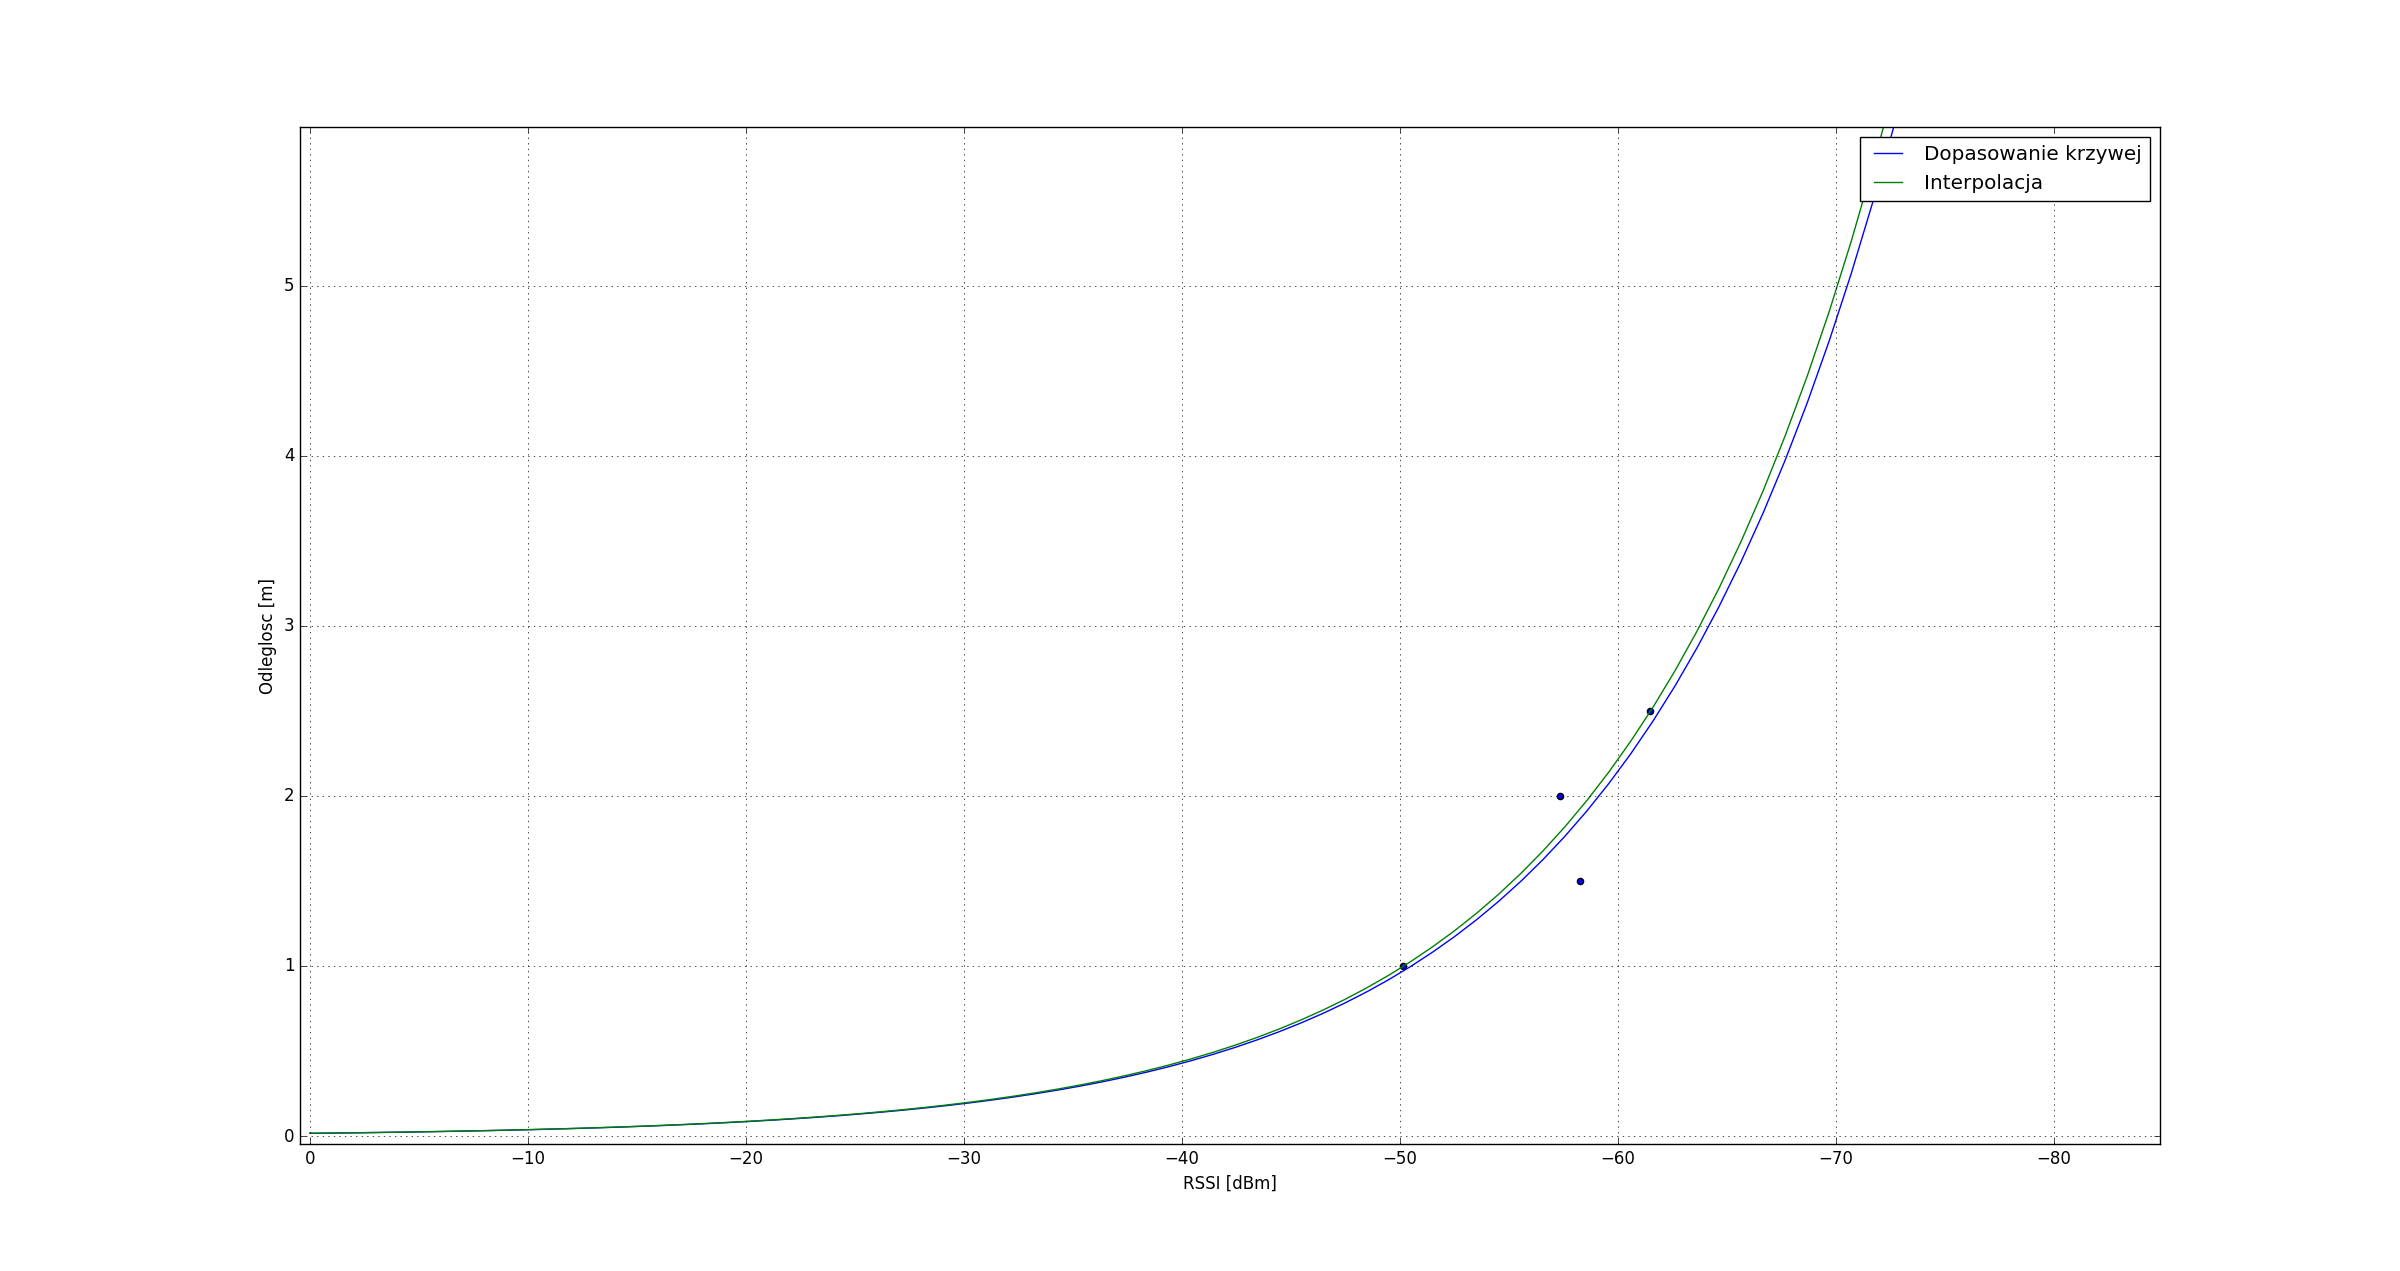
\includegraphics[width=1\textwidth]{img/strojenie-a.png}
\caption{Wyznaczanie modelu znacznika A}
\label{fig:strojenie-a}
\end{figure}

\begin{figure}[H]
\centering
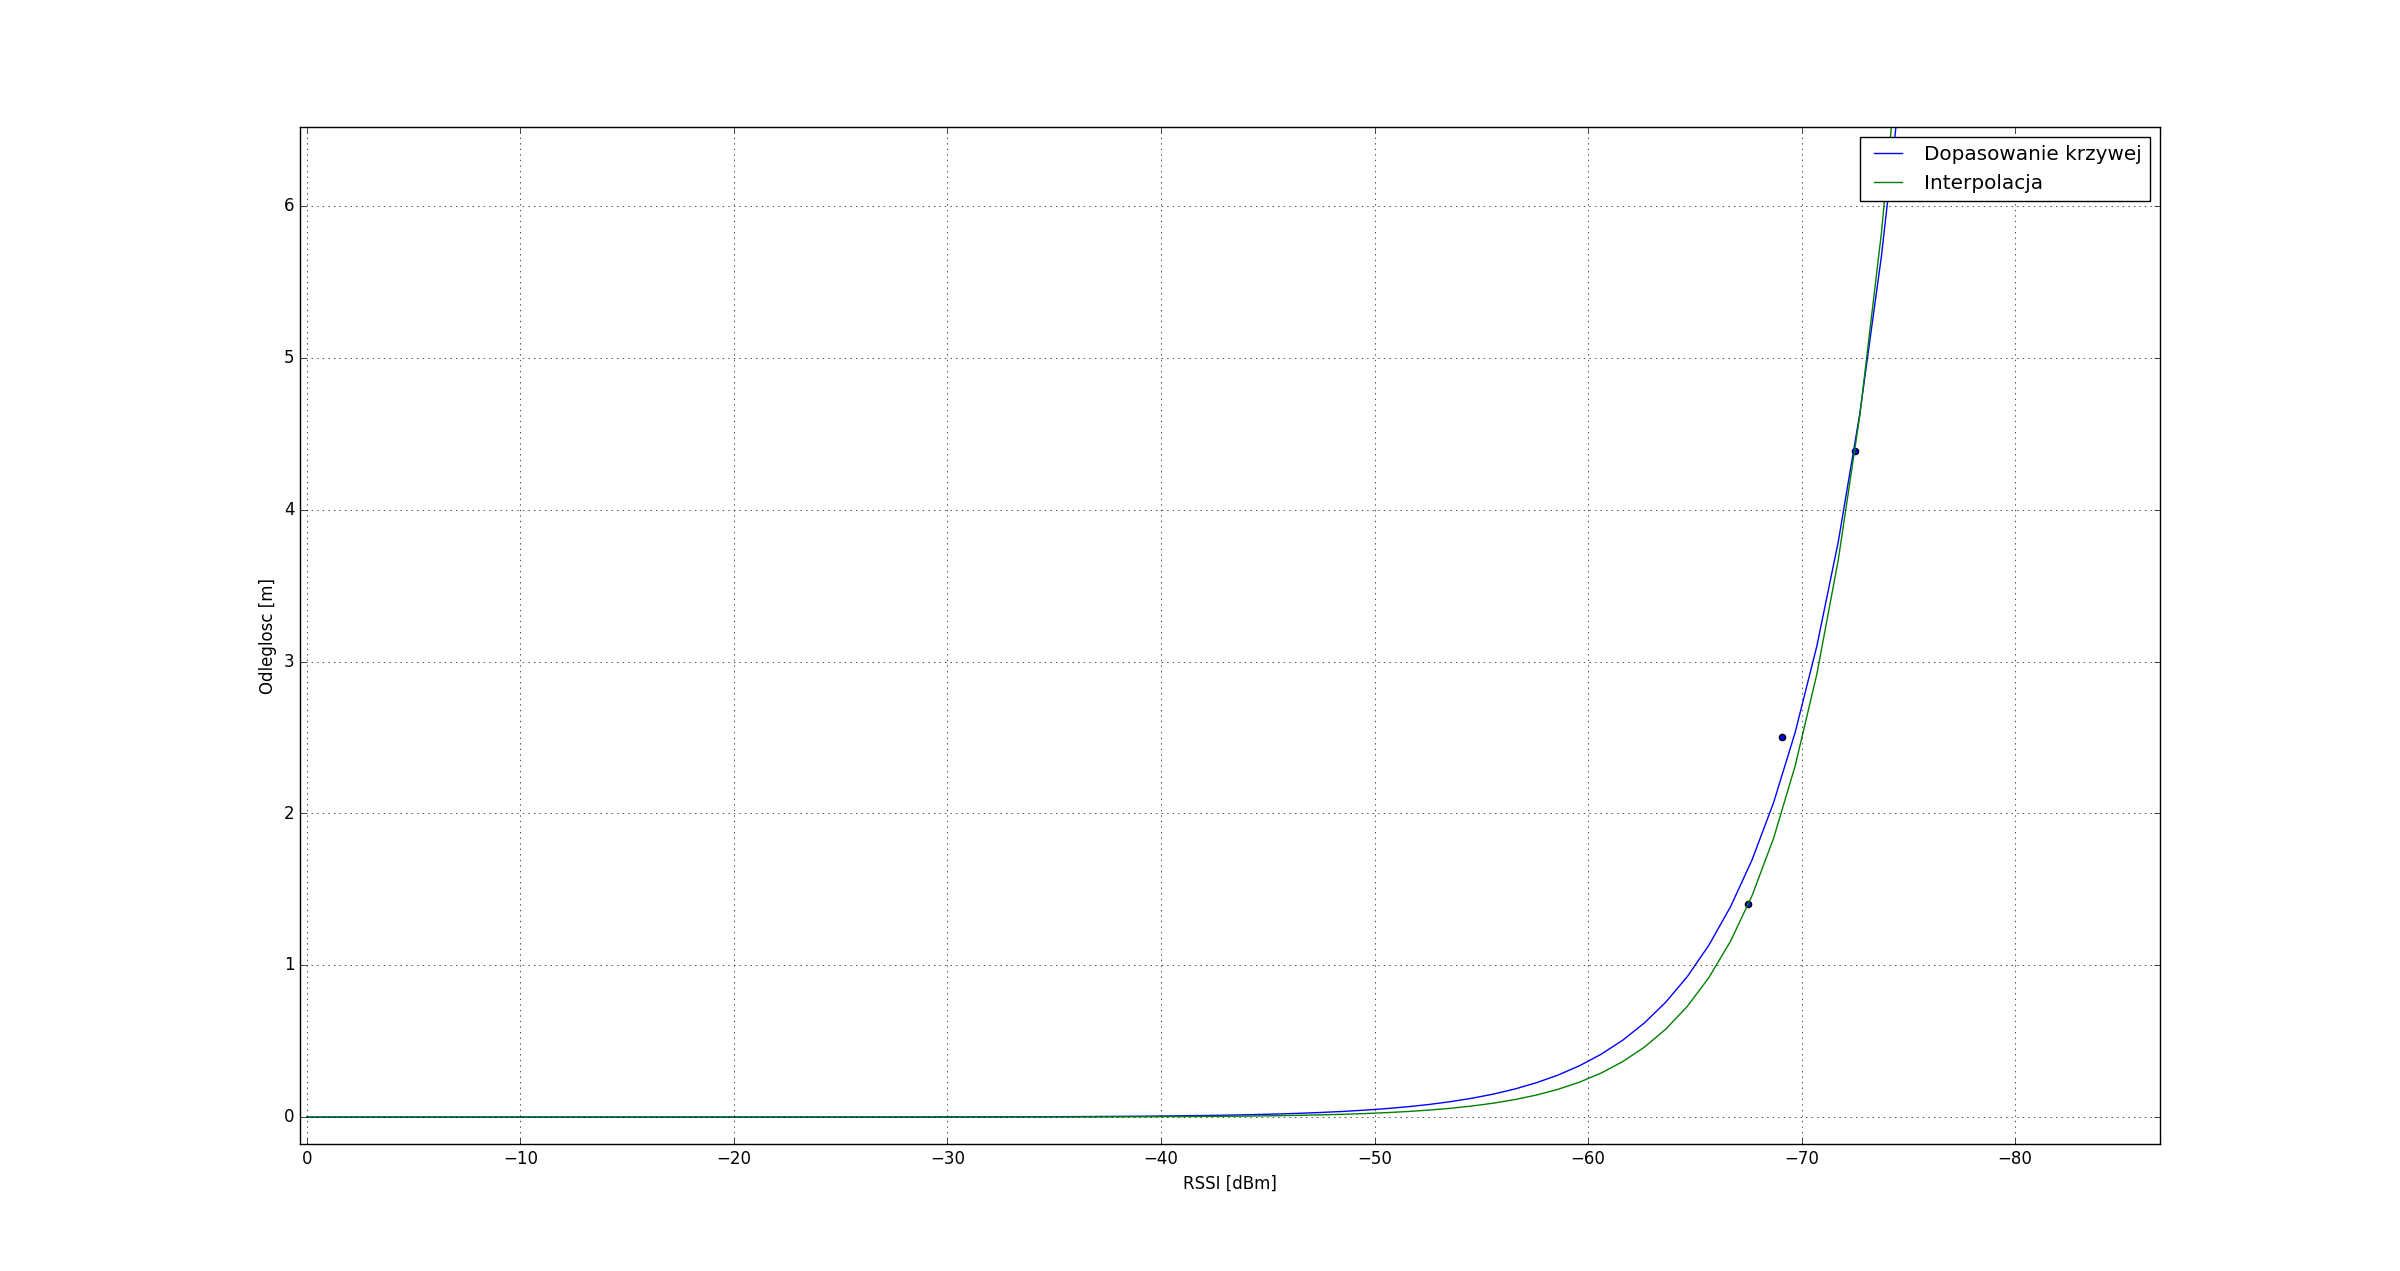
\includegraphics[width=1\textwidth]{img/strojenie-b.png}
\caption{Wyznaczanie modelu znacznika B}
\label{fig:strojenie-b}
\end{figure}

\begin{figure}[H]
\centering
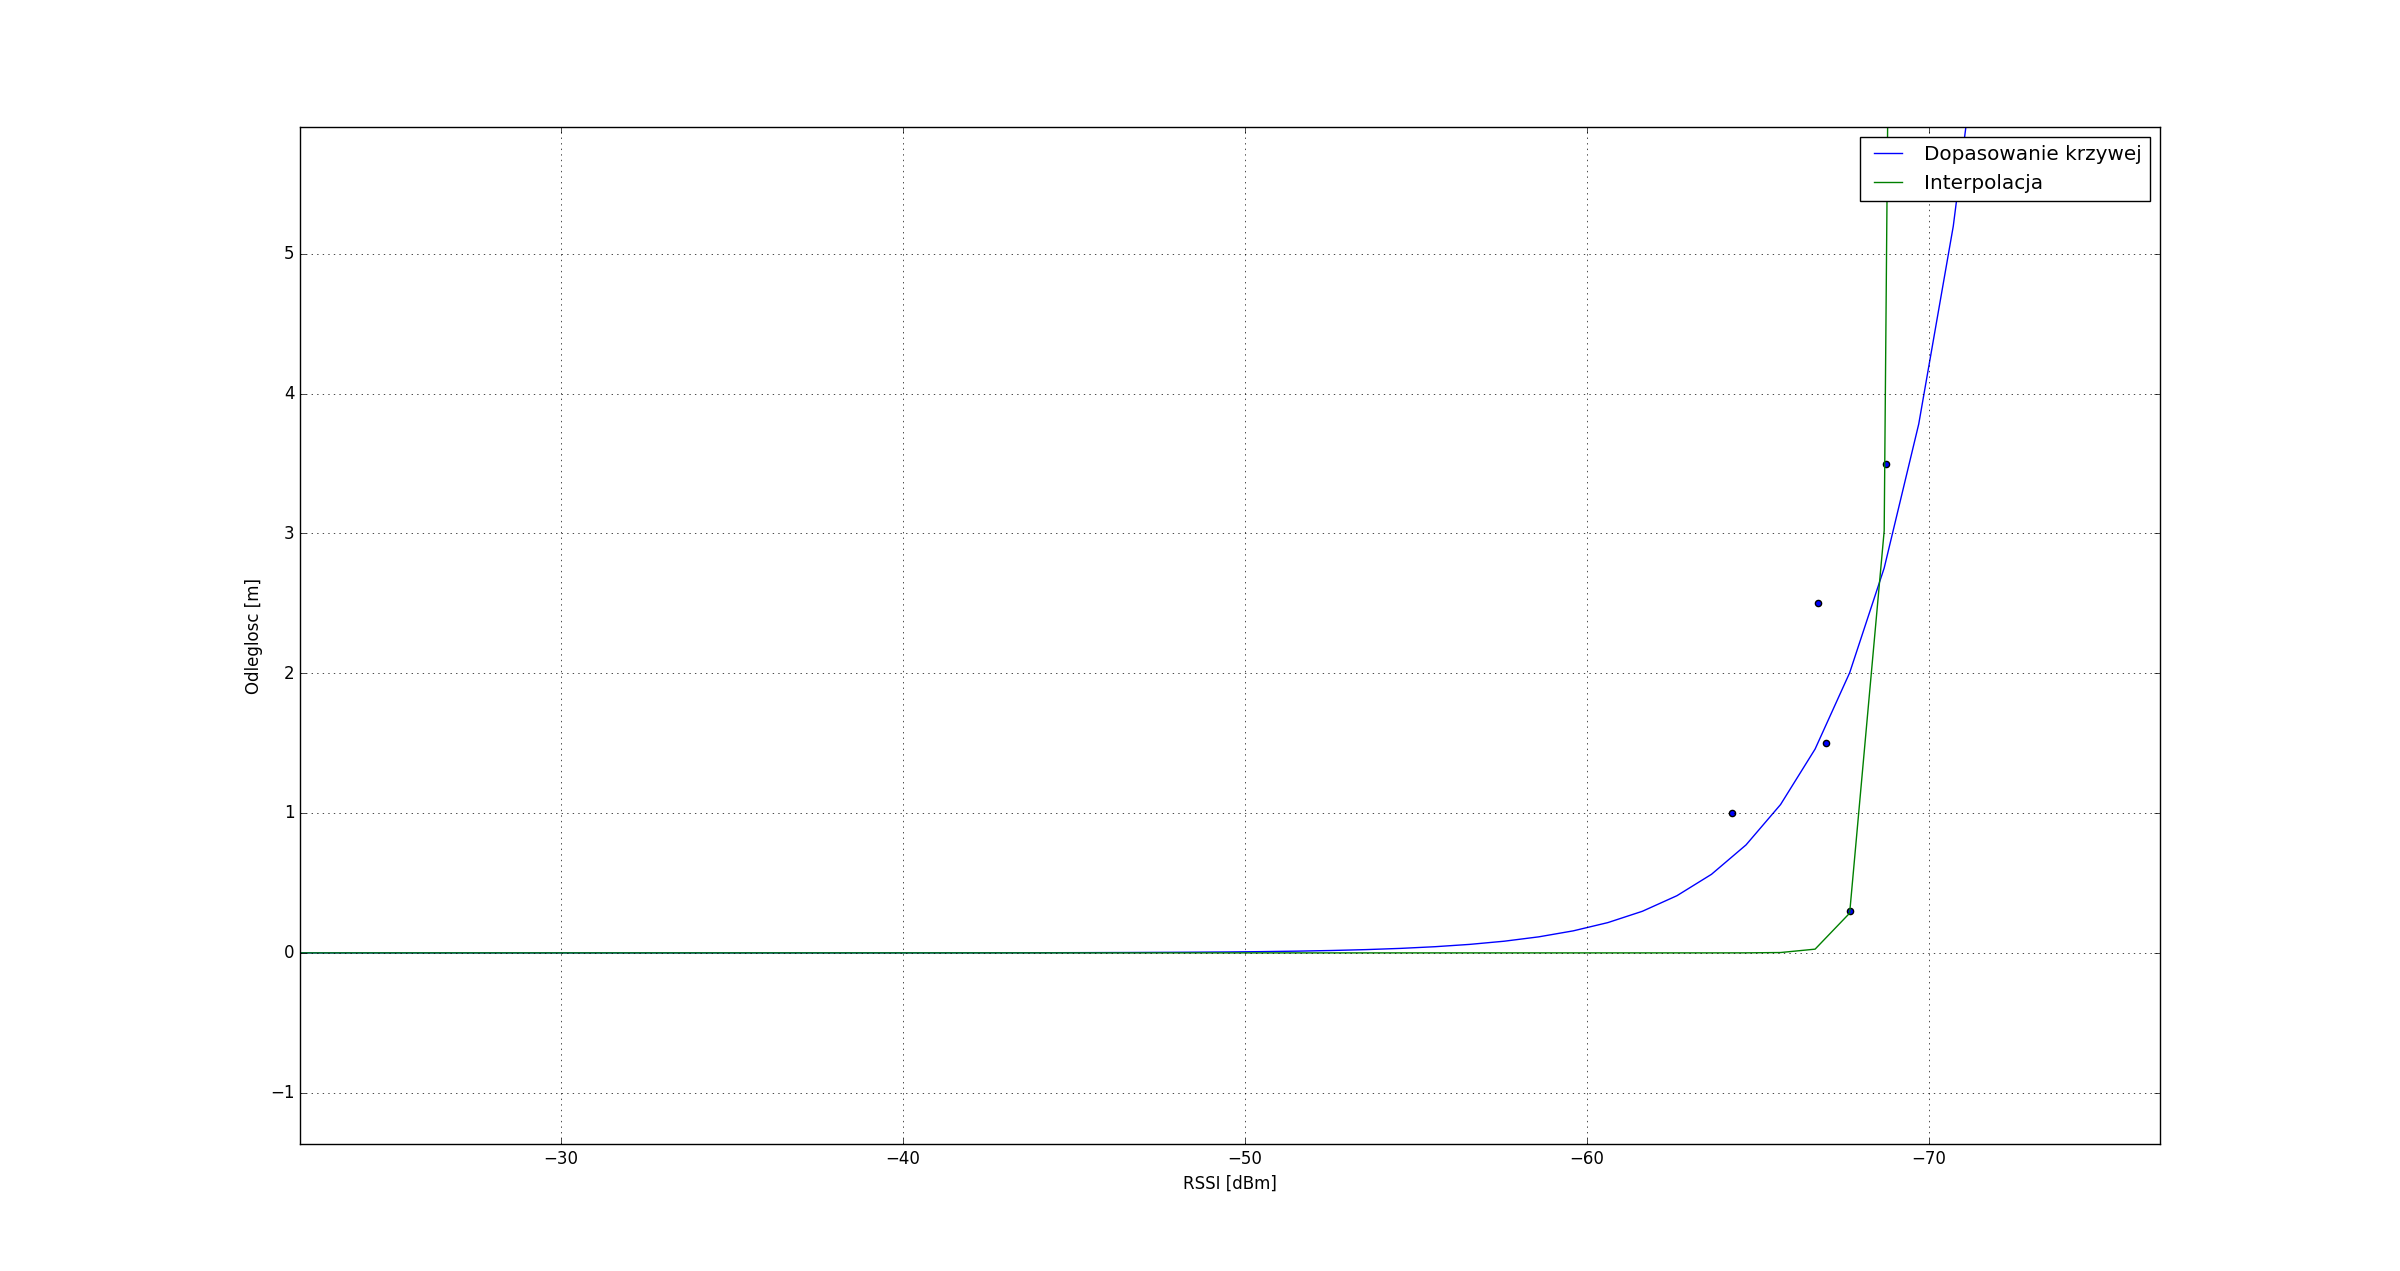
\includegraphics[width=1\textwidth]{img/strojenie-c.png}
\caption{Wyznaczanie modelu znacznika C}
\label{fig:strojenie-c}
\end{figure}

\subsubsection{Trilateracja}
Pierwsze próby lokalizacji za pomocą trilateracji przeprowadzono wykorzystując model wyznaczony w poprzednim punkcie metodą dopasowania krzywej. Jednakże, jak pokazuje rys. \ref{fig:trilat-przegryw}, nastawy te powodują bardzo duży rozrzut wyników pomiaru - większość wyznaczonych położeń robota wypada poza mapą i nie ma związku z rzeczywistym jego położeniem. Rys. \ref{fig:trilat-przegryw} obrazuje ten problem dla jednego punktu pomiarowego, jednakże podobnie duży rozrzut występuje również dla pozostałych punktów. Należy zwrócić uwagę na inną skalę osi wykresu \ref{fig:trilat-przegryw} w porównaniu do wykresów  \ref{fig:trilat-first} - \ref{fig:trilat-last}. Dyskusję możliwych przyczyn takiego zachowania przedstawiono w rozdziale \ref{ch:wnioski}.

Dlatego też podjęto próbę wyznaczenia właściwego modelu ręcznie, metodą prób i błędów. Bazując na modelach wyznacznonych automatycznie, wykorzystując narzędzie Rosbag oraz narzędzia do wykreślania zależności siły sygnału od odległości, dobrano model zapewniający wyniki o mniejszym rozrzucie:
\begin{equation}
 a=50, b=50
\end{equation}

Wyniki z wykorzystaniem modelu wyznaczonego ręcznie pokazują rys. \ref{fig:trilat-first} - \ref{fig:trilat-last}. Dla porównania, rysunki te, z wyjątkiem rys. \ref{fig:trilat-przegryw} posiadają jednakową skalę. Rysunek \ref{fig:trilat-przegryw} ma zmienioną skalę aby ukazać problem rozrzutu wyników. 

Na rysunkach, czerwony krzyżyk oznacza punkt odniesienia, niebieskie kropki symbolizują wyniki trilateracji. Na rysunku \ref{fig:referencyjne} przedstawiono położenie kolejnych punktów odniesienia.
\begin{figure}[H]
\centering
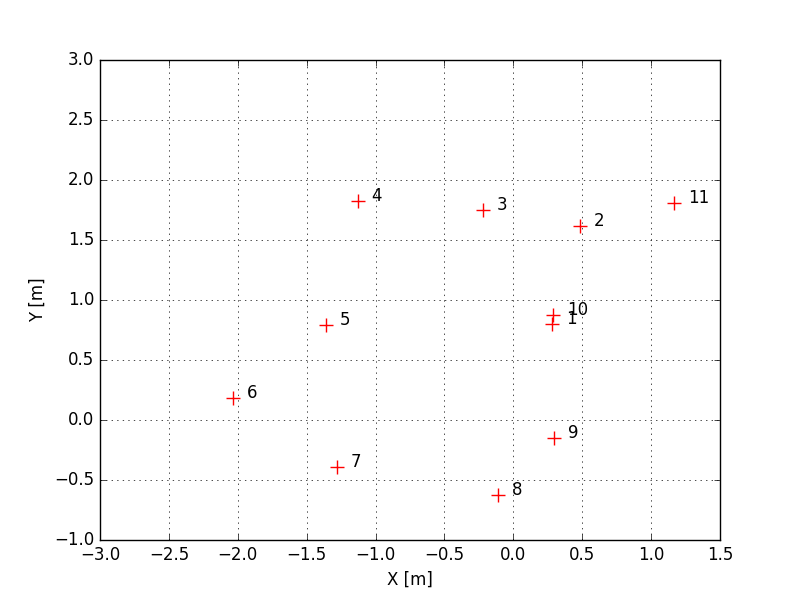
\includegraphics[width=0.7\textwidth]{img/references.png}
\caption{Położenie punktów pomiarowych.}
\label{fig:referencyjne}
\end{figure}
\begin{figure}[H]
\centering
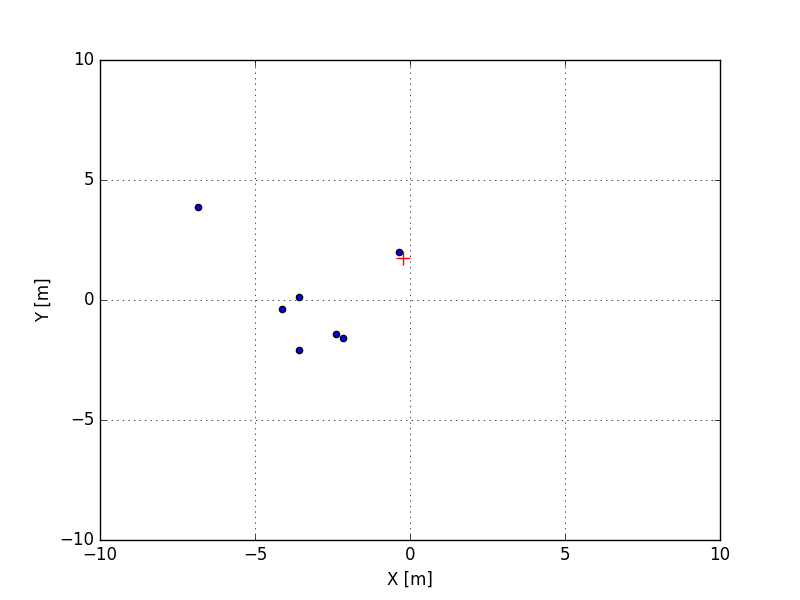
\includegraphics[width=0.7\textwidth]{img/trilat-przegryw.png}
\caption{Wyniki trilateracji dla modelu obliczonego przez dopasowanie krzywej}
\label{fig:trilat-przegryw}
\end{figure}
\begin{figure}[H]
\centering
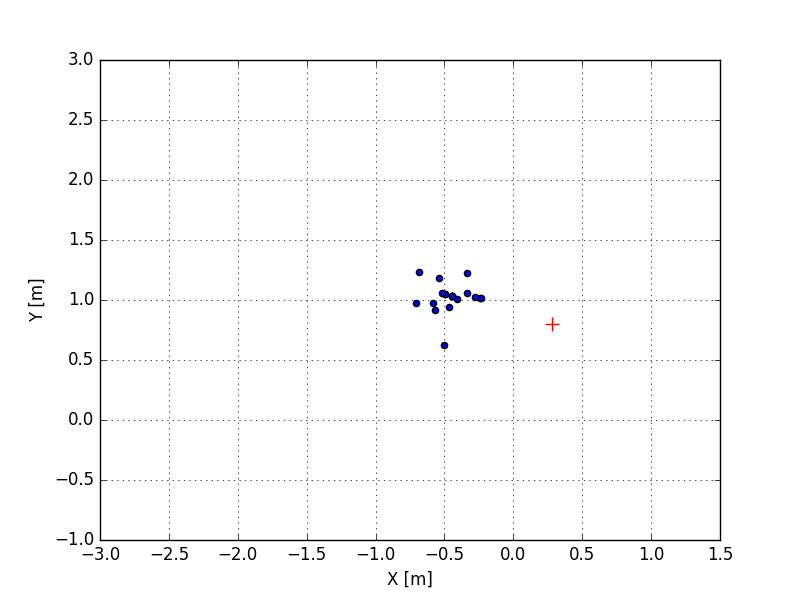
\includegraphics[width=0.7\textwidth]{img/trilat-map3-1.png}
\caption{Wyniki trilateracji dla ręcznie dobranego modelu - punkt 1}
\label{fig:trilat-first}
\end{figure}
\begin{figure}[H]
\centering
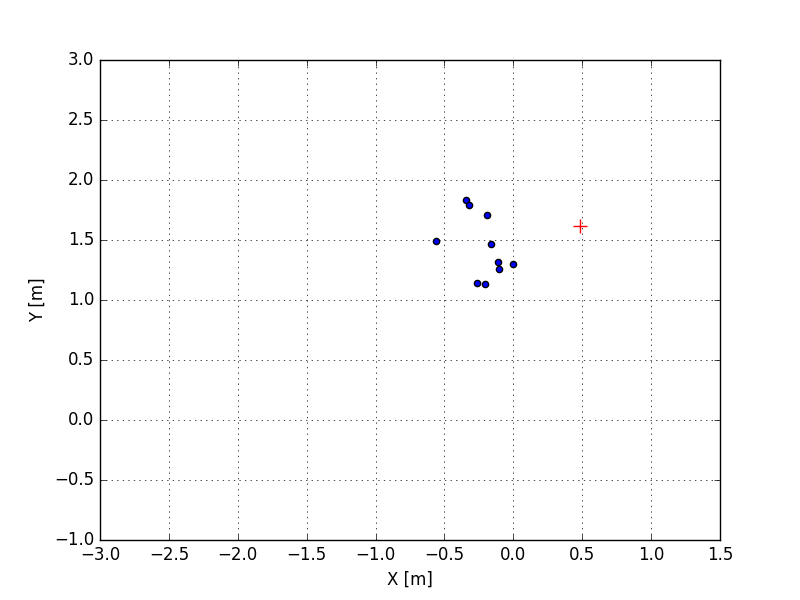
\includegraphics[width=0.7\textwidth]{img/trilat-map3-2.png}
\caption{Wyniki trilateracji dla ręcznie dobranego modelu - punkt 2}
\end{figure}
\begin{figure}[H]
\centering
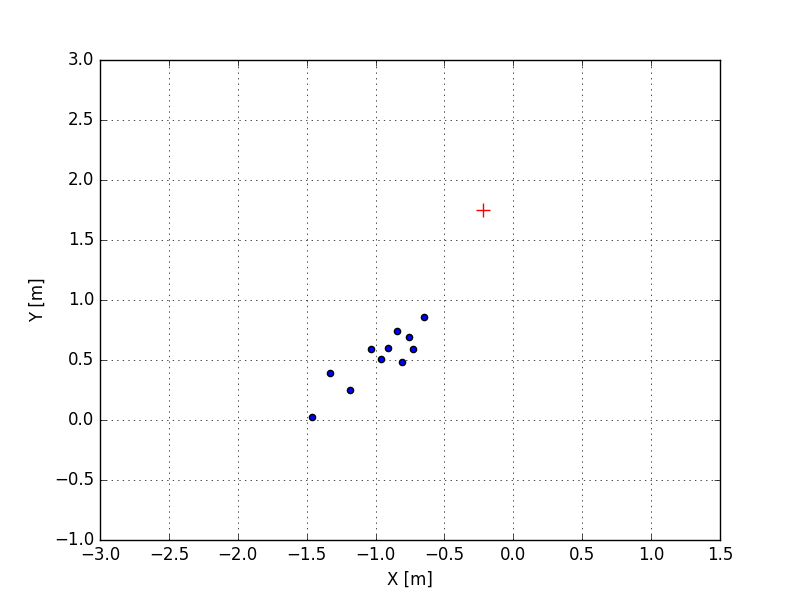
\includegraphics[width=0.7\textwidth]{img/trilat-map3-3.png}
\caption{Wyniki trilateracji dla ręcznie dobranego modelu - punkt 3}
\end{figure}
\begin{figure}[H]
\centering
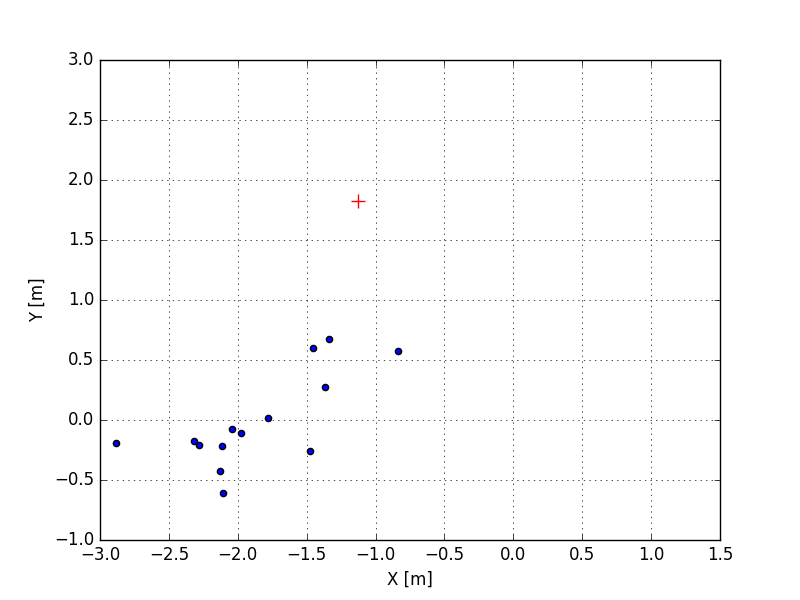
\includegraphics[width=0.7\textwidth]{img/trilat-map3-4.png}
\caption{Wyniki trilateracji dla ręcznie dobranego modelu - punkt 4}
\end{figure}
\begin{figure}[H]
\centering
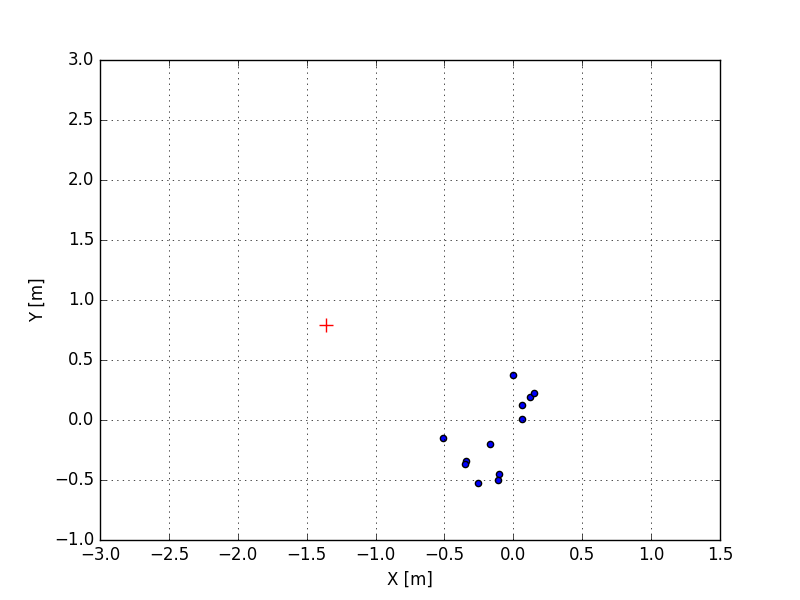
\includegraphics[width=0.7\textwidth]{img/trilat-map3-5.png}
\caption{Wyniki trilateracji dla ręcznie dobranego modelu - punkt 5}
\end{figure}
\begin{figure}[H]
\centering
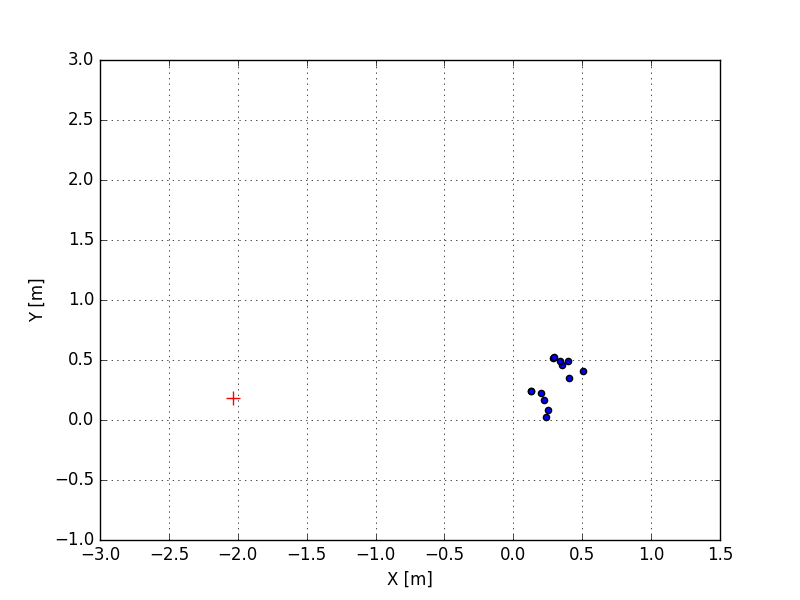
\includegraphics[width=0.7\textwidth]{img/trilat-map3-6.png}
\caption{Wyniki trilateracji dla ręcznie dobranego modelu - punkt 6}
\end{figure}
\begin{figure}[H]
\centering
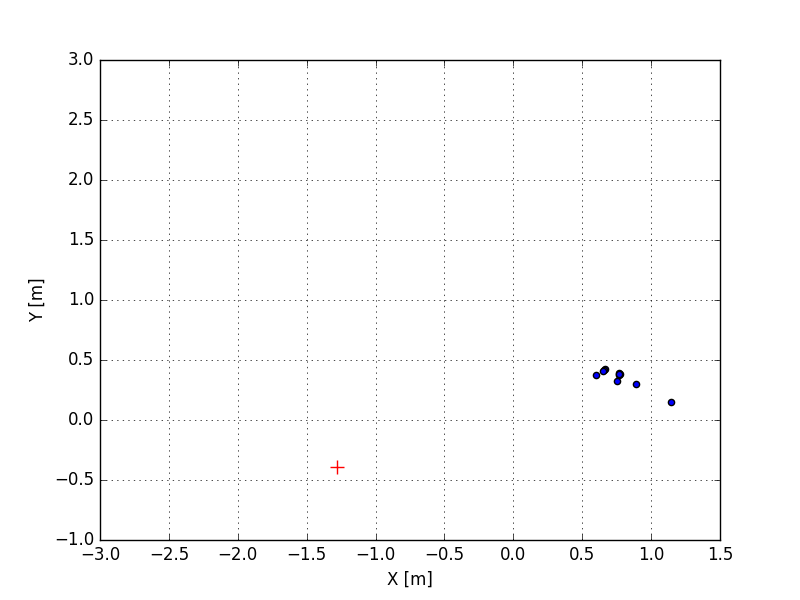
\includegraphics[width=0.7\textwidth]{img/trilat-map3-7.png}
\caption{Wyniki trilateracji dla ręcznie dobranego modelu - punkt 7}
\end{figure}
\begin{figure}[H]
\centering
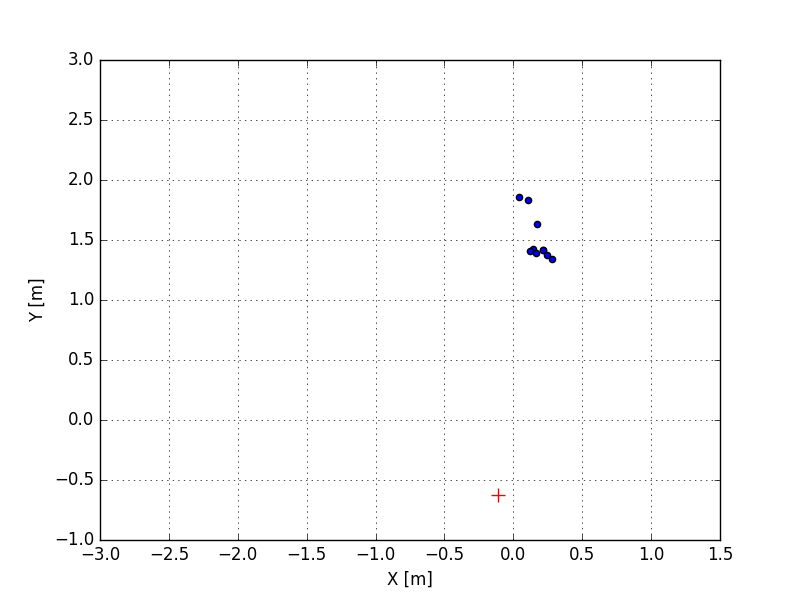
\includegraphics[width=0.7\textwidth]{img/trilat-map3-8.png}
\caption{Wyniki trilateracji dla ręcznie dobranego modelu - punkt 8}
\end{figure}
\begin{figure}[H]
\centering
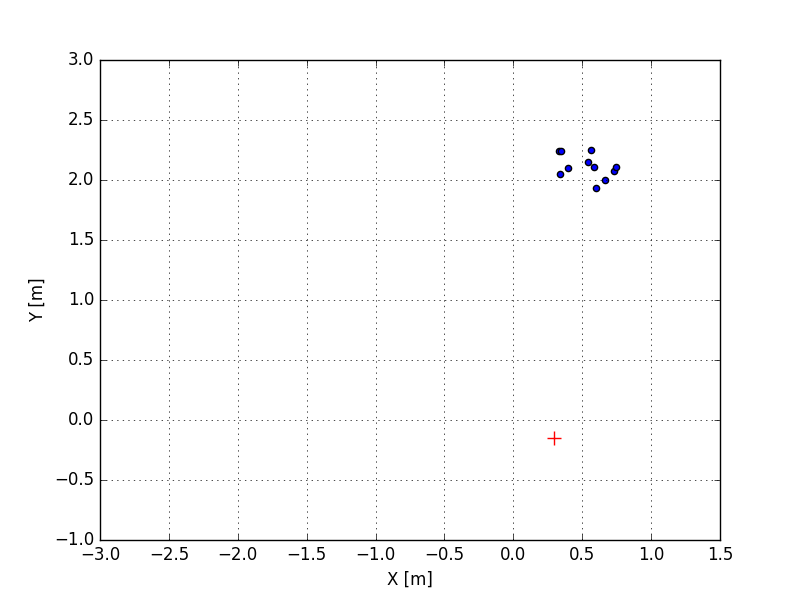
\includegraphics[width=0.7\textwidth]{img/trilat-map3-9.png}
\caption{Wyniki trilateracji dla ręcznie dobranego modelu - punkt 9}
\end{figure}
\begin{figure}[H]
\centering
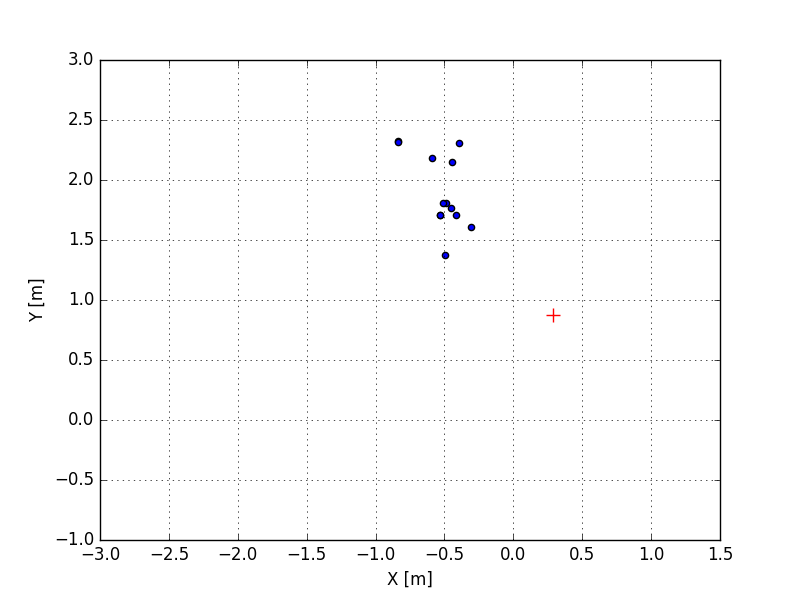
\includegraphics[width=0.7\textwidth]{img/trilat-map3-10.png}
\caption{Wyniki trilateracji dla ręcznie dobranego modelu - punkt 10}
\end{figure}
\begin{figure}[H]
\centering
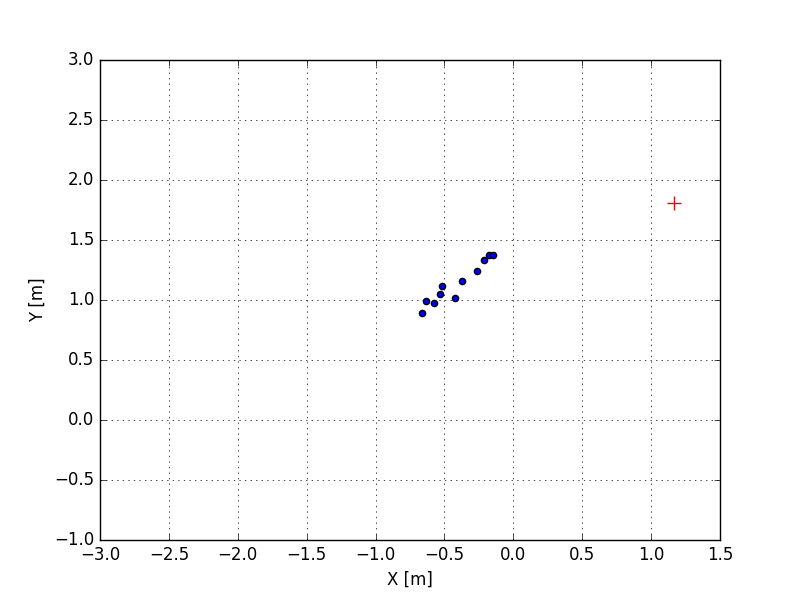
\includegraphics[width=0.7\textwidth]{img/trilat-map3-11.png}
\caption{Wyniki trilateracji dla ręcznie dobranego modelu - punkt 11}
\label{fig:trilat-last}
\end{figure}


\subsubsection{Filtr cząsteczkowy}
Jak wspomniano wcześniej, badanie filtra cząsteczkowego przeprowadzono na tym samym zbiorze danych co badania metody trilateracji. Podobnie jak w wypadku trilateracji, wykorzystano model wyznacznony ręcznie. Wyniki lokalizacji w poszczególnych punktach ukazują wykresy \ref{fig:pf-first} - \ref{fig:pf-last}. Można zauważyć, że na wykresach zaznaczono miejszą ilość punktów wynikowych niż w wypadku trilateracji. Ta różnica wynika z faktu, że wynik trilateracji jest publikowany w stałym interwale (1 sekunda), natomiast filtr cząsteczkowy jest przeliczany tylko wtedy, kiedy odległość liniowa lub kątowa pokonana przez robota i zmierzona za pomocą odometrii przekroczy pewien próg. Jest to związane z optymalizacją wydajności programu. Dlatego też, kiedy robot jest nieruchomy, nowe punkty nie są publikowane - bowiem byłyby identyczne jak poprzednie.


\begin{figure}[H]
\centering
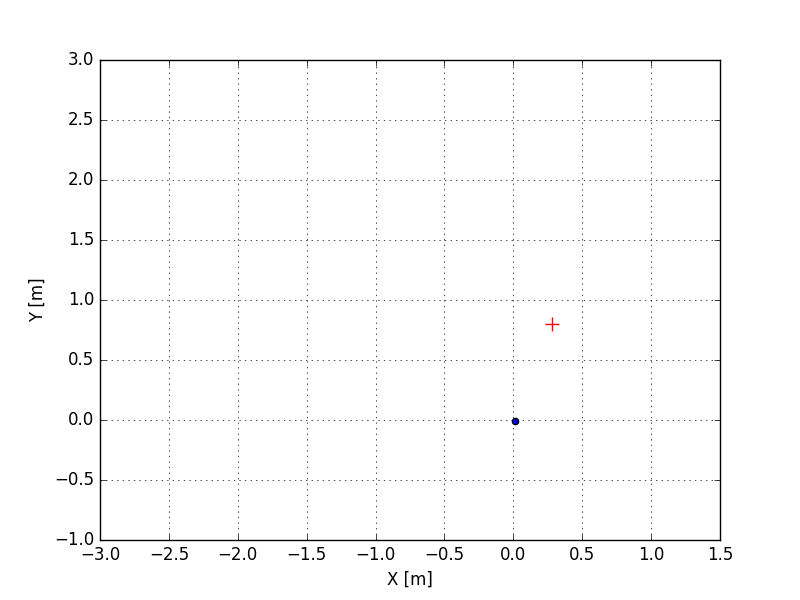
\includegraphics[width=0.7\textwidth]{img/pf-map3-1.png}
\caption{Wyniki lokalizacji za pomocą filtra cząsteczkowego dla ręcznie dobranego modelu - punkt 1}
\label{fig:pf-first}
\end{figure}
\begin{figure}[H]
\centering
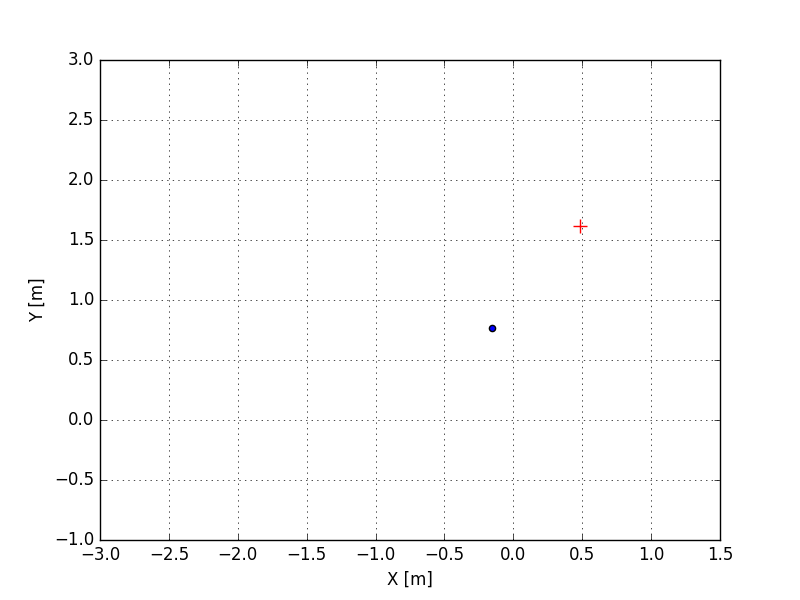
\includegraphics[width=0.7\textwidth]{img/pf-map3-2.png}
\caption{Wyniki lokalizacji za pomocą filtra cząsteczkowego dla ręcznie dobranego modelu - punkt 2}
\end{figure}
\begin{figure}[H]
\centering
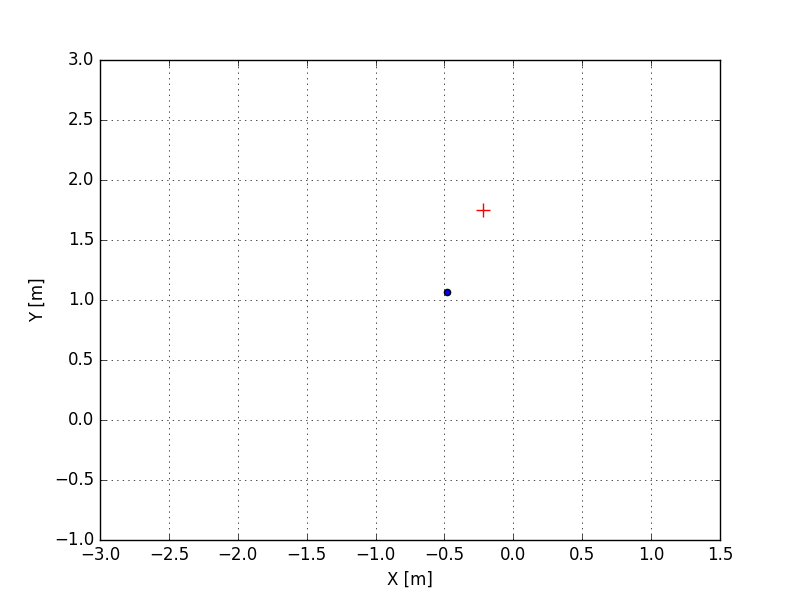
\includegraphics[width=0.7\textwidth]{img/pf-map3-3.png}
\caption{Wyniki lokalizacji za pomocą filtra cząsteczkowego dla ręcznie dobranego modelu - punkt 3}
\end{figure}
\begin{figure}[H]
\centering
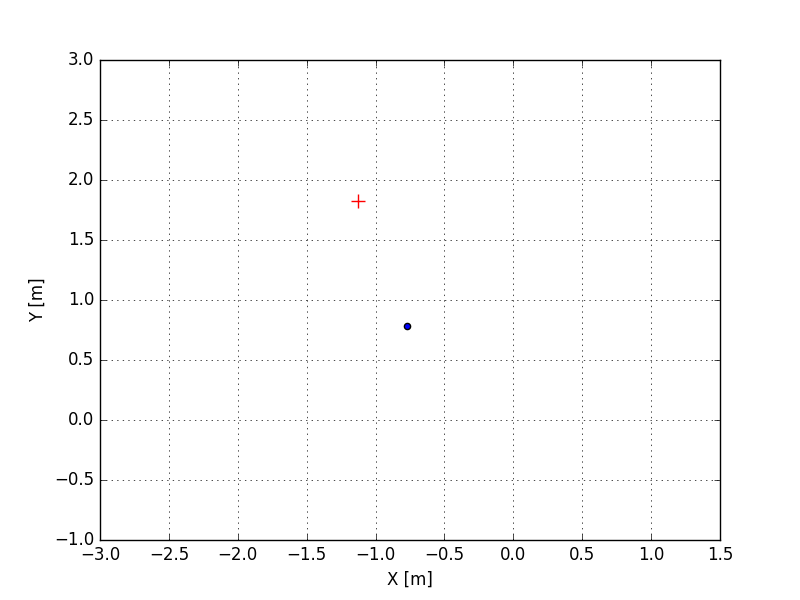
\includegraphics[width=0.7\textwidth]{img/pf-map3-4.png}
\caption{Wyniki lokalizacji za pomocą filtra cząsteczkowego dla ręcznie dobranego modelu - punkt 4}
\end{figure}
\begin{figure}[H]
\centering
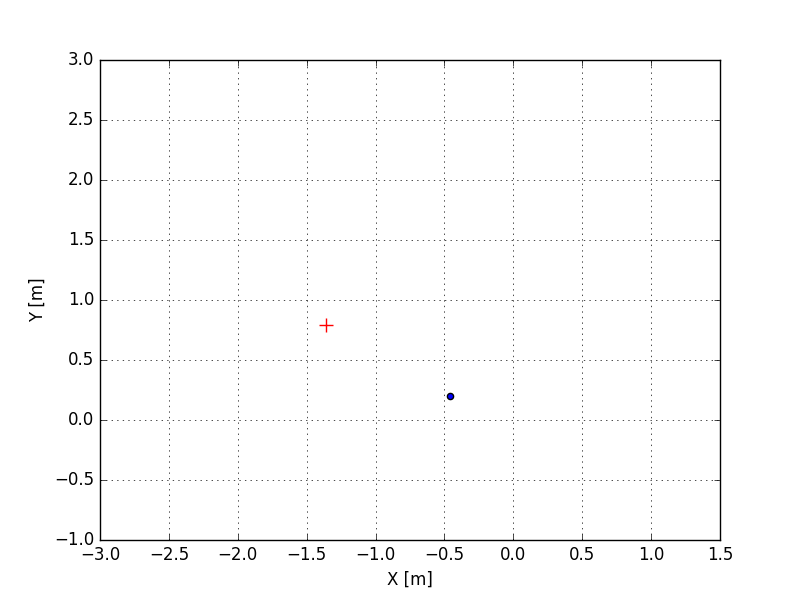
\includegraphics[width=0.7\textwidth]{img/pf-map3-5.png}
\caption{Wyniki lokalizacji za pomocą filtra cząsteczkowego dla ręcznie dobranego modelu - punkt 5}
\end{figure}
\begin{figure}[H]
\centering
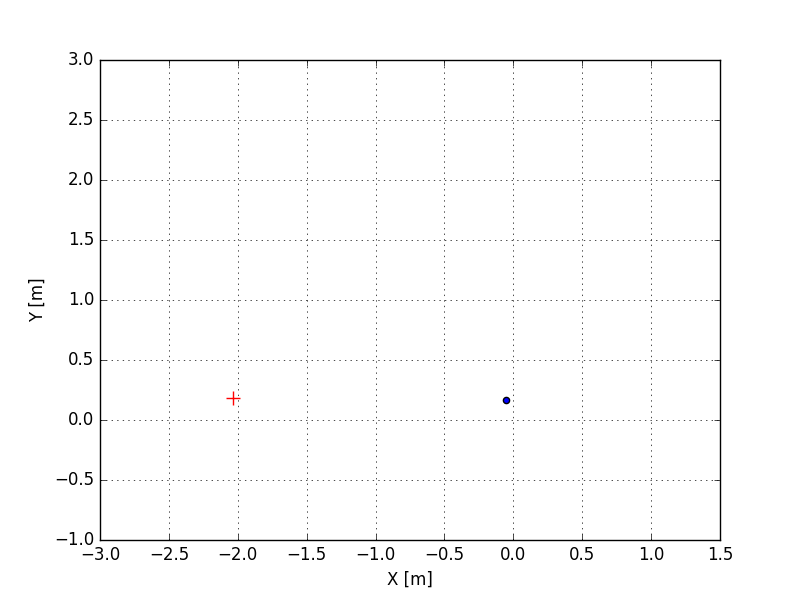
\includegraphics[width=0.7\textwidth]{img/pf-map3-6.png}
\caption{Wyniki lokalizacji za pomocą filtra cząsteczkowego dla ręcznie dobranego modelu - punkt 6}
\end{figure}
\begin{figure}[H]
\centering
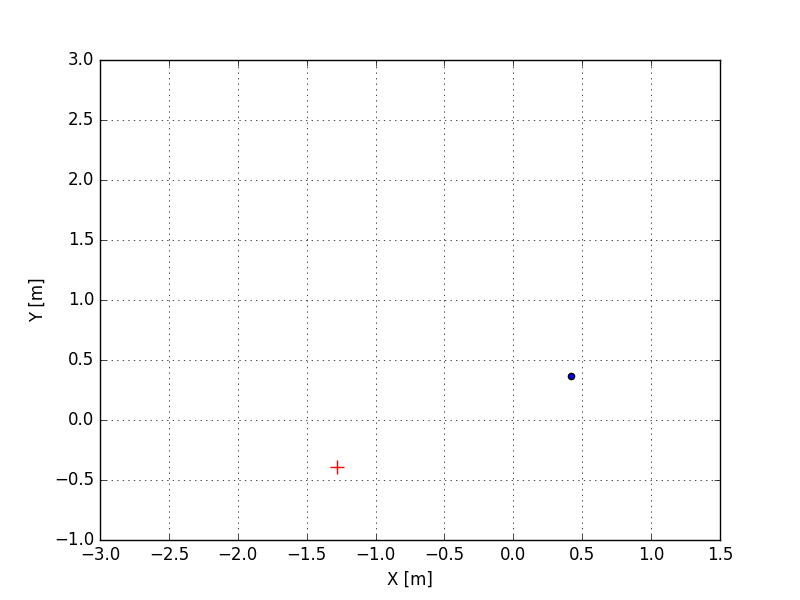
\includegraphics[width=0.7\textwidth]{img/pf-map3-7.png}
\caption{Wyniki lokalizacji za pomocą filtra cząsteczkowego dla ręcznie dobranego modelu - punkt 7}
\end{figure}
\begin{figure}[H]
\centering
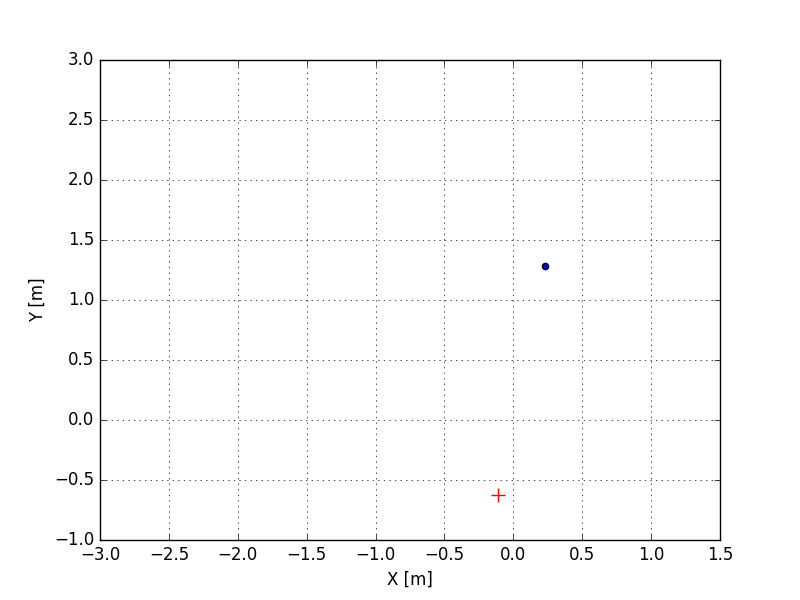
\includegraphics[width=0.7\textwidth]{img/pf-map3-8.png}
\caption{Wyniki lokalizacji za pomocą filtra cząsteczkowego dla ręcznie dobranego modelu - punkt 8}
\end{figure}
\begin{figure}[H]
\centering
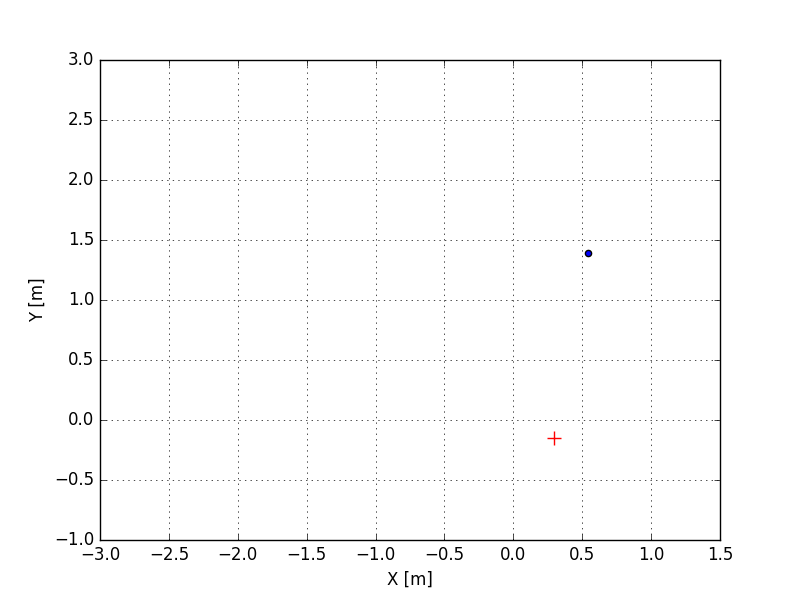
\includegraphics[width=0.7\textwidth]{img/pf-map3-9.png}
\caption{Wyniki lokalizacji za pomocą filtra cząsteczkowego dla ręcznie dobranego modelu - punkt 9}
\end{figure}
\begin{figure}[H]
\centering
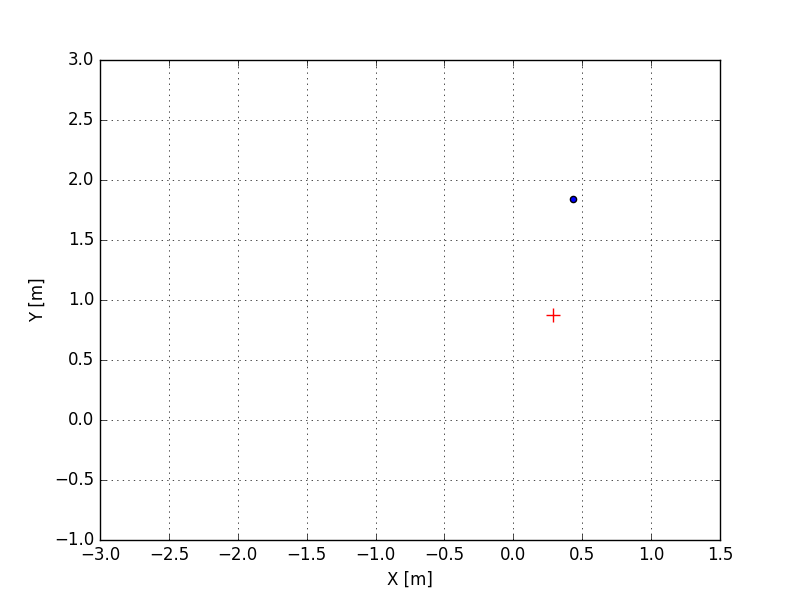
\includegraphics[width=0.7\textwidth]{img/pf-map3-10.png}
\caption{Wyniki lokalizacji za pomocą filtra cząsteczkowego dla ręcznie dobranego modelu - punkt 10}
\end{figure}
\begin{figure}[H]
\centering
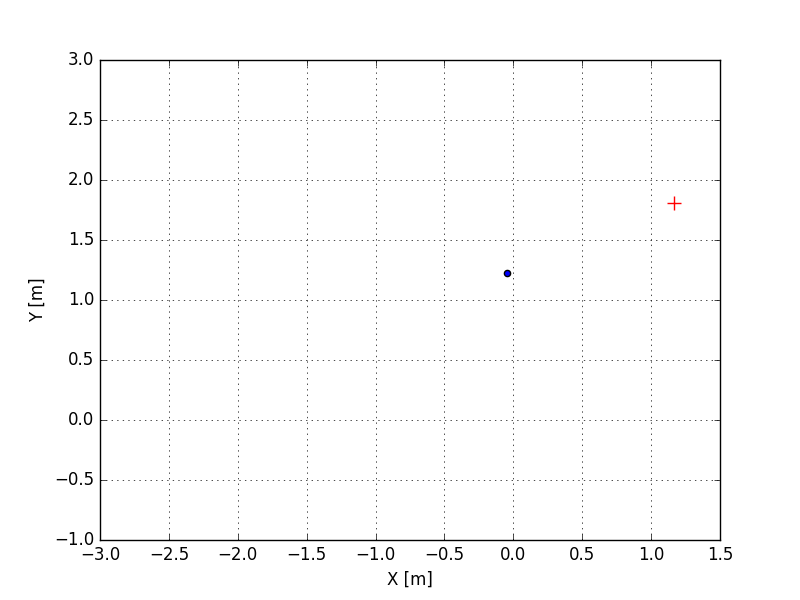
\includegraphics[width=0.7\textwidth]{img/pf-map3-11.png}
\caption{Wyniki lokalizacji za pomocą filtra cząsteczkowego dla ręcznie dobranego modelu - punkt 11}
\label{fig:pf-last}
\end{figure}

\section{Rozwiązanie problemu porwanego robota za pomocą lokalizacji BLE i AMCL}



% \chapter{Podsumowanie} % (fold)
\label{cha:podsumowanie}

Praca miała na celu projekt systemu do monitorowania zużycia mediów komunalnych.
Projektowany system miał pozwalać na wizualizację bieżących i historycznych stanów oraz powiadamiać o zdarzeniach niepożądanych takich jak braki odpowiedzi urządzeń sieciowych, co może świadczyć o ich awarii, lub o znaczących różnicach w stosunku do przewidywanego dobowego zużycia medium.

W trakcie pracy powstało oprogramowanie UMonit wspierające liczniki komunikujące się za pomocą protokołu M-Bus lub pozwalające, za pomocą innych narzędzi, na integrację z tym protokołem.
Projekt UMonit składał się z dwóch podprojektów UMonitApp oraz UMonitWeb.
UMonitApp zajmuje się odczytywanie liczników zgodnie z normą PN-EN 13757, zapisem danych pomiarowych oraz wykrywaniem błędów.
UMonitWeb jest narzędziem do przeglądania zebranych przez UMonitApp danych w formie listy ostatnich znanych wartości parametrów danego licznika lub wykresów zmiany tych parametrów.
Pozwala również na wylistowanie zdarzeń, które pojawiły się w systemie.

System ten może być z powodzeniem stosowany do celów rozliczeniowych, gdzie sześciominutowy interwał odczytów jest dopuszczalny.
Jest on łatwo integrowalny z infrastrukturą domową, gdzie używane są liczniki posiadające wyjścia impulsowe lub moduły komunikacyjne M-Bus.
Podłączenie do domowego routera pozwala na dostęp do danych z dowolnego komputera, laptopa, telefonu czy tabletu będących w sieci LAN tworzonej przez ten router.
Obsługa 250 urządzeń pozwala na zastosowanie rozwiązania w blokach mieszkalnych do monitorowania poszczególnych pięter lub całych budynków.

Ze względu dużą wartość interwału odczytów UMonit nie nadaje się do zastosowań przemysłowych, gdzie częstotliwości sprawdzania stanu parametrów powinna być wielokrotnie większa.

Błędy mogą pojawić się zarówno na etapie implementacji, jak i na etapie modelowania czy tworzenia założeń systemu.
Pierwsze mogą być trudne do wykrycia, a drugie kosztowne w rozwiązaniu.
Podczas implementacji pojawiło się wiele nieprzewidzianych problemów, które należało rozwiązać, aby móc kontynuować prace nad projektem.

Jednym z nich było rozgłaszanie komend \textit{echo} oraz \textit{status} w wielu interfejsach sieciowych.
Problem pojawił się, kiedy Odroid C1+ był połączony z konwerterem ETH2 za pomocą kabla ethernetowego oraz z lokalną siecią WiFi za pomocą zewnętrznej karty sieciowej.
Okazało się, że system Ubuntu 16.04 nie propagował rozgłoszeń typu $ 255.255.255.255 $ na wiele interfejsów, ponieważ urządzenie posiadało więcej niż jeden adres IP.
Rozwiązaniem było pobranie listy dostępnych interfejsów sieciowych i wysłanie komendy \textit{echo} lub \textit{status} na adres rozgłoszeniowy tego interfejsu.
Pomocna w uzyskaniu tych parametrów okazała się biblioteka Qt udostępniająca odpowiednie do tego klasy.

Kolejnym problemem było niespodziewane odrzucanie kilku kolejnych ramek.
Działo się to raz na kilkanaście odczytów.
Problem miał dwa źródła.
Pierwszym było założenie, że odbieranie i wstępne przetwarzanie danych może odbywać się niezależnie od procesu wysyłania danych.
Oznaczało to tyle, że bufory na dane nie były przygotowywane na odbiór nowych ramek.
Należało je wyczyścić przy każdym żądaniu.
Drugim źródłem była źle ustawiona wartość timeoutu, która powodowała zbyt wczesną ponowną próbę odczytania danych, co prowadziło do przerywania przez licznik poprzedniej transmisji.

UMonit nie jest jeszcze gotowym produktem mogącym być zainstalowanym w domu.
Wymaga jeszcze wiele testów kompatybilności z licznikami innych mediów oraz urządzeniami innych producentów.
W przyszłości system może być rozszerzony lub połączony z istniejącym systemem rachunkowym obliczającym wielkości opłat za zużywane media.
Notyfikacje mogłyby otrzymać różne priorytety określane automatycznie lub definiowane przez użytkownika.
UMonit może również pozwalać w przyszłości na definiowanie nowych alarmów przez użytkownika, który definiowałby także sposób powiadamiania o ich zajściu np. za pomocą maila lub SMS-a dla najbardziej krytycznych.

Do systemu mogłoby zostać dodane wsparcie dla protokołu zdalnego odczytu WM-Bus pozwalającego na zbieranie danych bez ingerencji w strukturę mieszkania w celu przeciągnięcia przewodów komunikacyjnych dla magistrali M-Bus.
Dodatkowo wprowadzić można system uwierzytelniania użytkowników w celu zabezpieczenia i ograniczenia dostępu do danych osobom niepowołanym.

Cel pracy został osiągnięty, a z założenia tworzonego systemu w pełni zrealizowane.
% chapter wnioski (end)

\listoffigures

\listoftables

\printbibliography

% \input{zalaczniki}
\end{document}
